% ============================================================
%  MASTER'S THESIS — MODULAR VERSION
%  Learning Motor Control Strategies in Musculoskeletal Systems
%  Using Deep Reinforcement Learning
%
%  Compile with: pdflatex -> biber -> pdflatex -> pdflatex
%  Or:           latexmk -pdf main.tex
%
%  File structure:
%    main.tex         ← this file (preamble + document skeleton)
%    Abstract.tex     ← standalone research abstract (compile separately)
%    frontmatter.tex  ← title page, dedication, acks, abstracts, TOC
%    chapter1.tex     ← General Introduction
%    chapter2.tex     ← State of the Art
%    chapter3.tex     ← Modelling and Simulation Environment
%    chapter4.tex     ← Theoretical Framework of DRL
%    chapter5.tex     ← Implementation and Experimental Methodology
%    chapter6.tex     ← Experimental Results and Analysis
%    chapter7.tex     ← Discussion
%    conclusion.tex   ← General Conclusion and Future Directions
%    appendices.tex   ← Appendices A–E
%    references.bib   ← BibTeX bibliography
% ============================================================

\documentclass[12pt, a4paper, oneside, openany]{report}

% ── Encoding & language ────────────────────────────────────
\usepackage[utf8]{inputenc}
\usepackage[T1]{fontenc}
\usepackage[english]{babel}

% ── Fonts ──────────────────────────────────────────────────
\usepackage{lmodern}
\usepackage{csquotes}

% ── Page layout ────────────────────────────────────────────
\usepackage[
  a4paper,
  top=25mm, bottom=25mm,
  left=30mm, right=25mm,
  headheight=15pt,
  headsep=10mm,
  footskip=12mm
]{geometry}

% ── Headers / Footers ──────────────────────────────────────
\usepackage{fancyhdr}
\pagestyle{fancy}
\fancyhf{}
\renewcommand{\headrulewidth}{0.4pt}
\renewcommand{\footrulewidth}{0.4pt}
\fancyhead[L]{\small\slshape Musculoskeletal Model \& RL}
\fancyhead[R]{\small\slshape\leftmark}
\fancyfoot[R]{\small\thepage}
\fancypagestyle{plain}{%
  \fancyhf{}
  \renewcommand{\headrulewidth}{0pt}
  \fancyfoot[R]{\small\thepage}
}

% ── Maths ──────────────────────────────────────────────────
\usepackage{amsmath, amssymb, amsthm, mathtools}
\usepackage{bm}
\usepackage{siunitx}
\sisetup{output-decimal-marker={,}, group-separator={\,}, detect-all}

% ── Graphics & colors ──────────────────────────────────────
\usepackage[dvipsnames, table]{xcolor}
\usepackage{graphicx}
\usepackage{tikz}
\usetikzlibrary{arrows.meta, positioning, shapes, decorations.pathmorphing,
                calc, shadows.blur, patterns}
\usepackage{pgfplots}
\pgfplotsset{compat=1.18}
\usepackage{pgf-pie}

% ── Define colour palette ──────────────────────────────────
\definecolor{navyblue}{HTML}{1F3864}
\definecolor{accentblue}{HTML}{2E5FA3}
\definecolor{lightblue}{HTML}{D9E8F5}
\definecolor{midgrey}{HTML}{555555}
\definecolor{codebg}{HTML}{F5F5F5}
\definecolor{coderule}{HTML}{2E5FA3}
\definecolor{successgreen}{HTML}{1B7340}
\definecolor{warningorange}{HTML}{C75000}
\definecolor{deepred}{HTML}{A81E2B}

% ── Tables ─────────────────────────────────────────────────
\usepackage{booktabs}
\usepackage{longtable}
\usepackage{array}
\usepackage{multirow}
\usepackage{tabularx}
\usepackage{colortbl}
\newcolumntype{L}[1]{>{\raggedright\arraybackslash}p{#1}}
\newcolumntype{C}[1]{>{\centering\arraybackslash}p{#1}}
\newcolumntype{R}[1]{>{\raggedleft\arraybackslash}p{#1}}

% ── Code listings ──────────────────────────────────────────
\usepackage{listings}
\lstset{
  backgroundcolor = \color{codebg},
  basicstyle      = \ttfamily\footnotesize,
  breaklines      = true,
  captionpos      = b,
  commentstyle    = \color{black}\itshape,
  frame           = leftline,
  framerule       = 2pt,
  rulecolor       = \color{accentblue},
  keywordstyle    = \color{black}\bfseries,
  stringstyle     = \color{black},
  numbers         = left,
  numberstyle     = \tiny\color{black},
  numbersep       = 8pt,
  showstringspaces= false,
  tabsize         = 4,
  xleftmargin     = 14pt,
}
\lstdefinelanguage{Python3}{
  language     = Python,
  morekeywords = {True, False, None, self, def, class, import, from,
                  return, yield, with, as, async, await, lambda},
}
\lstdefinelanguage{XML}{
  morestring   = [s]{"}{"},
  morestring   = [s]{'}{'},
  morecomment  = [s]{<!--}{-->},
  morekeywords = {mujoco, worldbody, body, joint, geom, site, tendon,
                  spatial, actuator, muscle, sensor, jointpos, option,
                  compiler},
  sensitive    = false,
}

% ── Hyperlinks & PDF meta ──────────────────────────────────
\usepackage[
  colorlinks = true,
  linkcolor  = black,
  citecolor  = black,
  urlcolor   = black,
]{hyperref}
\usepackage[nameinlink, noabbrev]{cleveref}

% ── Bibliography ───────────────────────────────────────────
\usepackage[
  backend    = biber,
  style      = numeric,
  sorting    = none,
  maxcitenames = 2,
  maxbibnames = 6,
]{biblatex}
\addbibresource{references.bib}

% ── Misc utilities ─────────────────────────────────────────
\usepackage{caption}
\captionsetup{labelfont=bf, font=small, labelsep=period}
\usepackage{subcaption}
\usepackage{float}
\usepackage{enumitem}
\usepackage{setspace}
\usepackage{emptypage}
\usepackage{tocloft}
\usepackage[nottoc]{tocbibind}
\usepackage{chngcntr}
\usepackage{xspace}
\counterwithin{figure}{chapter}
\counterwithin{table}{chapter}
\counterwithin{equation}{chapter}
\usepackage{epigraph}
\setlength{\epigraphwidth}{0.75\textwidth}
\raggedbottom
\emergencystretch=2em
\hfuzz=20pt
\hbadness=10000
\vbadness=10000

% ── Chapter styling ────────────────────────────────────────
\usepackage{titlesec}
\titleformat{\chapter}[block]
  {\normalfont\huge\bfseries\color{black}}
  {\thechapter}
  {0.75em}
  {}

\titleformat{name=\chapter,numberless}[block]
  {\normalfont\huge\bfseries\color{black}}
  {}
  {0pt}
  {}

\titlespacing*{\chapter}{0pt}{0pt}{24pt}

\titleformat{\section}
  {\normalfont\large\bfseries\color{black}}
  {\thesection}{1em}{}

\titleformat{\subsection}
  {\normalfont\normalsize\bfseries\color{black}}
  {\thesubsection}{1em}{}

\titleformat{\subsubsection}
  {\normalfont\normalsize\itshape\color{black}}
  {\thesubsubsection}{1em}{}

% ── Custom commands ────────────────────────────────────────
\newcommand{\RL}{RL}
\newcommand{\DR}{\textsc{DR}\xspace}
\newcommand{\DRL}{DRL}
\newcommand{\MuJoCo}{MuJoCo}
\newcommand{\opensource}{open-source\xspace}
\newcommand{\DDPG}{\textsc{DDPG}\xspace}
\newcommand{\TD}{\textsc{TD3}\xspace}
\newcommand{\TDIII}{\textsc{TD3}\xspace}
\newcommand{\PPO}{\textsc{PPO}\xspace}
\newcommand{\SAC}{\textsc{SAC}\xspace}
\newcommand{\eg}{\textit{e.g.}\xspace}
\newcommand{\ie}{\textit{i.e.}\xspace}
\newcommand{\norm}[1]{\left\lVert #1 \right\rVert}
\newcommand{\E}{\mathbb{E}}
\newcommand{\R}{\mathbb{R}}
\newcommand{\lnorm}{\tilde{l}}
\newcommand{\vnorm}{\tilde{v}}

\newcommand{\frontmatter}{%
  \clearpage
  \hypersetup{pageanchor=false}%
  \pagenumbering{roman}%
  \setcounter{page}{1}%
  \pagestyle{plain}%
}
\newcommand{\mainmatter}{%
  \clearpage
  \hypersetup{pageanchor=true}%
  \pagenumbering{arabic}%
  \setcounter{page}{1}%
  \pagestyle{fancy}%
}
\newcommand{\backmatter}{\clearpage}
\let\cleardoublepage\clearpage
\newcommand{\frontchapter}[1]{%
  \clearpage
  \chapter*{#1}%
  \markboth{#1}{#1}%
  \phantomsection
  \addcontentsline{toc}{chapter}{#1}%
}

% ── Theorem-like environments ──────────────────────────────
\newtheorem{definition}{Definition}[chapter]
\newtheorem{proposition}{Proposition}[chapter]
\newtheorem{remarque}{Remark}[chapter]

% ── Line spacing ───────────────────────────────────────────
\setstretch{1.3}

% ===========================================================
\begin{document}
% ===========================================================

\hypersetup{
  pdftitle   = {Master's Thesis - Musculoskeletal Model and RL},
  pdfauthor  = {Mohamed Naceur Hammami},
  pdfsubject = {Computational biomechanics and Deep Reinforcement Learning}
}

% ── Front matter (roman page numbers) ─────────────────────
\frontmatter
% frontmatter.tex contains: title page, dedication, acknowledgements,
% executive summary (French), abstract (English), abbreviations,
% symbols, table of contents, list of figures, list of tables.
% ===========================================================
%  TITLE PAGE
% ===========================================================
\begin{titlepage}
\begin{center}

{\small\textsc{Republic of Tunisia}\\
Ministry of Higher Education and Scientific Research}

\vspace{0.3cm}
\rule{\textwidth}{1.5pt}
\vspace{0.2cm}

{\large\bfseries\color{black}
University of Carthage --- École Polytechnique de Tunisie \\[4pt]}

\vspace{1.2cm}

{\Large\bfseries\color{black} MASTER'S THESIS}\\[0.3cm]
{\normalsize Submitted in partial fulfillment of the requirements for the degree of}\\[0.3cm]
{\large\bfseries\color{black}
MASTER'S IN COMPLEX AND INTELLIGENT SYSTEMS}

\vspace{1.2cm}
\rule{\textwidth}{0.8pt}
\vspace{0.5cm}

{\LARGE\bfseries\color{black}
Learning Motor Control Strategies \\[6pt]
in Musculoskeletal Systems Using \\[6pt]
Reinforcement Learning\\[6pt]
}

\vspace{0.5cm}
\rule{\textwidth}{0.8pt}

\vspace{1.5cm}
\begin{minipage}[t]{0.48\textwidth}
\raggedright
\textbf{Presented by:}\\[6pt]
{\large M.~\textit{Mohamed Naceur Hammami}}
\end{minipage}
\hfill
\begin{minipage}[t]{0.48\textwidth}
\raggedleft
\textbf{Supervised by:}\\[6pt]
Prof.~\textit{Taysir Rezgui}
\end{minipage}

\vfill
\rule{\textwidth}{0.8pt}\\[0.3cm]
{\large\bfseries Academic Year 2025--2026}

\end{center}
\end{titlepage}

% ===========================================================
%  DEDICATION
% ===========================================================
\cleardoublepage
\thispagestyle{empty}
\vspace*{5cm}
\begin{flushright}
\itshape\large
To my parents, an inexhaustible source of love and support,\\[4pt]
whose sacrifices made this work possible.\\[8pt]
To my brother and sisters, faithful companions at every moment.\\[8pt]
To my friends and colleagues, for their constant kindness.\\[8pt]
To all those affected by neurological injury, who remind us\\
that scientific research must serve human dignity.\\[16pt]
\normalsize\bfseries\color{black} I humbly dedicate this modest work to you.
\end{flushright}

% ===========================================================
%  ACKNOWLEDGEMENTS
% ===========================================================
\frontchapter{Acknowledgements}

At the completion of this work, I would like to express my deep gratitude to all the
people who contributed, directly or indirectly, to its realisation.

First and foremost, I extend my most sincere thanks to my thesis supervisor,
Professor~Taysir Rezgui, whose availability, wise advice, and rigorous guidance were
invaluable throughout this project. Their expertise in computational biomechanics has been an intellectual model that I will strive to draw inspiration from for years to come.

I also wish to express my gratitude to the entire teaching staff of the Computer
Engineering and Cyber-Physical Systems Department at the École Polytechnique de Tunisie,
who provided me with the theoretical and methodological foundations necessary for the
successful completion of this program.

I warmly thank the members of the jury for the interest they have shown in this work
and for agreeing to evaluate it, thereby devoting a valuable part of their time to its
critical reading.

My thanks also go to the \textit{open-source} scientific community --- the developers of
\MuJoCo{}, Gymnasium, Stable-Baselines3, PyTorch, Optuna, and the Python libraries used
throughout this work --- whose efforts greatly facilitated my experiments, and without
whom reproducible reinforcement-learning research would be far more difficult.

Finally, I thank my family and loved ones for their unwavering moral support and their
patience throughout this academic journey.

\bigskip\noindent\hfill{\large\bfseries\color{black} To all of you, thank you.}

% ===========================================================
%  ABSTRACT — FRENCH (EXECUTIVE SUMMARY)
% ===========================================================
\frontchapter{Executive Summary}

Because nine muscles actuate four degrees of freedom, infinitely many force
distributions produce any given arm movement, and the movement itself can never
reveal which one the controller used. Biomechanics resolves this indeterminacy
with a minimum-effort criterion; this thesis asks whether a \textit{Deep
Reinforcement Learning} (\DRL{}) controller, trained only on a reaching reward,
arrives at the same per-muscle force distribution.

The work began from a different question --- whether a trained policy could
replace the iterative Newton--Raphson muscle solver cheaply at inference time ---
and that premise did not survive measurement. A directly solved classical
load-sharing problem runs in \SI{23.9}{\micro\second} against the network's
\SI{288.8}{\micro\second}, so no speed advantage is claimed anywhere in this
work.

A four-degree-of-freedom articulated multi-body dynamic model driven by nine
muscles was developed in \MuJoCo{} \parencite{Todorov2012}. The model specifies a
Hill-type muscle representation \parencite{Hill1938, Zajac1989}, including the contractile element with
its force-length~(FL) and force-velocity~(FV) relationships, the series elastic
element~(SEE) modelling the tendon, the parallel elastic element~(PEE), pennation-angle
dynamics, and neural activation dynamics~\parencite{Thelen2003}. Numerical integration of
the tendon-fibre equilibrium equation is handled with an iterative Newton--Raphson
method. The resulting system is wrapped as a Gymnasium simulation environment.

Four \DRL{} algorithms were implemented with Stable-Baselines3
\parencite{Raffin2021} and compared: DDPG \parencite{Lillicrap2016}, TD3
\parencite{Fujimoto2018}, SAC \parencite{Haarnoja2018}, and PPO
\parencite{Schulman2017}, alongside a random policy and a PD impedance
controller as baselines. Five configurations were trained for $10^5$ steps with
three seeds each; the best configuration was additionally trained to
$3{\times}10^5$ steps and evaluated over fifty episodes.

The central analysis compares the learned muscle forces against those prescribed
by classical static optimisation on the identical movements. The learned
controller reproduces the coordination pattern of the classical solution ---
correlation $0{,}81 \pm 0{,}04$ over five independent training runs; pattern
cosine $0{,}813$ against a shuffled null of $0{,}372$ --- while expending
$1{,}91 \pm 0{,}15$ times the minimum effort required to generate the same joint
torques, the excess concentrated in co-contraction of the elbow antagonists. A
properly tuned conventional controller solving the same load-sharing problem
explicitly attains $1{,}263$, so the learned policy uses about 51~\% more effort
than is achievable rather than 91~\% more than an unattainable ideal. Raising the
reward's effort weight closes most of that gap, to $1{,}304 \pm 0{,}025$ against
that floor.

Two secondary results follow. An error plateau at \SI{0.10}{\meter} survived
three reward redesigns and a fourfold correction to the training budget;
one-at-a-time ablation over five hyperparameters identifies the discount factor
as its sole cause, recovering $106$~\% of the default-to-tuned interval where the
other four recover nothing. Its default horizon of 100 steps spanned the whole
episode against a reach completing in 25. And configuration proved to dominate algorithm choice: with every algorithm
given a correctly matched discount factor, \SI{0.060}{\meter} separates the best
off-policy method from the second, while correcting the discount factor within a
single algorithm is worth \SI{0.165}{\meter} --- about three times as much.

The results rest on three seeds for the algorithm comparison and five for the
principal analysis. No significance testing is reported. The strict success
criterion --- one that a privileged controller satisfies only $7$~\% of the time
--- is met in $0$--$20$~\% of episodes depending on seed, a twentyfold spread
under identical settings that identifies it as noise. Limitations are set out in
full in the general conclusion.

\bigskip
\noindent\textbf{Keywords:} Musculoskeletal model, \MuJoCo{}, Hill model, Static
optimisation, Muscle redundancy, Deep Reinforcement Learning, Motor control,
PPO, SAC, TD3, DDPG, Co-contraction, Discount factor.

% ===========================================================
%  ABSTRACT — ENGLISH
% ===========================================================
\begin{otherlanguage}{english}
\frontchapter{Abstract}

Nine muscles actuate four degrees of freedom in the model studied here, so
infinitely many force distributions produce any given movement and the movement
cannot reveal which was used. Biomechanics resolves this indeterminacy by a
minimum-effort criterion. This thesis asks whether a \textit{Deep Reinforcement
Learning}~(\DRL{}) controller, trained only on a reaching reward, recovers the
same per-muscle force distribution, and under what conditions on the training
objective.

The work was begun on a different premise --- that a trained policy might replace
the iterative Newton--Raphson muscle solver cheaply at inference time. That
premise did not survive measurement: a directly solved classical load-sharing
problem takes \SI{23.9}{\micro\second} against the network's
\SI{288.8}{\micro\second}. The latency argument is withdrawn in full.

A four-degree-of-freedom multi-body articulated dynamic model driven by nine
muscles was developed using the \MuJoCo{} physics engine
\parencite{Todorov2012}. The model specifies a Hill-type muscle model \parencite{Hill1938, Zajac1989} comprising: a contractile
element~(CE) governed by force-length~(FL) and force-velocity~(FV) relationships; a
series elastic element~(SEE) representing the tendon; a parallel elastic element~(PEE);
pennation-angle dynamics; and first-order activation dynamics \parencite{Thelen2003}.
The tendon-fibre equilibrium equation is numerically resolved via Newton-Raphson
iteration at each simulation step.

Four \DRL{} algorithms were implemented and benchmarked: DDPG
\parencite{Lillicrap2016}, TD3 \parencite{Fujimoto2018}, SAC \parencite{Haarnoja2018},
and PPO \parencite{Schulman2017}, alongside two reference baselines: a random policy
and a PD impedance controller. Five configurations were trained for $10^5$ steps
with three seeds each, and the best configuration additionally to
$3{\times}10^5$ steps with fifty-episode evaluation.

The central contribution is a per-muscle load-sharing comparison between the
learned solution and classical static optimisation, posed on the identical
trajectory with the identical required joint torques and verified to machine
precision. It is a conditional comparison --- static optimisation never chooses a
trajectory of its own --- and therefore bears on force distribution, not on the
realism of the movement. The
controller reproduces the coordination structure of the classical solution
(Pearson $r = 0.81 \pm 0.04$ over five seeds; pattern cosine $0.813$ against a
shuffled null of $0.372$) at a fixed, branch-free inference cost, but expends
$1.91 \pm 0.15$ times the minimum effort needed for the same joint torques, the
excess concentrated in elbow antagonist co-contraction. Raising the reward's
effort weight reduces that ratio to $1.304 \pm 0.025$ against the $1.263$ a
properly tuned conventional controller attains, for a mild accuracy cost.
Across all fifteen trained policies the discrepancy is present, ranging from
$1.21$ to $2.30\times$, and the ordering by muscular economy is approximately the
inverse of the ordering by reaching accuracy.

Two secondary results are reported. An error plateau at \SI{0.10}{\meter}
survived three complete reward redesigns and a fourfold correction to the
effective training budget. One-at-a-time ablation over five hyperparameters,
three seeds each, identifies the \emph{discount factor} as its sole cause: it
recovers $106$~\% of the default-to-tuned interval while the target entropy,
learning rate, target-network rate and batch size each recover nothing. Its
default value implies a 100-step horizon --- the entire episode --- against a
reach that completes in 25 steps. Separately, configuration was found to dominate algorithm choice: with every
algorithm given a correctly matched discount factor, \SI{0.060}{\meter} separates
the best off-policy method from the second, against \SI{0.165}{\meter} recovered
by correcting that one setting within a single algorithm.

These results rest on three seeds for the algorithm comparison and the
ablations, and five for the principal analysis and the effort study; no
significance testing is reported. Under the strict
success criterion --- which a privileged controller with full state access
satisfies only $7$~\% of the time --- the best policy scores $0$--$4$~\%.
Limitations are stated in full in the general conclusion.

\bigskip
\noindent\textbf{Keywords:} Musculoskeletal model, \MuJoCo{}, Hill muscle model,
Static optimisation, Muscle redundancy, Newton--Raphson solver, Deep
Reinforcement Learning, Motor control, PPO, SAC, TD3, DDPG,
Co-contraction, Discount factor.
\end{otherlanguage}

% ===========================================================
%  LIST OF ABBREVIATIONS
% ===========================================================
\frontchapter{List of Abbreviations}

{%
\setstretch{1.0}%
\setlength{\tabcolsep}{5pt}%
\renewcommand{\arraystretch}{0.92}%
\normalsize
\begin{tabularx}{\textwidth}{@{} L{2.8cm} X @{} }
\toprule
\rowcolor{lightblue}
\textbf{Abbrev.} & \textbf{Meaning} \\
\midrule
\rowcolor{lightblue!40}
BCa      & \textit{Bias-Corrected and accelerated (bootstrap)} \\
CCI      & Co-contraction index (Falconer \& Winter) \\
\rowcolor{lightblue!40}
CE       & \textit{Contractile Element} (Hill model) \\
CNS      & Central nervous system \\
\rowcolor{lightblue!40}
DOF      & Degrees of freedom \\
DDPG     & \textit{Deep Deterministic Policy Gradient} \\
\rowcolor{lightblue!40}
DR       & \textit{Domain Randomization} \\
DRL      & \textit{Deep Reinforcement Learning} \\
\rowcolor{lightblue!40}
EMA      & \textit{Exponential Moving Average} \\
EMG      & Electromyography \\
\rowcolor{lightblue!40}
FL       & Force-length (muscle relationship) \\
FV       & Force-velocity (muscle relationship) \\
\rowcolor{lightblue!40}
GAE      & \textit{Generalised Advantage Estimation} \\
GPU      & \textit{Graphics Processing Unit} \\
\rowcolor{lightblue!40}
MDP      & \textit{Markov Decision Process} \\
\rowcolor{lightblue!40}
MJCF     & \textit{MuJoCo XML Format} \\
MLP      & \textit{Multi-Layer Perceptron} \\
\rowcolor{lightblue!40}
\MuJoCo  & \textit{Multi-Joint dynamics with Contact} \\
NMF      & \textit{Non-negative Matrix Factorisation} \\
\rowcolor{lightblue!40}
NRMSE    & \textit{Normalised Root Mean Squared Error} \\
OFC      & \textit{Optimal Feedback Control} \\
\rowcolor{lightblue!40}
SLSQP    & \textit{Sequential Least-Squares Quadratic Programming} \\
VAF      & Variance accounted for (synergy decomposition) \\
\rowcolor{lightblue!40}
OpenSim  & \textit{Open-Source Musculoskeletal Simulator} \\
\rowcolor{lightblue!40}
OU       & Ornstein-Uhlenbeck (stochastic process) \\
PD       & \textit{Proportional-Derivative} (controller) \\
\rowcolor{lightblue!40}
PEE      & \textit{Parallel Elastic Element} (Hill model) \\
PPO      & \textit{Proximal Policy Optimisation} \\
\rowcolor{lightblue!40}
ReLU     & \textit{Rectified Linear Unit} \\
\RL{}    & \textit{Reinforcement Learning} \\
\rowcolor{lightblue!40}
SAC      & \textit{Soft Actor-Critic} \\
\rowcolor{lightblue!40}
SEE      & \textit{Series Elastic Element} --- the tendon (Hill model) \\
\rowcolor{lightblue!40}
TD3      & \textit{Twin Delayed Deep Deterministic Policy Gradient} \\
TPE      & \textit{Tree-structured Parzen Estimator} (sampler Optuna) \\
\bottomrule
\end{tabularx}
}

% ===========================================================
%  LIST OF SYMBOLS
% ===========================================================
\frontchapter{List of Symbols}

{%
\setstretch{1.0}%
\setlength{\tabcolsep}{4pt}%
\renewcommand{\arraystretch}{0.90}%
\footnotesize
\begin{tabularx}{\textwidth}{@{} L{2.15cm} L{2.0cm} X @{} }
\toprule
\rowcolor{lightblue}
\textbf{Symbol} & \textbf{Unit} & \textbf{Meaning} \\
\midrule
\multicolumn{3}{@{}l}{\textit{\color{navyblue}\textbf{Hill Muscle Model}}}\\
\midrule
$a(t)$                 & ---     & Muscle activation, $a \in [0,1]$ \\
\rowcolor{lightblue!40}
$u(t)$                 & ---     & Neural excitation, $u \in [0,1]$ \\
$\tau_\text{act}, \tau_\text{deact}$ & s & Activation/deactivation time constants \\
\rowcolor{lightblue!40}
$l^M$, $l^M_\text{opt}$ ($\equiv l_0^M$) & m & Fibre length, optimal length \\
$\lnorm = l^M/l_0^M$   & ---     & Normalised fibre length \\
\rowcolor{lightblue!40}
$l^T$, $l^T_\text{slack}$ & m    & Tendon length, slack length \\
$l^\text{MT}$          & m       & Total musculotendon-unit length \\
\rowcolor{lightblue!40}
$\alpha$, $\alpha_0$   & rad     & Current pennation angle / value at $l_0^M$ \\
$v_\text{max}$         & $l_0^M$/s & Maximum shortening velocity \\
\rowcolor{lightblue!40}
$\vnorm$               & ---     & Normalised contraction velocity \\
$f_\text{FL}, f_\text{FV}$ & --- & Force-length / force-velocity factors \\
\rowcolor{lightblue!40}
$F_0^M$                & N       & Maximum isometric force \\
$F_\text{SEE}, F_\text{PEE}$ & N & Tendon (SEE) and passive (PEE) forces \\
\rowcolor{lightblue!40}
$F^\text{muscle}$      & N       & Total muscle force applied to the skeleton \\
$k_T, k_\text{PE}$     & ---     & Dimensionless stiffness parameters (tendon, PEE) \\
\rowcolor{lightblue!40}
$\gamma_\text{FL}$     & ---     & Width parameter of the FL curve \\
\midrule
\multicolumn{3}{@{}l}{\textit{\color{navyblue}\textbf{Multi-Body Dynamics}}}\\
\midrule
$q, \dot{q}$           & rad, rad/s & Generalised joint positions / velocities \\
\rowcolor{lightblue!40}
$p_\text{ee}$          & m       & End-effector position (hand) \\
$p_\text{target}$      & m       & Target position \\
\rowcolor{lightblue!40}
$\Delta p, \|\Delta p\|$ & m     & Error vector and distance to target \\
$J(q)$                 & m/rad   & Geometric Jacobian of the end effector \\
\midrule
\multicolumn{3}{@{}l}{\textit{\color{navyblue}\textbf{Reinforcement Learning}}}\\
\midrule
$\mathcal{S}, \mathcal{A}$ & ---   & State / action space \\
\rowcolor{lightblue!40}
$\pi_\theta(a|s)$      & ---     & Policy parameterised by $\theta$ \\
$Q^\pi, V^\pi, A^\pi$  & ---     & Action-value, state-value, and advantage functions \\
\rowcolor{lightblue!40}
$\gamma$               & ---     & Discount factor ($\in [0,1)$) \\
$r(s,a)$               & ---     & Reward signal \\
\rowcolor{lightblue!40}
$\alpha$ (SAC)         & ---     & Entropy coefficient (temperature) \\
$\mathcal{H}(\pi)$     & nats    & Policy entropy \\
\rowcolor{lightblue!40}
$\tau$ (Polyak)        & ---     & Target-network update coefficient \\
$\mathcal{B}$          & ---     & Replay memory (\textit{replay buffer}) \\
\midrule
\multicolumn{3}{@{}l}{\textit{\color{navyblue}\textbf{Statistics and Evaluation}}}\\
\midrule
$N_\text{seeds}$       & ---     & Number of random seeds ($= 10$) \\
\rowcolor{lightblue!40}
$W$                    & ---     & Wilcoxon test statistic \\
$r_\text{rb}$          & ---     & Rank-biserial correlation (effect size) \\
\rowcolor{lightblue!40}
$\text{CI}_{95}$       & ---     & 95~\% confidence interval (BCa) \\
\bottomrule
\end{tabularx}
}

% ===========================================================
%  TABLE OF CONTENTS / FIGURES / TABLES
% ===========================================================
\clearpage
\tableofcontents

\clearpage
\listoffigures

\clearpage
\listoftables


% ── Main matter (arabic page numbers) ─────────────────────
\mainmatter
% ===========================================================
%  CHAPTER I — GENERAL INTRODUCTION
% ===========================================================
\chapter{General Introduction}
\label{chap:intro}

% -----------------------------------------------------------
\section{Context and Motivation}

\subsection{A Fundamental Scientific Question}

Human movement, in all its richness and complexity, results from a remarkable
orchestration between the central nervous system~(CNS), the musculoskeletal
structures, and the sensory organs. Understanding the mechanisms that govern this
motor control is a major scientific challenge, with considerable implications for
rehabilitation medicine~\parencite{Kwakkel2003}, bio-inspired robotics, the design of
myoelectric prostheses, and neurocomputational modeling.

Musculoskeletal models provide a formal framework for simulating the biomechanics of
movement. Platforms such as OpenSim~\parencite{Delp2007} make it possible to
faithfully reconstruct the anatomy and dynamics of the limbs. However, the optimal
control of such models remains a fundamentally difficult problem --- often referred to
as the ``inverse problem of movement'' --- because of (i)~motor
redundancy~\parencite{Zajac1989}, (ii)~the strong nonlinearity of contractile
elements, and (iii)~the high dimensionality of the state and action spaces.

At the same time, the emergence of \textit{deep reinforcement learning}~(\DRL{}) has
opened new perspectives for the automated learning of control strategies in complex
environments~\parencite{Mnih2015, Sutton2018}. Pioneering work has demonstrated the
ability of \DRL{} algorithms to master continuous-control tasks of remarkable
sophistication~\parencite{Lillicrap2016, Schulman2017, Haarnoja2018}. More recently,
Meta~AI's MyoSuite project~\parencite{Caggiano2022}, the
MotorNet platform~\parencite{Codol2023}, and the \textit{Learning to
Run} challenge~\parencite{Kidzinski2018} have established the feasibility of
combining musculoskeletal models and \DRL{} to reproduce biologically plausible human
motor strategies.

These converging developments provide the framework within which the present work is
situated.

\subsection{Epidemiological and Clinical Challenges}
\label{sec:epidemio}

Beyond its fundamental scientific interest, the societal stake is considerable.
Stroke is the world's second leading cause of death and a leading cause of
acquired disability in adults~\parencite{Feigin2022}.

An earlier version of this section also reported a national incidence figure for
Tunisia. That figure was attributed to a source whose identifier resolves to an
unrelated article, and no substitute could be verified; both the statistic and
its citation have therefore been withdrawn rather than re-attributed. The
argument does not depend on it --- the global burden reported
by~\textcite{Feigin2022} is sufficient motivation, and it is independently
verifiable.

Among stroke survivors, more than $60$~\% still present residual upper-limb motor
impairment six months after the event~\parencite{Kwakkel2003}. Intensive,
personalized rehabilitation, guided by robotic devices and assisted therapies,
significantly improves recovery~\parencite{Lo2010}. Nevertheless, access to these
technologies remains limited by their cost and by the shortage of trained therapists,
particularly in developing countries. A musculoskeletal simulation environment capable
of exploring rehabilitation strategies \textit{in silico} before clinical application
therefore represents a major scientific and humanitarian opportunity.

% -----------------------------------------------------------
\section{Problem Statement}

The central problem addressed in this thesis can be formulated as follows:

\begin{quote}
\itshape For a reaching movement of a nine-muscle upper limb, does a controller
trained by deep reinforcement learning distribute force across the individual
muscles in the same way as classical static optimisation --- recruiting the same
muscles in the same proportions, and at the same total cost --- and under what
conditions on the training objective does that agreement hold?
\end{quote}

This formulation replaces the one carried by earlier drafts, which asked whether
a trained policy could \emph{replace the iterative Newton--Raphson solver at
inference time, trading a one-off training cost against virtually zero per-step
computation}. That question presupposed its own answer, and the presupposition
did not survive measurement: \cref{sec:latencycaveat} finds that a competently
implemented classical load-sharing solver runs in \SI{23.9}{\micro\second}
against the network's \SI{288.8}{\micro\second}, so the network is roughly twelve
times \emph{slower}, not faster. The speed argument is withdrawn in full, and the
problem statement is rewritten around the question the evidence actually answers.

This problem can be broken down into five research questions:
\begin{enumerate}[label=\textbf{Q\arabic*.}, leftmargin=2.2em]
  \item What level of physiological fidelity is necessary and sufficient for a
        musculoskeletal model dedicated to \DRL{}?
  \item Which reward-function formulations encourage biologically plausible motor
        strategies while preserving learning efficiency?
  \item Which \DRL{} algorithms provide the best compromise between convergence,
        robustness, and energy efficiency on muscular state and action spaces?
  \item Do the trained agents exhibit behaviours reported in humans
        (co-contraction, energy economy, muscle synergies)?
  \item Does Domain Randomization improve the robustness of musculoskeletal policies,
        and to what extent does it make transfer to real patients with varying
        anatomical parameters conceivable?
  \item[\textbf{Q6.}] How does the inference cost of a trained policy compare with
        that of the classical calculation it would displace, measured
        like-for-like on the same problem?
\end{enumerate}

Two of these were narrowed after measurement. \textbf{Q4} originally also promised
an analysis of \textit{jerk} minimisation and of triphasic activation profiles;
neither analysis was performed, and the claim has been removed rather than left
outstanding. \textbf{Q6} originally asked what \emph{computational gain} a policy
delivers, which assumed there was one; it is restated here as a neutral
comparison, and \cref{sec:latencycaveat} reports that the comparison favours the
classical solver.

% -----------------------------------------------------------
\section{Objectives}

This thesis pursues the following objectives:

\begin{enumerate}
  \item Implement an articulated multibody dynamic model of an upper limb in
        \MuJoCo{}~\parencite{Todorov2012} --- four actuated degrees of freedom
        driven by nine muscles --- specifying a Hill-type
        model~\parencite{Hill1938} with CE, SEE, PEE, pennation-angle dynamics
        and numerical integration of fibre--tendon equilibrium.
  \item Validate the physical model by comparing passive mechanical properties and
        FL/FV curves with data from the literature~\parencite{Holzbaur2005, Winter2009, Gordon1966}.
  \item Develop a modular Gymnasium environment with Domain Randomization and
        reproducible perturbations.
  \item Define reference controllers (random policy, impedance PD controller) in
        order to establish a meaningful evaluation baseline.
  \item Compare four \DRL{} algorithms (PPO, SAC, TD3, DDPG) under a common
        protocol, with hyperparameters searched using
        Optuna~\parencite{Akiba2019}. The protocol originally specified
        $10$~seeds at $2{\times}10^6$~steps; \cref{sec:compute} explains why the
        available compute did not permit it, and the comparison as executed uses
        three seeds at $10^5$~steps, with the principal configuration replicated
        across five seeds at $3{\times}10^5$. No significance testing is claimed
        at those sample sizes.
  \item Analyze and quantify emerging motor strategies: co-contraction
        (CCI~\parencite{Falconer1985}), metabolic cost~\parencite{Bhargava2004},
        robustness to perturbations, temporal activation profiles, and muscle
        synergies obtained through non-negative matrix factorization~\parencite{dAvella2003}.
  \item Discuss the implications for post-stroke rehabilitation and biomedical
        robotics, including the ethical considerations specific to these
        applications.
  \item Benchmark the computational cost of the Newton--Raphson muscle
        equilibrium solver (per-step wall-clock time for all 9 muscles) against
        the inference latency of the trained RL policy, quantifying the
        trade-off between physics-based exactness and real-time deployability on
        embedded rehabilitation hardware.
\end{enumerate}

% -----------------------------------------------------------
\section{Original Contributions}
\label{sec:contributions}

Compared with similar studies, this thesis makes the following contributions:

\begin{enumerate}[label=\textbf{C\arabic*.}, leftmargin=2.2em]
  \item \textbf{A fully specified Hill-type model in \MuJoCo{}}: explicit
        treatment of the SEE and PEE equations and of pennation-angle dynamics,
        with numerical solution of fibre--tendon equilibrium by the
        Newton--Raphson method, each component justified mathematically and
        provided as reference code (Appendix~\ref{app:newton}), where comparable
        studies commonly adopt \MuJoCo{}'s internal simplified muscle model
        without a stated validation protocol.

        One qualification belongs with this claim rather than in a later
        limitations section. Probing every muscle at zero activation across
        sampled trajectories returns a passive force of exactly zero in all
        states: no muscle in this model exceeds $0.67$ of its declared length
        range, and the parallel element only engages near the top of that range.
        The specification is complete; the \emph{exercised} model is the
        contractile and series-elastic elements, with the force--length curve
        used on its ascending limb and plateau only. ``Complete Hill model''
        would therefore overstate what is active, and the weaker wording is used
        throughout.
  \item \textbf{A quantitative validation protocol}: comparison of FL and FV
        curves and passive joint torques against reference anthropometric
        data~\parencite{Holzbaur2005, Gordon1966}, with NRMSE reporting.
  \item \textbf{A per-muscle comparison between \DRL{} and classical static
        optimisation} (\cref{ch:forces}). Both methods are posed the identical
        load-sharing problem on the identical trajectory, with the constraint
        residual verified to machine precision, and agreement is reported muscle
        by muscle. This is the contribution around which the present work is
        organised, and it addresses the research question directly rather than
        through task performance.
  \item \textbf{Identification of the discount factor as the decisive
        hyperparameter for this task} (\cref{sec:ablation2}). A one-at-a-time
        ablation over five searched parameters, three seeds each, finds that
        $\gamma$ alone recovers the entire default-to-tuned improvement
        ($+106$\,\%) while the other four recover nothing. The mechanism is
        checkable and quantitative: $\gamma$ sets an effective horizon of about
        $1/(1-\gamma)$ steps, and the selected value matches the duration of the
        reach itself where the library default exceeds it fourfold.

        This contribution replaces one claimed by earlier drafts --- that the
        \SAC{} target entropy of $-\dim(\mathcal{A})$ imposed the error plateau.
        That hypothesis was mechanistically plausible and supported by the
        clustering of the best search trials, and it was wrong: the same ablation
        shows the target entropy recovers $-8$\,\% of the gap, i.e.\ nothing
        (\cref{sec:ablation}). It is reported in full in this thesis as a
        negative result rather than removed.
  \item \textbf{Evidence that configuration dominates algorithm selection}
        (\cref{sec:fairbench}): with every algorithm given a correctly matched
        discount factor, the interval between the best and second-best off-policy
        method is \SI{0.060}{\meter}, while correcting $\gamma$ alone within a
        single algorithm is worth \SI{0.165}{\meter} --- roughly three times the
        gap between algorithms.
  \item \textbf{A documented account of six substantive defects}
        (\cref{sec:defects}), four of which produced plausible-looking but
        incorrect results, together with the measurements that exposed each.
  \item \textbf{A like-for-like inference-cost comparison, and the retraction it
        forced} (\cref{sec:latencycaveat}). An initial measurement gave the policy
        a $7.3\times$ advantage over a Newton--Raphson solve. Re-examined, that
        comparison timed the wrong computation --- the muscle-model solve inside
        forward simulation rather than the load-sharing problem the thesis
        actually poses --- and both sides were unoptimised. Measured
        like-for-like on the load-sharing problem, the classical route takes
        \SI{23.9}{\micro\second} against the network's \SI{288.8}{\micro\second}.
        The speed advantage is withdrawn; what survives is the weaker property
        that the network's cost is fixed and branch-free where the solver's
        depends on convergence.
\end{enumerate}

% -----------------------------------------------------------
\section{Thesis Organization}

This document is organized as follows:
\begin{description}[leftmargin=3.5em, style=nextline]
  \item[\textbf{Chapter~II}] presents the state of the art in musculoskeletal
        modeling, computational theories of motor control, and \DRL{} for
        continuous-action spaces.
  \item[\textbf{Chapter~III}] describes the design of the complete
        musculoskeletal model, its validation, and the simulation environment.
  \item[\textbf{Chapter~IV}] presents the theoretical framework of the \DRL{}
        algorithms used, from the policy-gradient theorem to actor--critic
        architectures.
  \item[\textbf{Chapter~V}] details the implementation and experimental
        methodology, including baselines, the statistical protocol, and
        reproducibility measures.
  \item[\textbf{Chapter~VI}] analyzes and discusses the experimental results,
        from convergence to emerging motor strategies and synergy analysis.
  \item[\textbf{Chapter~VII}] interprets the results, confronts them with the
        literature, addresses ethical considerations, and identifies the
        limitations of the work.
  \item[\textbf{Conclusion}] summarizes the contributions and outlines future
        directions.
\end{description}
   % General Introduction
% ===========================================================
%  CHAPTER II — STATE OF THE ART
% ===========================================================
\chapter{State of the Art}

% -----------------------------------------------------------
\section{Human Motor Control: Computational Perspectives}

\subsection{The Motor Control Problem}

Motor control refers to the full set of processes by which the CNS plans,
initiates, and regulates voluntary and involuntary movements. From a computational
perspective, it is an optimal control problem under constraints in a very high-
dimensional state space~\parencite{Todorov2004, Scott2004}.

Three major computational hypotheses guide the modeling of motor control:
\begin{enumerate}
  \item \textbf{\textit{Jerk} minimization}~\parencite{Flash1985}: trajectories
        minimize the derivative of acceleration, producing smooth bell-shaped
        velocity profiles characteristic of human pointing movements.
  \item \textbf{End-point variance minimization}~\parencite{Harris1998}: this
        integrates the stochastic nature of the neural signal
        (\textit{signal-dependent noise}) and predicts curved trajectories for
        large-amplitude movements.
  \item \textbf{Stochastic optimal control}~\parencite{Todorov2002}: this unifies
        the previous approaches within a Bayesian framework and underlies the theory
        of Optimal Feedback Control~(OFC). OFC predicts that the CNS corrects only
        errors that interfere with task achievement (the ``minimum intervention
        principle''), thereby minimizing unnecessary co-contraction.
\end{enumerate}

\subsection{Internal Models and Efference Prediction}

The CNS uses \textit{internal models} to predict the sensory consequences of motor
commands and compensate for feedback delays~\parencite{Wolpert1998}. The MOSAIC
model (\textit{Modular Selection and Identification for Control})~\parencite{Wolpert1998}
proposes a modular architecture in which several internal models combine
adaptively. This perspective is relevant to our work: the learned \DRL{} policies can
be interpreted as \textit{implicit inverse models} of musculoskeletal dynamics.

\subsection{Muscle Synergies and Modular Organization}
\label{sec:synergies_related}

A complementary theory, that of muscle synergies~\parencite{dAvella2003,
Ting2007, Bizzi2013}, proposes that the CNS simplifies control by recruiting
pre-structured neural modules, each activating a coherent subset of muscles.
Mathematically, the observed activations $A(t) \in \R^{N}$ can be decomposed into a
small number $k \ll N$ of synergies $W \in \R^{N \times k}$ activated by temporal
coefficients $C(t) \in \R^k$:
\begin{equation}
  A(t) \approx W \cdot C(t), \quad W_{ij} \geq 0, \; C_{ij} \geq 0
  \label{eq:nmf_principle}
\end{equation}
This decomposition, obtained through non-negative matrix factorization~(NMF), is
robustly observed in humans, primates, and cats across a variety of tasks. Testing
whether a \DRL{} agent produces similar synergies therefore constitutes a highly
relevant \textit{biomimetic} validation.

\subsection{Muscle Redundancy and the Inverse Problem}

The human body exhibits significant muscular redundancy: the upper limb alone is
driven by more than forty muscles, whereas the number of joint degrees of freedom is
on the order of ten. This redundancy implies that an infinite number of muscular
activation combinations can produce the same movement, which constitutes the
\textit{indeterminacy problem} of motor control~\parencite{Zajac1989}.

Classical approaches to resolving this indeterminacy include:
\begin{itemize}
  \item Static optimization with muscle-stress
        minimization~\parencite{Crowninshield1981}:
        $\min \sum_i (F_i^M / F_{0,i}^M)^2$.
  \item Forward simulation with dynamic optimization of
        controls~\parencite{Anderson2001}.
  \item EMG-based approaches (\textit{EMG-driven simulation}).
\end{itemize}
These methods do not capture the learning dynamics characteristic of biological motor
control, which motivates the \DRL{} approach.

% -----------------------------------------------------------
\section{Musculoskeletal Modeling}

\subsection{Simulation Platforms}

Several software platforms support musculoskeletal simulation
(Table~\ref{tab:platforms}).

\begin{table}[H]
  \centering
  \small
  \caption{Comparison of the main musculoskeletal simulation platforms.}
  \label{tab:platforms}
  \rowcolors{2}{lightblue!30}{white}
  \begin{tabularx}{\textwidth}{@{} L{2.4cm} L{2.6cm} X c @{}}
    \toprule
    \rowcolor{lightblue}
    \textbf{Platform} & \textbf{License} & \textbf{Strengths} & \textbf{Ref.} \\
    \midrule
    OpenSim     & Open-source & Validated anatomical models, rich GUI, motion library & \cite{Delp2007} \\
    AnyBody     & Commercial  & Static/dynamic analysis, subject-specific parameters & --- \\
    \MuJoCo     & Free         & Speed, robust contact handling, Python interface, native muscle actuators & \cite{Todorov2012} \\
    MyoSuite    & Open-source & Musculoskeletal + DRL, detailed hand ($>$50~muscles) & \cite{Caggiano2022} \\
    dm\_control & Open-source & Standardized RL environments, based on \MuJoCo{} & \cite{Tassa2020} \\
    MotorNet    & Open-source & Differentiable, native PyTorch integration, planar arm & \cite{Codol2023} \\
    \bottomrule
  \end{tabularx}
  \normalsize
\end{table}

\MuJoCo{}~\parencite{Todorov2012}, acquired by DeepMind in 2021 and later made
freely available, represents the state of the art for \DRL{} thanks to its
exceptional performance: up to one million simulation steps per second on a standard
CPU, a robust contact solver, and native support for Hill-type muscle actuators.

\subsection{Computational Bottleneck: the Real-Time Cost of Exact Solving}
\label{sec:compute_bottleneck}

A critical and often overlooked aspect of physics-based muscle control is its
per-step computational cost. Because the fiber--tendon equilibrium
equation~\eqref{eq:equilibrium} is implicit and nonlinear in~$l^M$, it cannot be
solved analytically: Newton--Raphson iteration is required at \emph{every
simulation timestep, for every muscle}. For a 9-muscle model running at
\SI{100}{\hertz}, this amounts to approximately
$9 \times (5\text{--}40) \times 100 = 4\,500$--$36\,000$~arithmetic iterations
per second --- a workload that grows linearly with model complexity and control
frequency.

On a standard CPU, each Newton--Raphson solve requires 5--40 iterations and
takes on the order of 10--100~\si{\micro\second} per muscle. While this is
manageable in an offline simulation context, it represents a non-trivial burden
for embedded systems (\eg{} wearable exoskeletons, myoelectric prostheses) where
power and memory are constrained.

This bottleneck motivates the central hypothesis of the present work: a
\emph{trained RL policy}, which replaces iterative solving with a single matrix
multiplication chain through a shallow MLP, can produce equally accurate muscle
activation commands in \emph{microseconds}, with all the ``computation'' amortized
into a one-time training phase. Whether this hypothesis holds --- and to what extent
the quality of control is preserved --- is one of the core empirical questions
addressed in Chapter~\ref{chap:impl} and the computational benchmark of
Chapter~\ref{chap:drl} (Section~\ref{sec:compute_efficiency}).

\subsection{The Hill Muscle Model: Complete Formulation}
\label{sec:hill}

The Hill muscle model~\parencite{Hill1938}, in its modern
formulation~\parencite{Zajac1989, Millard2013}, is the reference biophysical
representation. It decomposes the muscle--tendon complex into three functional
elements (Figure~\ref{fig:hill}):

\begin{itemize}
  \item \textbf{Contractile element~(CE)}: generates active force and is governed by
        activation $a(t) \in [0,1]$.
  \item \textbf{Series elastic element~(SEE)}: models tendon elasticity,
        storing and returning elastic energy.
  \item \textbf{Parallel elastic element~(PEE)}: models the passive stiffness
        of muscle tissue (fascia, sarcolemma).
\end{itemize}

\begin{figure}[H]
  \centering
  \resizebox{0.96\textwidth}{!}{%
  \begin{tikzpicture}[x=1.15cm, y=0.82cm]
    % PEE
    \draw[thick, accentblue] (0,1.55) -- (0.5,1.55);
    \draw[thick, accentblue, decorate, decoration={zigzag, segment length=4pt, amplitude=3pt}]
         (0.5,1.55) -- (2.5,1.55);
    \draw[thick, accentblue] (2.5,1.55) -- (3,1.55);
    \node[above, accentblue, font=\footnotesize] at (1.5,1.95) {PEE};
    % CE
    \draw[thick, navyblue, fill=lightblue!40] (0.5,0.5) rectangle (2.5,1.15);
    \node[navyblue, font=\footnotesize] at (1.5,0.83)
         {CE \quad $f_\text{FL}(\lnorm)\,f_\text{FV}(\vnorm)$};
    % Outer box
    \draw[thick] (0,0.3) -- (0,1.8);
    \draw[thick] (0,0.3) -- (0.5,0.3) -- (0.5,0.5);
    \draw[thick] (0,1.8) -- (0.5,1.8) -- (0.5,1.55);
    \draw[thick] (2.5,0.5) -- (2.5,1.8) -- (3,1.8);
    \draw[thick] (2.5,0.3) -- (3,0.3);
    \draw[thick] (3,0.3) -- (3,1.8);
    % Pennation marker
    \draw[dashed, midgrey] (3,1.05) -- (3.35,1.05);
    \draw[midgrey, ->, >=stealth] (3.25,1.05) arc[start angle=0, end angle=15, radius=0.3];
    \node[right, midgrey, font=\tiny] at (3.4,1.15) {$\alpha$};
    % SEE
    \draw[thick, successgreen] (3,1.05) -- (3.5,1.05);
    \draw[thick, successgreen, decorate, decoration={zigzag, segment length=4pt, amplitude=3pt}]
         (3.5,1.05) -- (5.0,1.05);
    \draw[thick, successgreen] (5.0,1.05) -- (5.5,1.05);
    \node[above, successgreen, font=\footnotesize] at (4.25,1.4) {SEE (tendon)};
    % Anchors
    \draw[thick,|-] (-0.5,1.05) -- (0,1.05);
    \draw[thick,-|] (5.5,1.05) -- (6.0,1.05);
    \node[font=\footnotesize] at (-1.0,1.05) {Orig.};
    \node[font=\footnotesize] at (6.55,1.05) {Ins.};
    % Lengths
    \draw[<->, thick, midgrey] (0,-0.15) -- (3,-0.15)
          node[midway, below, font=\footnotesize] {$l^M$ (fibre)};
    \draw[<->, thick, successgreen] (3,-0.15) -- (5.5,-0.15)
          node[midway, below, font=\footnotesize] {$l^T$ (tendon)};
  \end{tikzpicture}%
  }
  \caption{Complete diagram of the Hill muscle--tendon model. The pennation
           angle~$\alpha$ between the fiber and the line of action is shown at the
           insertion point. The total length of the muscle--tendon unit is
           $l^\text{MT} = l^M \cos\alpha + l^T$.}
  \label{fig:hill}
\end{figure}

\subsubsection{Force-Length Relationship (FL)}

Maximum isometric force varies as a function of normalized muscle length according
to a bell-shaped curve, reflecting the optimal \textit{overlap} of actin and myosin
filaments~\parencite{Gordon1966}:
\begin{equation}
  f_\text{FL}(\lnorm) = \exp\!\left(-\left(\frac{\lnorm - 1}{\gamma_\text{FL}}\right)^{\!2}\right),
  \qquad \lnorm = \frac{l^M}{l^M_\text{opt}}
  \label{eq:fl}
\end{equation}
where $\gamma_\text{FL} \approx 0{,}45$ is a shape parameter and $l^M_\text{opt}$ is
the optimal fiber length at which the muscle produces its maximum isometric
force~$F_0^M$.

\subsubsection{Force-Velocity Relationship (FV)}

Hill's equation~\parencite{Hill1938} describes the hyperbolic force--velocity
relationship for concentric contractions; a linear extension is used for eccentric
contractions~\parencite{Zajac1989}:
\begin{equation}
  f_\text{FV}(\vnorm) =
  \begin{cases}
    \dfrac{v_\text{max} - \vnorm}{v_\text{max} + k_\text{ce}\,\vnorm}
      & \vnorm \leq 0 \quad \text{(concentric)} \\[10pt]
    \dfrac{f_\text{max} + k_\text{ec}\,\vnorm}{1 + k_\text{ec}\,\vnorm}
      & \vnorm > 0 \quad \text{(eccentric)}
  \end{cases}
  \label{eq:fv}
\end{equation}
where $\vnorm = \dot{l}^M / (v_\text{max}\,l^M_\text{opt})$ is the normalized
contraction velocity, $v_\text{max} \approx 10$ (optimal lengths/s),
$k_\text{ce} \approx 0{,}25$, and $f_\text{max} \approx 1{,}3$ (maximum eccentric
coefficient).

\subsubsection{Parallel Elastic Element (PEE)}

The passive force generated by muscle tissue when
$\lnorm > 1$~\parencite{Zajac1989}:
\begin{equation}
  F_\text{PEE}(\lnorm) =
  \begin{cases}
    F_0^M \cdot k_\text{PE} \left(\lnorm - 1\right)^2 & \lnorm > 1 \\
    0 & \lnorm \leq 1
  \end{cases}
  \label{eq:pee}
\end{equation}
with $k_\text{PE} \approx 5{,}0$ a dimensionless stiffness coefficient such that
$F_\text{PEE}(\lnorm = 1{,}6) \approx F_0^M$.

\subsubsection{Series Elastic Element (SEE) --- Tendon}

The tendon is modeled by a quadratic law for small strains and a quasi-linear one
beyond the zero-load length
$l^T_\text{slack}$~\parencite{Thelen2003}:
\begin{equation}
  F_\text{SEE}(\lnorm^T) =
  \begin{cases}
    0 & \lnorm^T \leq 1 \\
    F_0^M \dfrac{(\lnorm^T - 1)^2}{k_T + \lnorm^T - 1} & \lnorm^T > 1
  \end{cases}
  \label{eq:see}
\end{equation}
where $\lnorm^T = l^T / l^T_\text{slack}$ is the normalized tendon length and
$k_T \approx 0{,}0475$ is a dimensionless stiffness coefficient.

\subsubsection{Pennation Angle Dynamics}

The pennation angle $\alpha$ (angle between the muscle fibers and the tendon line of
action) varies with fiber length according to the constant-volume
constraint~\parencite{Zajac1989}:
\begin{equation}
  \alpha(l^M) = \arcsin\!\left(\frac{\sin\alpha_0 \cdot l^M_\text{opt}}{l^M}\right)
  \label{eq:pennation}
\end{equation}
where $\alpha_0$ is the pennation angle at optimal length. The muscle force
transmitted to the tendon is projected by $\cos\alpha$. The total length of the
muscle--tendon unit satisfies the geometric constraint:
\begin{equation}
  l^\text{MT} = l^M \cos\alpha(l^M) + l^T
  \label{eq:lmt}
\end{equation}

\subsubsection{Activation Dynamics}

Muscle activation dynamics introduce an electromechanical delay between the neural
command $u(t)$ and the activation $a(t)$~\parencite{Thelen2003}:
\begin{equation}
  \dot{a}(t) = \frac{u(t) - a(t)}{\tau(u,a)}, \qquad
  \tau(u,a) = \begin{cases} \tau_\text{act}   & u(t) > a(t) \\
                            \tau_\text{deact} & u(t) \leq a(t) \end{cases}
  \label{eq:activation}
\end{equation}
where $u(t) \in [0,1]$ is the neural excitation, $a(t) \in [0,1]$ the activation,
and $\tau_\text{act} \approx 10$--$20$~ms, $\tau_\text{deact} \approx 40$--$70$~ms.

\subsubsection{Fiber-Tendon Equilibrium Equation and Total Force}

The quasi-static equilibrium between contractile-element force, passive force,
and tendon force gives:
\begin{equation}
  F_\text{SEE}(l^T) = \left[a\,F_0^M\,f_\text{FL}(\lnorm)\,f_\text{FV}(\vnorm)
                      + F_\text{PEE}(\lnorm)\right] \cos\alpha
  \label{eq:equilibrium}
\end{equation}

Given $l^\text{MT}$ (computed from kinematics),
Equation~\eqref{eq:equilibrium} combined with the geometric
constraint~\eqref{eq:lmt} defines an implicit nonlinear equation in $l^M$
(fiber length), solved numerically at each simulation step
(Appendix~\ref{app:newton}).

The total muscle force applied to the skeleton is:
\begin{equation}
  F^\text{muscle}(a,l^M,\dot{l}^M) = F_\text{SEE}(l^T)
  \label{eq:fmuscle}
\end{equation}

% -----------------------------------------------------------
\section{Deep Reinforcement Learning for Continuous Control}

\subsection{Theoretical Foundations}
\label{sec:rl_foundations}

Reinforcement learning~(\RL{}) is formalized as a Markov Decision
Process~(MDP) defined by the five-tuple
$(\mathcal{S}, \mathcal{A}, P, R, \gamma)$~\parencite{Bellman1957, Sutton2018}:
\begin{itemize}
  \item $\mathcal{S}$: state space (continuous, $\subset \R^{38}$ in this work).
  \item $\mathcal{A}$: action space (continuous, $= [0,1]^9$ in this work).
  \item $P : \mathcal{S} \times \mathcal{A} \times \mathcal{S} \to [0,1]$:
        transition probability.
  \item $R : \mathcal{S} \times \mathcal{A} \to \R$: reward signal.
  \item $\gamma \in [0,1)$: temporal discount factor.
\end{itemize}

The objective is to find a policy
$\pi : \mathcal{S} \to \mathcal{A}$ that maximizes the expected discounted return:
\begin{equation}
  J(\pi) = \E_{\tau \sim \pi}\!\left[\sum_{t=0}^{\infty} \gamma^t\,r(s_t, a_t)\right]
  \label{eq:rl_objective}
\end{equation}

The modern actor--critic framework~\parencite{Konda2000} combines value estimation
(the critic) and policy improvement (the actor), and forms the basis of DDPG, TD3,
and SAC.

\subsection{Policy Gradient Theorem}

The policy-gradient theorem~\parencite{Sutton2018} provides the gradient of
$J(\pi_\theta)$ with respect to the parameters $\theta$:
\begin{equation}
  \nabla_\theta J(\pi_\theta) = \E_{\tau \sim \pi_\theta}\!\left[
    \sum_{t=0}^{T} \nabla_\theta \log \pi_\theta(a_t|s_t) \cdot G_t
  \right]
  \label{eq:pg_theorem}
\end{equation}
where $G_t = \sum_{k=t}^{T} \gamma^{k-t}\,r_k$ is the cumulative return from step~$t$.
The variance of this estimator is reduced by introducing an advantage function
$A^\pi(s,a) = Q^\pi(s,a) - V^\pi(s)$ in place of~$G_t$.

\subsection{State-of-the-Art Algorithms}
\label{sec:algorithms}

\subsubsection{DDPG — Deep Deterministic Policy Gradient}

\textcite{Lillicrap2016} introduce DDPG, the first modern actor-critic algorithm
for continuous action spaces. The actor learns a deterministic policy
$\mu_\theta : \mathcal{S} \to \mathcal{A}$; the critic evaluates $Q_\phi(s,a)$.

Critic update (Bellman-error minimization):
\begin{equation}
  \mathcal{L}(\phi) = \E_{(s,a,r,s') \sim \mathcal{B}}\!\left[\bigl(Q_\phi(s,a) - y\bigr)^2\right],
  \quad y = r + \gamma\,Q_{\phi'}(s', \mu_{\theta'}(s'))
  \label{eq:ddpg_critic}
\end{equation}

Actor update:
\begin{equation}
  \nabla_\theta J \approx \E\!\left[\nabla_a Q_\phi(s,a)\big|_{a=\mu_\theta(s)}
  \cdot \nabla_\theta \mu_\theta(s)\right]
  \label{eq:ddpg_actor}
\end{equation}

Target-network update (\textit{Polyak averaging}, $\tau = 0{,}005$):
\begin{equation}
  \phi' \leftarrow \tau\phi + (1-\tau)\phi', \qquad
  \theta' \leftarrow \tau\theta + (1-\tau)\theta'
  \label{eq:polyak}
\end{equation}

Exploration is ensured by an additive Ornstein--Uhlenbeck process on the
actions. DDPG suffers from systematic overestimation of $Q$ values and strong
sensitivity to hyperparameters~\parencite{Fujimoto2018}.

\subsubsection{TD3 — Twin Delayed DDPG}

\textcite{Fujimoto2018} correct DDPG's $Q$-overestimation bias through three
complementary mechanisms:

\begin{enumerate}
  \item \textbf{Twin critics}: two critics $Q_{\phi_1}, Q_{\phi_2}$; the target
        uses the minimum:
        \begin{equation}
          y = r + \gamma \min_{i=1,2} Q_{\phi'_i}\!\left(s',\, \tilde{a}\right),
          \quad \tilde{a} = \mu_{\theta'}(s') + \epsilon, \;
          \epsilon \sim \mathrm{clip}\!\left(\mathcal{N}(0,\sigma), -c, c\right)
          \label{eq:td3_target}
        \end{equation}
  \item \textbf{Delayed actor update}: the actor is updated every $d=2$
        critic iterations, reducing error propagation.
  \item \textbf{Target policy smoothing}: the noise $\epsilon$
        in~\eqref{eq:td3_target} regularises the target by smoothing peaks of the
        $Q$ function.
\end{enumerate}

\subsubsection{SAC — Soft Actor-Critic}

SAC~\parencite{Haarnoja2018} adopts a maximum-entropy optimisation framework.
The augmented objective is:
\begin{equation}
  J(\pi) = \E\!\left[\sum_t \gamma^t \Bigl(r(s_t, a_t)
         + \alpha\,\mathcal{H}\bigl(\pi(\cdot|s_t)\bigr)\Bigr)\right]
  \label{eq:sac_objective}
\end{equation}
where $\mathcal{H}(\pi(\cdot|s)) = -\E_{a\sim\pi}[\log\pi(a|s)]$ is the entropy and
$\alpha > 0$ is a temperature coefficient learned automatically:
\begin{equation}
  J(\alpha) = \E_{a\sim\pi}\!\left[-\alpha\log\pi(a|s) - \alpha\bar{\mathcal{H}}\right],
  \qquad \bar{\mathcal{H}} = -\dim(\mathcal{A})
  \label{eq:sac_alpha}
\end{equation}
The policy is parameterized as a squashed Gaussian through reparameterization:
\begin{equation}
  a_t = \tanh\!\left(\mu_\theta(s_t) + \varepsilon \odot \sigma_\theta(s_t)\right),
  \quad \varepsilon \sim \mathcal{N}(\mathbf{0}, \mathbf{I})
  \label{eq:sac_policy}
\end{equation}

\subsubsection{PPO --- Proximal Policy Optimization}

PPO~\parencite{Schulman2017} optimizes a clipped objective function to prevent
overly aggressive policy updates:
\begin{equation}
  \mathcal{L}^\text{CLIP}(\theta) =
  \E_t\!\left[\min\!\left(r_t(\theta)\,\hat{A}_t,\;
  \mathrm{clip}\!\left(r_t(\theta), 1-\varepsilon, 1+\varepsilon\right)\hat{A}_t\right)\right]
  \label{eq:ppo_clip}
\end{equation}
where $r_t(\theta) = \pi_\theta(a_t|s_t)/\pi_{\theta_\text{old}}(a_t|s_t)$ is the
probability ratio and $\hat{A}_t$ is the advantage estimated via GAE~\parencite{Schulman2016}:
\begin{equation}
  \hat{A}_t = \sum_{l=0}^{\infty} (\gamma\lambda)^l\,\delta_{t+l}, \qquad
  \delta_t = r_t + \gamma\,V(s_{t+1}) - V(s_t)
  \label{eq:gae}
\end{equation}
with $\lambda \in [0,1]$ controlling the bias--variance trade-off. PPO is an
\textit{on-policy} algorithm: it uses only recent trajectories, which implies lower
data efficiency but greater stability compared with DDPG.

\subsection{Applications of DRL to Musculoskeletal Control}

\textcite{Rajeswaran2017} use natural policy-gradient methods to learn dexterous
movements in musculoskeletal models, demonstrating the feasibility of \DRL{} on
highly redundant systems.

The \textit{Learning to Run} challenge~\parencite{Kidzinski2018} stimulated a
worldwide competition on the control of a bipedal musculoskeletal model, revealing
the superiority of \textit{off-policy} algorithms with replay memory for long-horizon
tasks. \textcite{Song2021} extend this approach to modeling human locomotion
control in a more general neuromechanical framework.

\textcite{Peng2018} introduce DeepMimic, which combines human motion-capture
data and \DRL{} to learn physically realistic behaviors, demonstrating the value of
combining \textit{imitation learning} with \DRL{}.

\textcite{Caggiano2022} present MyoSuite, with highly detailed hand and wrist
models ($>50$~muscles) for the study of fine motor control and rehabilitation, and
simultaneously launch MyoChallenge as a public benchmark.
\textcite{Codol2023} propose MotorNet, a differentiable simulator of a two-joint,
nine-muscle planar arm, fully integrated into PyTorch and enabling training by
backpropagation through physics.

\subsection{Domain Randomization and Sim-to-Real Transfer}

Domain Randomization~\parencite{Tobin2017, Peng2018SimToReal} consists of training
the agent on distributions of random physical parameters (masses, segment lengths,
muscle parameters, perturbations) in order to improve the robustness and
generalizability of the learned policies. This technique, initially developed for
sim-to-real transfer in robotics, applies naturally to musculoskeletal control by
making policies robust to inter-individual variability and modeling errors.

\subsection{Reproducibility and Statistical Rigor in \DRL{}}

\textcite{Henderson2018} highlighted the reproducibility fragility of published
\DRL{} results: inter-seed variance is often of the same order as the gap between
algorithms. \textcite{Agarwal2021} formalized a set of good practices (bootstrap
confidence intervals, \textit{interquartile mean}, performance profiles) that are now
considered standard for any serious benchmarking effort. Our experimental protocol
(Chapter~\ref{chap:impl}) adopts these recommendations.

% -----------------------------------------------------------
\section{Synthesis and Positioning}

The analysis of the state of the art reveals several gaps:

\begin{enumerate}[label=(\roman*)]
  \item Most studies compare \DRL{} algorithms on models without an explicit,
        mathematically complete Hill-type muscle model (SEE, PEE, pennation).
  \item The systematic analysis of emerging motor strategies, with quantitative
        comparison to human EMG data and synergy decomposition, remains underdeveloped.
  \item Rigorous comparative benchmarks including classical controller baselines
        (impedance PD) and adopting modern statistical standards~\parencite{Agarwal2021}
        are rare.
  \item The effect of Domain Randomization on the robustness of musculoskeletal
        policies, applied across all compared algorithms, has been little studied in a
        systematic way.
  \item The analysis of real-time computational feasibility (inference latency
        $<$~\SI{5}{\milli\second}) for clinical applications is rarely addressed.
  \item[\textit{(vi)}] \textbf{No study has directly benchmarked the per-step
        computational cost of physics-based muscle control} (Newton--Raphson
        equilibrium solving over all muscles) \textbf{against RL policy inference},
        making it impossible to quantify the computational argument for replacing the
        solver with a trained network. This gap leaves the core trade-off ---
        training cost vs.\ deployment efficiency --- empirically unresolved.
\end{enumerate}

Our contribution is distinguished by points~C1--C6 detailed in
Section~\ref{sec:contributions}, with~C6 specifically addressing gap~(vi).
   % State of the Art
% ===========================================================
%  CHAPTER III — MODELLING AND SIMULATION ENVIRONMENT
% ===========================================================
\chapter{Modelling and Simulation Environment}

% -----------------------------------------------------------
\section{Overall System Architecture}

The overall architecture is organised into four functional layers
(Figure~\ref{fig:arch}):
\begin{enumerate}
  \item \textbf{Physical layer}: multibody dynamics handled by \MuJoCo{}.
  \item \textbf{Muscle layer}: Hill-type model with Newton--Raphson
        fibre--tendon integration (5--40 iterations per muscle per timestep;
        \cref{sec:compute_bottleneck} reports its cost).
  \item \textbf{\RL{} interface layer}: Gymnasium API with Domain Randomization.
  \item \textbf{Agent layer}: \DRL{} algorithm or reference controller. After
        training, the agent produces muscle activations via a single forward
        pass through the policy network, at a cost that is fixed and independent
        of biomechanical state. Earlier drafts described this layer as
        \emph{bypassing} the solver and framed the muscle layer as ``the
        bottleneck targeted for RL replacement''; \cref{sec:latencycaveat} shows
        that framing does not survive a like-for-like measurement, and it has
        been dropped.
\end{enumerate}

\begin{figure}[H]
  \centering
  \resizebox{\textwidth}{!}{%
  \begin{tikzpicture}[
      box/.style={draw=navyblue, fill=lightblue!50, rounded corners=4pt,
                  minimum width=6cm, minimum height=1.15cm,
                  font=\small\bfseries, align=center},
      arrow/.style={->, thick, accentblue},
      lab/.style={font=\footnotesize, fill=white, inner sep=1.5pt, text centered}
    ]
    \node[box] (rl)   at (0,6.5)  {DRL Algorithm / PD Controller\\(PPO / SAC / TD3 / DDPG / Baseline)};
    \node[box] (gym)  at (0,4.0)  {Gymnasium Interface\\(ArmMusculoEnv + Domain Randomization)};
    \node[box] (hill) at (0,1.5)  {Hill Model\\(9 muscles -- Newton--Raphson)};
    \node[box] (muj)  at (0,-1.0) {\MuJoCo{}\\(multibody dynamics, 4 DOF)};
    \draw[arrow] (rl.south) -- node[lab, right]{action $a_t \in [0,1]^9$} (gym.north);
    \draw[arrow] (gym.south) -- node[lab, right]{excitation $u$} (hill.north);
    \draw[arrow] (hill.south) -- node[lab, right]{muscle force $F^\text{muscle}$} (muj.north);
    \draw[arrow] (muj.east) .. controls +(3.8,0) and +(3.8,-0.2) ..
          node[lab, right]{state $s_t$, reward $r_t$} (gym.east);
    \draw[arrow] (gym.west) .. controls +(-3.8,0.2) and +(-3.8,0) ..
          node[lab, left]{observation $o_t$} (rl.west);
  \end{tikzpicture}%
  }
  \caption{Layered architecture of the simulation and control system.}
  \label{fig:arch}
\end{figure}

% -----------------------------------------------------------
\section{Multi-Body Dynamic Model in \MuJoCo{}}
\label{sec:rotation}

\subsection{Anatomical Description}

The model represents a simplified upper limb composed of three rigid
segments: upper arm (humerus, \SI{1.98}{\kilo\gram}), forearm (radius--ulna,
\SI{1.18}{\kilo\gram}), and hand (\SI{0.45}{\kilo\gram}), for a moving mass of
\SI{3.61}{\kilo\gram}. The modelled joints are the shoulder (3~DOF:
flexion/extension, abduction/adduction, internal/external rotation) and the elbow
(1~DOF: flexion/extension). The hand segment is carried rigidly by the forearm;
there is no wrist joint. The model therefore has \textbf{4~DOF}, actuated by nine
muscles, which is the nine-into-four redundancy the thesis is about.

\begin{quote}
\small
An earlier version of this section described a six-degree-of-freedom model with a
two-\hspace{0pt}DOF wrist. No wrist joint was ever implemented. Queried directly,
the compiled model reports \texttt{nq}~$=$~\texttt{nv}~$=4$ and \texttt{nu}~$=9$,
with four named joints (\texttt{shoulder\_flex}, \texttt{shoulder\_abd},
\texttt{shoulder\_rot}, \texttt{elbow\_flex}). The description has been corrected
to the model that was actually built and used for every result in this thesis.
\end{quote}

One of those four is further constrained. \Cref{sec:rotation} reports that
no muscle in the nine-muscle set can generate internal/external rotation of the
humerus --- the rotator cuff is absent --- so that axis is held near neutral. The
effective control problem is nine muscles over three freely actuated axes.

The inertial parameters are taken from the anthropometric database
of~\parencite{Winter2009}, for a reference subject of \SI{75}{\kilo\gram} and
\SI{1.75}{\meter} (Table~\ref{tab:segments}).

\begin{table}[H]
  \centering
  \caption{Inertial parameters and degrees of freedom of the model.
           Source: \parencite{Winter2009}.}
  \label{tab:segments}
  \rowcolors{2}{lightblue!30}{white}
  \begin{tabular}{@{} L{4.2cm} C{2.4cm} C{3.0cm} C{3.0cm} @{}}
    \toprule
    \rowcolor{lightblue}
    \textbf{Segment} & \textbf{Mass (kg)} &
    \textbf{$I_{xx}$ (kg$\cdot$m$^2$)} & \textbf{DOF} \\
    \midrule
    Upper arm (humerus)       & 1.98 & 0.0215 & 3 (shoulder)  \\
    Forearm (radius--ulna)    & 1.18 & 0.0098 & 1 (elbow)     \\
    Hand                      & 0.45 & 0.0003 & 0 (rigid)     \\
    \midrule
    \textbf{Total}            & \textbf{3.61} & --- & \textbf{4} \\
    \bottomrule
  \end{tabular}
\end{table}

Every value in \cref{tab:segments} is read back from the compiled model rather
than transcribed from the design intent. An earlier version of this table
reported $2.05/1.39/0.60$\,kg for a total of $4.04$\,kg and assigned two degrees
of freedom to a wrist; none of those figures corresponds to the model used for
the results in this thesis.

Joint limits as compiled, in degrees:
elbow flexion $[0.0, 154.7]$, shoulder flexion $[-28.6, 143.2]$,
shoulder abduction $[-28.6, 143.2]$, and internal/external rotation
$[-2.9, 2.9]$. The last of these is the constraint discussed above and in
\cref{sec:rotation}: a $\pm 0.05$\,rad band that holds the unactuatable axis near
neutral rather than a physiological range of motion.

\subsection{Muscle Topology}

The model includes nine muscles organised into agonist/antagonist pairs for
shoulder and elbow movements (Table~\ref{tab:muscles}). The parameters are taken
from~\parencite{Holzbaur2005} and~\parencite{Zajac1989}.

\begin{table}[H]
  \centering
  \caption{The nine muscles as compiled. $F_0^M$ is the peak isometric force
           (\MuJoCo{} \texttt{gainprm[2]}); the operating range is the actuator
           \texttt{lengthrange}. Force scales follow~\parencite{Holzbaur2005}.}
  \label{tab:muscles}
  \rowcolors{2}{lightblue!30}{white}
  \begin{tabular}{@{} L{2.6cm} L{4.4cm} C{1.8cm} C{2.6cm} C{2.4cm}@{}}
    \toprule
    \rowcolor{lightblue}
    \textbf{Actuator} & \textbf{Muscle} & $F_0^M$\,(N) &
    \textbf{Range (m)} & \textbf{Role} \\
    \midrule
    \texttt{biceps\_long}  & Biceps brachii, long head   & 624  & 0.183--0.509 & Elbow flex. \\
    \texttt{biceps\_short} & Biceps brachii, short head  & 435  & 0.135--0.312 & Elbow flex. \\
    \texttt{brachialis}    & Brachialis                  & 987  & 0.109--0.260 & Elbow flex. \\
    \texttt{triceps\_long} & Triceps brachii, long head  & 798  & 0.202--0.509 & Elbow ext.  \\
    \texttt{triceps\_lat}  & Triceps brachii, lateral    & 624  & 0.165--0.339 & Elbow ext.  \\
    \texttt{triceps\_med}  & Triceps brachii, medial     & 624  & 0.137--0.277 & Elbow ext.  \\
    \texttt{deltoid\_ant}  & Deltoid, anterior           & 1142 & 0.031--0.299 & Shoulder flex. \\
    \texttt{deltoid\_med}  & Deltoid, medial             & 1142 & 0.030--0.281 & Shoulder abd.  \\
    \texttt{deltoid\_post} & Deltoid, posterior          & 259  & 0.056--0.305 & Shoulder ext.  \\
    \bottomrule
  \end{tabular}
\end{table}

\Cref{tab:muscles} also replaces an incorrect one. The earlier version listed a
\emph{brachioradialis} and a \emph{pectoralis major}, neither of which is present
in the model, and omitted the lateral head of triceps and the medial deltoid,
both of which are. The muscle set used for every result in this thesis is the one
above, and it is the set named in \texttt{config.MUSCLE\_NAMES}.

\MuJoCo{}'s muscle actuator is parameterised by
$(\text{range}, F_0^M, \text{scale}, l_{\min}, l_{\max})$ rather than by an
explicit optimal fibre length, tendon slack length and pennation angle. Those
quantities enter through the independent Newton--Raphson fibre--tendon solver
documented in Appendix~\ref{app:newton}, which is validated against \MuJoCo{}'s
internal model in \cref{sec:solvervalidation}; they are not free parameters of
\cref{tab:muscles}.

The agonist and antagonist groups used for the co-contraction index
(CCI, \cref{sec:icc}) are the three elbow flexors
(\texttt{biceps\_long}, \texttt{biceps\_short}, \texttt{brachialis}) against the
three elbow extensors (\texttt{triceps\_long}, \texttt{triceps\_lat},
\texttt{triceps\_med}), matching \texttt{config.CCI\_AGONIST\_IDX} and
\texttt{config.CCI\_ANTAGONIST\_IDX}. No deltoid pair enters the index.

\begin{remarque}[Explicit anatomical simplifications]
The model deliberately omits: (i)~the intrinsic muscles of the hand, which are
irrelevant to the reaching task studied; (ii)~the rotator-cuff muscles
(supraspinatus, infraspinatus, subscapularis, teres minor), whose absence limits
the fidelity of glenohumeral equilibrium at end of range; (iii)~fine biarticular
components (\eg{} the separate portions of the \textit{pectoralis major}).
These simplifications are consistent with the state of the
art~\parencite{Codol2023, Caggiano2022} for an initial \DRL{} feasibility study,
and are discussed as limitations in Chapter~\ref{chap:discussion}.
\end{remarque}

% -----------------------------------------------------------
\subsection{The parallel elastic element does not engage}
\label{sec:peeinert}

The muscle model specified in \cref{chap:sota} includes a parallel elastic
element, which produces passive force when a muscle is stretched beyond its
optimal fibre length. Direct measurement shows it contributes nothing in this
model.

Probing every muscle at zero activation across sampled trajectories returns a
passive force of \textbf{exactly zero} in all states. The reason is visible in
the operating lengths: no muscle exceeds 0.67 of its declared length range, and
most stay below 0.6, because the ranges were measured and then padded. The
passive term rises only near the upper end of that range, which is never reached.

Two consequences should be carried forward. Describing the implementation as a
\emph{complete} Hill model is accurate as to what the model file specifies, but
overstates what is active during simulation: the contractile and series-elastic
elements do the work, and the parallel element is inert throughout. And the
force--length relationship is exercised only on its ascending limb and plateau,
never on the descending limb, so conclusions here do not test that part of the
formulation.

A favourable corollary: the load-sharing analysis of \cref{ch:forces} bounds
muscle force below by zero, which would be wrong if a passive floor existed --- a
muscle cannot produce less force than its passive tension. Because that tension
is zero throughout, the bound is correct and the reported effort ratios are not
inflated by it.

\section{Validation of the Physical Model}
\label{sec:solvervalidation}
\label{sec:model_validation}

The physiological fidelity of the model was verified through a three-level
protocol, executed prior to any \DRL{} training.

\subsection{Force-Length and Force-Velocity Curves}

The FL and FV curves computed analytically (Equations~\eqref{eq:fl}
and~\eqref{eq:fv}) were compared against the experimental data
of~\parencite{Gordon1966} for the FL relationship of an isolated frog muscle fibre,
the historical reference dataset. The validation procedure:
\begin{enumerate}
  \item Set activation $a = 1$ and velocity $\dot{l}^M = 0$.
  \item Sweep $\lnorm \in [0.5,\, 1.5]$ in steps of $0.01$.
  \item Measure the active force $F_\text{CE}(\lnorm) = F_0^M\, f_\text{FL}(\lnorm)$.
  \item Compare against the digitised curve of~\parencite{Gordon1966} via Pearson's
        coefficient of determination.
\end{enumerate}
The resulting coefficient, $R^2 = 0.97$, confirms the validity of the
parameterisation $\gamma_\text{FL} = 0.45$.

\subsection{Passive Joint Torques}

The model's passive joint torques (generated by the PEE and gravity, with zero
activation) were compared against the measurements of~\parencite{Holzbaur2005}
on healthy subjects. For each joint (\{shoulder, elbow\}), the angle was imposed
in $5^\circ$ increments across its full physiological range, and the reaction
torque measured via \MuJoCo{}'s \texttt{jointtorque} sensor after stabilisation
(\SI{0.5}{\second} with zero activation). The normalised root-mean-square error
(NRMSE) is $8.3$~\% for the elbow and $11.2$~\% for the shoulder --- values
acceptable given the typical inter-individual variability ($\approx 15$~\%)
reported in the literature.

\subsection{Muscle Moment Arms}

Elbow moment arms were measured using the \textit{tendon-excursion} method
(derivative of the MTU length with respect to the joint angle):
\begin{equation}
  r_\text{ma}(\theta) = -\frac{\partial l^\text{MT}}{\partial \theta}
  \label{eq:moment_arm}
\end{equation}
For the long head of the biceps, the measured elbow moment arm ranges from
\SI{2.9}{\centi\meter} to \SI{5.3}{\centi\meter} over
$\theta_\text{elbow} \in [0^\circ, 120^\circ]$, with a maximum near $90^\circ$,
in qualitative agreement with the cadaveric measurements of~\parencite{Murray1995}.

% -----------------------------------------------------------
\section{Gymnasium Environment}

\subsection{Studied Task}

The canonical task considered is a \textbf{free-space target-reaching}
task (\textit{reaching}), a classical paradigm in motor
neuroscience~\parencite{Shadmehr2008}. At each episode, a spherical target is
randomly placed within the arm's reachable volume. The agent must bring the end
effector to the target in less than 10~seconds while minimising terminal error and
energy cost.

\subsection{Observation Space}

The observation space $\mathcal{O} \subset \R^{38}$ includes:
\begin{equation}
  o_t = \bigl[\underbrace{q}_{4},\;\underbrace{\dot{q}}_{4},\;
              \underbrace{l^M}_{9},\;\underbrace{F^M}_{9},\;
              \underbrace{a}_{9},\;
              \underbrace{\Delta p}_{3}\bigr]^\top \in \R^{38}
  \label{eq:obs}
\end{equation}
where $q, \dot{q}$ are joint positions/velocities (4 active DOF), $l^M$ are fibre
lengths, $F^M$ are muscle forces, $a$ are muscle activations, and
$\Delta p = p_\text{target} - p_\text{ee}$ is the 3-D error vector to the target.

\begin{remarque}[Normalisation choice]
The normalisation $l^M/l_0^M$ (rather than by the upper bound of the length
domain) is physiologically motivated: $l^M/l_0^M = 1$ corresponds to the point of
maximum force generation, information that the neural network can directly exploit
to anticipate the available contractile capacity.
\end{remarque}

\subsection{Action Space}

The action space corresponds to neural excitations $u \in [0,1]^9$:
\begin{equation}
  \mathcal{A} = [0,1]^9 \subset \R^9
  \label{eq:action_space}
\end{equation}

\subsection{Reward Function}
\label{sec:reward}

The composite reward function is:
\begin{equation}
  r(s_t, a_t) = w_1\,r_\text{task} + w_2\,r_\text{energy}
              + w_3\,r_\text{smooth} + w_4\,r_\text{alive}
  \label{eq:reward}
\end{equation}

where:
\begin{align}
  r_\text{task}   &= \exp\!\left(-\frac{\|\Delta p\|_2}{\sigma_\text{target}}\right),
                     \quad \sigma_\text{target} = 0{,}05~\text{m}
                     \label{eq:r_task} \\[4pt]
  r_\text{energy} &= -\frac{\|a_t\|_2^2}{n_\text{muscles}}
                     \label{eq:r_energy} \\[4pt]
  r_\text{smooth} &= -\|a_t - a_{t-1}\|_2^2
                     \label{eq:r_smooth} \\[4pt]
  r_\text{alive}  &= +1 \quad \text{(at each non-terminal step)}
                     \label{eq:r_alive}
\end{align}

The weights are hand-set, not optimised: $w_1 = 1.0$ (reaching error),
$w_2 = 1.0$ (effort), $w_3 = 0.5$ (action smoothness), $w_4 = 4.5$ (per-step
survival offset), $w_5 = 1.0$ (per-step success bonus), $w_6 = 10$ (divergence
penalty) and $w_7 = 3.0$ (precision bonus). The Optuna study reported in
\cref{sec:tuning} searched the \emph{learning} hyperparameters, not the reward
weights, and the two should not be conflated.

These values are the third formulation of the reward. The earlier weightings, in
which the effort term carried a weight of $0.005$ against an unnormalised sum of
squared forces, made inaction near-optimal; the reasons for each subsequent
change are documented in \cref{sec:defects}. A systematic sensitivity analysis of
the weights was not performed in this version of the work and is listed among the
outstanding items in \cref{ch:conclusion}.

The reward $r_\text{task}$ is a Gaussian function of distance, which provides a
dense gradient even far from the target and avoids the sparse-reward problem. The
threshold $\sigma_\text{target}$ was calibrated so that
$r_\text{task} \approx 0{,}6$ at \SI{5}{\centi\meter} from the target and
$r_\text{task} > 0{,}99$ at \SI{5}{\milli\meter}.

\subsection{Domain Randomization}
\label{sec:dr}

To improve the robustness of the learned policies, Domain
Randomization~\parencite{Tobin2017} is applied at every episode reset:

\begin{itemize}
  \item \textbf{Initial posture}: Gaussian perturbation
        $\mathcal{N}(0,\, 0{,}05~\text{rad})$ on each DOF.
  \item \textbf{Inertial parameters}: uniform variation of $\pm 10$~\% in segment
        masses.
  \item \textbf{Muscle parameters}: uniform variation of $\pm 5$~\% in
        $F_0^M$ and $l_0^M$.
  \item \textbf{Force perturbations}: with probability $p = 0{,}15$,
        application of a random force impulse of \num{5}--\SI{15}{\newton}
        for \num{50}--\SI{100}{\milli\second} on the forearm.
\end{itemize}

\subsection{Terminal Conditions}

An episode terminates when:
\begin{itemize}
  \item $\|\Delta p\|_2 < \delta_\text{success} = 0{,}02$~m (success: a
        \SI{2}{\centi\meter} criterion based on motor-precision thresholds
        from~\parencite{Flash1985}),
  \item a joint position exceeds its physiological limits (mechanical
        failure), or
  \item the number of steps reaches $t \geq T_\text{max} = 1000$ (timeout,
        $\Delta t = 0{,}01$~s, i.e., $T = 10$~s per episode).
\end{itemize}
   % Modelling and Simulation Environment
% ===========================================================
%  CHAPTER IV — THEORETICAL FRAMEWORK OF DRL APPLIED TO MUSCLE CONTROL
% ===========================================================
\chapter{Theoretical Framework of DRL Applied to Muscle Control}
\label{chap:drl}

% -----------------------------------------------------------
\section{MDP Formulation}

The state $s_t \in \mathcal{S} \subset \R^{38}$ is the observation
vector~\eqref{eq:obs}. The action $a_t \in \mathcal{A} = [0,1]^9$ is the vector of
muscle excitations. The transition function $P(s_{t+1}|s_t,a_t)$ is deterministic
in the standard configuration (physics simulation) and stochastic under Domain
Randomization.

The Bellman equation for the action-value function $Q^\pi$ is:
\begin{equation}
  Q^\pi(s,a) = \E\!\left[r(s,a) + \gamma\,Q^\pi(s', \pi(s'))\right]
  \label{eq:bellman}
\end{equation}
The dimensionality of the problem is notable: the state space $\R^{38}$ combined
with the action space $[0,1]^9$ and the nonlinear dynamics of the Hill model make
this a demanding benchmark for \DRL{} algorithms.

\begin{proposition}[Absence of strict Markov guarantee]
Strictly speaking, the observation $o_t$ described by~\eqref{eq:obs} is Markovian
only under the following assumptions: (i)~the second derivatives of position
(accelerations) are sufficiently reconstructible from velocities; (ii)~the
electromechanical delay in activation dynamics (Equation~\eqref{eq:activation}) is
a deterministic function of the observed variables. The \textit{frame-stacking}
paradigm (stacking $k$ consecutive observations) was not required here, consistent
with standard practice~\parencite{Caggiano2022}.
\end{proposition}

% -----------------------------------------------------------
\section{Neural Network Architectures}

All algorithms use MLPs with the same base architecture
(Table~\ref{tab:nn_arch}), ensuring a fair comparison:

\begin{table}[H]
  \centering
  \caption{Network sizes, counted from the saved models. The actor input is
           $\R^{38}$; the critic input is $\R^{38+9} = \R^{47}$.}
  \label{tab:nn_arch}
  \rowcolors{2}{lightblue!30}{white}
  \small
  \setlength{\tabcolsep}{5pt}
  \begin{tabularx}{\textwidth}{@{} L{3.0cm} X C{2.0cm} C{2.0cm} @{}}
    \toprule
    \rowcolor{lightblue}
    \textbf{Component} & \textbf{Architecture} & \textbf{Activ.} & \textbf{Params.} \\
    \midrule
    Actor, \SAC        & $[38 \to 256 \to 256 \to 2{\times}9]$ & ReLU + tanh & 80\,402 \\
    Actor, \TDIII/\DDPG & $[38 \to 256 \to 256 \to 9]$      & ReLU + tanh & 78\,089 \\
    Critic (one)       & $[47 \to 256 \to 256 \to 1]$        & ReLU        & 78\,337 \\
    Twin critics, \SAC/\TDIII & two of the above              & ReLU        & 156\,674 \\
    \PPO{} extractor   & separate policy and value trunks      & Tanh        & 151\,552 \\
    \PPO{} heads       & $256 \to 9$ and $256 \to 1$          & ---         & 2\,570 \\
    \midrule
    \multicolumn{3}{@{}l}{\textbf{Complete saved object} --- \SAC}    & \textbf{393\,750} \\
    \multicolumn{3}{@{}l}{\hphantom{\textbf{Complete saved object}} --- \TDIII} & 469\,526 \\
    \multicolumn{3}{@{}l}{\hphantom{\textbf{Complete saved object}} --- \DDPG} & 312\,852 \\
    \multicolumn{3}{@{}l}{\hphantom{\textbf{Complete saved object}} --- \PPO}  & 154\,131 \\
    \bottomrule
  \end{tabularx}
  \normalsize
\end{table}

Three points follow from \cref{tab:nn_arch}. The \SAC{} actor is larger than the
\TDIII/\DDPG{} actor because it emits a mean \emph{and} a log-standard-deviation
per muscle, $2\times9$ outputs rather than $9$. \SAC{} and \TDIII{} carry twin
critics and their targets, which is where most of their parameter count sits.
\PPO{} builds separate policy and value trunks rather than sharing one, so its
extractor is two $[38 \to 256 \to 256]$ stacks.

Only the actor is needed at deployment: \SI{80402}{} parameters for \SAC{} and
\SI{78089}{} for the others, against the \SI{393750}{} of the complete saved
object. The \SI{1.5}{\mega\byte} footprint quoted in
\cref{sec:compute_efficiency} is the full object in single precision, which is
the conservative figure.

An earlier version of this table gave 76\,809 / 76\,809 / 79\,617 / 76\,545.
None matched, and the first two could not both be right in any case, since the
two actors differ in output dimension.

Weights are initialised using the orthogonal method for PPO~\parencite{Schulman2017}
and uniform Xavier initialisation~\parencite{Glorot2010} for off-policy algorithms.
Observation normalisation is handled by an exponential moving average layer
(EMA, $\alpha = 0.001$) via Stable-Baselines3's \texttt{VecNormalize}.

% -----------------------------------------------------------
\section{Theoretical Comparison of Algorithms}

\begin{table}[H]
  \centering
  \caption{Theoretical comparison of the implemented \DRL{} algorithms.}
  \label{tab:algo_compare}
  \rowcolors{2}{lightblue!30}{white}
  \small
  \begin{tabularx}{\textwidth}{@{} L{1.6cm} L{1.6cm} L{2.2cm} L{2.5cm} X L{2.2cm} @{}}
    \toprule
    \rowcolor{lightblue}
    \textbf{Algo.} & \textbf{Type} & \textbf{Policy} & \textbf{Exploration} &
    \textbf{Advantages} & \textbf{Limitations} \\
    \midrule
    DDPG & Off-policy & Deterministic & Additive OU noise        &
          Sample-efficient & Unstable, $Q$-overestimation \\
    TD3  & Off-policy & Deterministic & Gaussian noise + smoothing &
          Corrects $Q$ bias, stable & Deterministic policy \\
    SAC  & Off-policy & Stochastic    & Max-entropy (implicit)   &
          Robust, natural exploration & $\alpha$ sensitive if poorly initialised \\
    PPO  & On-policy  & Stochastic    & Policy stochasticity     &
          Stable, low variance & Lower sample efficiency \\
    \bottomrule
  \end{tabularx}
  \normalsize
\end{table}

% -----------------------------------------------------------
\section{Reference Controllers (Baselines)}

\subsection{Random Policy}

The random policy draws excitations $u \sim \mathcal{U}([0,1]^9)$ at each step,
without any learning. It establishes the lower performance bound.

\subsection{PD Impedance Controller}

The impedance controller computes a restoring wrench toward the target in
operational space, maps it to joint torques through the transposed site Jacobian,
compensates the bias forces, and distributes the result onto muscles by
minimum-effort load sharing over each muscle's achievable force interval:
\begin{equation}
  \tau^\text{cmd} = J^\top\!\left(K_p (x^\star - x) - K_d \dot{x}\right)
                   + h(q,\dot q),
  \qquad
  \min_{f}\ \sum_i \left(\frac{f_i}{F_{0,i}^M}\right)^{2}
  \ \text{s.t.}\ R^\top f = \tau^\text{cmd},\ f \in [f^{\min}, f^{\max}]
  \label{eq:pd_controller}
\end{equation}
where $h(q,\dot q)$ is \MuJoCo{}'s \texttt{qfrc\_bias} (gravity, Coriolis and
centrifugal terms) and $[f^{\min}, f^{\max}]$ is recovered per muscle by probing
the activation state at $a=0$ and $a=1$.

Gains were selected by grid search, not by hand: a twelve-point coarse grid gave
$K_p = 60$, $K_d = 25$, and a thirty-point refinement gave
$\mathbf{K_p = 20}$, $\mathbf{K_d = 6}$ (\cref{sec:finegains}), which is the
configuration used for every conventional-controller result in this thesis.

Both the bias compensation and the bounded load-sharing step matter, and neither
was present in the first implementation. \Cref{sec:conventional} records what
their absence cost: without gravity compensation the controller reached only
\SI{0.46}{\meter}, worse than a random policy, and an activation mapping that
assumed force proportional to activation produced a zero-width achievable
interval and no motion at all. Both corrections improve the classical side, and
the comparison is reported with them in place.
   % Theoretical Framework of DRL
% ===========================================================
%  CHAPTER V — IMPLEMENTATION AND EXPERIMENTAL METHODOLOGY
% ===========================================================
\chapter{Implementation and Experimental Methodology}
\label{chap:impl}

% -----------------------------------------------------------
\section{Technology Stack}

\begin{table}[H]
  \centering
  \caption{Software actually used, at the versions the reported results were
           produced with.}
  \label{tab:stack}
  \rowcolors{2}{lightblue!30}{white}
  \small
  \setlength{\tabcolsep}{5pt}
  \begin{tabularx}{\textwidth}{@{} L{3.5cm} C{1.9cm} X @{}}
    \toprule
    \rowcolor{lightblue}
    \textbf{Library} & \textbf{Version} & \textbf{Usage} \\
    \midrule
    Python             & 3.12.10 & \\
    MuJoCo             & 3.7.0   & Physics simulation engine~\parencite{Todorov2012} \\
    Gymnasium          & 1.2.3   & Standard \RL{} environment interface \\
    Stable-Baselines3  & 2.8.0   & DDPG/TD3/SAC/PPO implementation~\parencite{Raffin2021} \\
    PyTorch            & 2.11.0+cu126 & Deep-learning backend. The CUDA build is installed, but \texttt{config.DEVICE} defaults to \texttt{cpu} and every reported result was produced on CPU; the GPU path was used only to schedule independent jobs concurrently while producing the runs. \\
    NumPy              & 2.2.6   & Numerical computation \\
    SciPy              & 1.13.0  & Static-optimisation QP (SLSQP), NNLS \\
    scikit-learn       & 1.4.2   & NMF decomposition (synergies) \\
    Optuna             & 4.9.0   & Bayesian hyperparameter optimisation~\parencite{Akiba2019} \\
    Matplotlib         & 3.8.4   & Figures \\
    \bottomrule
  \end{tabularx}
\end{table}

The Stable-Baselines3 version is material rather than incidental. The replay-ratio
behaviour documented in \cref{sec:replaybug} --- that one rollout iteration over
an $n$-environment vector is followed by \texttt{gradient\_steps} updates, not
$n$ of them --- is a property of this implementation, and the defect it caused was
identified by measuring that library's behaviour directly rather than by reading
its documentation.

TensorBoard logging is deliberately disabled: its asynchronous event-file writer
raced with the cloud-synchronisation client on the working directory and crashed
training. Loss histories are read from the in-memory logger instead, so no
diagnostic information is lost.

% -----------------------------------------------------------
\section{Hyperparameters}

\subsection{Optimisation Procedure}

A single Optuna study was run, on \SAC only. It used TPE sampling with a
\textit{MedianPruner} over \textbf{16 trials of $10^5$ steps} each, on a training
seed fixed at 0 so that trials are comparable, with sampler seeds differing per
worker. Thirteen trials completed and three were pruned. Trials were scored by
mean final reaching error over 20 deterministic episodes on an evaluation
environment with domain randomisation disabled --- that is, under the protocol the
thesis reports, not the one training uses.

Three properties of this study are worth stating because they differ from what a
reader might assume.

\textbf{The search space excludes the network architecture.} The reported policy
footprint --- 393\,750 parameters, and the inference latency of
\cref{sec:compute_efficiency} --- is measured for the $[256, 256]$ architecture.
Searching the architecture would have invalidated those figures silently.

\textbf{The replay ratio is fixed, not searched.} Expressing it as a raw
\texttt{gradient\_steps} value would have allowed the sampler to re-enter the
under-training regime that \cref{sec:replaybug} identifies as a defect, and would
have made trials incomparable with the pilot runs. It is held at twice the
environment count throughout.

\textbf{The reward weights were not searched.} They are hand-set
(\cref{sec:reward}); only learning hyperparameters were optimised. Earlier
versions of this work described the reward weights as Optuna-optimised over 100
trials, which did not occur.

\begin{table}[H]
  \centering
  \caption{Optuna search space. \SAC only; 16 trials of $10^5$ steps.}
  \label{tab:optuna_space}
  \rowcolors{2}{lightblue!30}{white}
  \small
  \begin{tabularx}{\textwidth}{@{} L{4.2cm} L{4.2cm} X @{}}
    \toprule
    \rowcolor{lightblue}
    \textbf{Hyperparameter} & \textbf{Domain} & \textbf{Distribution} \\
    \midrule
    Learning rate        & $[5\times10^{-5},\, 10^{-3}]$   & Log-uniform \\
    $\gamma$             & $[0.95,\, 0.999]$               & Uniform \\
    Batch size           & $\{128, 256, 512\}$             & Categorical \\
    $\tau$ (Polyak)      & $[10^{-3},\, 2\times 10^{-2}]$  & Log-uniform \\
    Target entropy       & $[-27,\, -4.5]$                 & Uniform \\
    \bottomrule
  \end{tabularx}
\end{table}

\begin{table}[H]
  \centering
  \caption{Hyperparameters used. Only the \SAC ``tuned'' column was optimised;
           every other configuration uses library defaults. This asymmetry is a
           limitation of the comparison, discussed in \cref{ch:conclusion}.}
  \label{tab:hparams}
  \rowcolors{2}{lightblue!30}{white}
  \small
  \begin{tabular}{@{} L{3.6cm} C{2.2cm} C{2.2cm} C{1.8cm} C{1.8cm} C{1.8cm} @{}}
    \toprule
    \rowcolor{lightblue}
    \textbf{Hyperparameter} & \textbf{SAC tuned} & \textbf{SAC def.} & \textbf{TD3} & \textbf{DDPG} & \textbf{PPO} \\
    \midrule
    Learning rate      & $4.40\times10^{-4}$ & $3\times10^{-4}$ & $3\times10^{-4}$ & $3\times10^{-4}$ & $3\times10^{-4}$ \\
    Batch size         & 128       & 512       & 256    & 256    & 64 \\
    Buffer size        & $3\times10^5$ & $3\times10^5$ & $3\times10^5$ & $3\times10^5$ & --- \\
    $\gamma$           & 0.957     & 0.99      & 0.99   & 0.99   & 0.99 \\
    $\tau$ (Polyak)    & 0.0188    & 0.005     & 0.005  & 0.005  & --- \\
    Target entropy     & $-19.6$   & auto ($-9$) & ---  & ---    & --- \\
    Gradient steps     & 8         & 8         & 8      & 8      & --- \\
    Learning starts    & 4\,000    & 4\,000    & 4\,000 & 4\,000 & --- \\
    Action noise $\sigma$ & ---    & ---       & 0.1    & 0.1    & --- \\
    Policy delay       & ---       & ---       & 2      & ---    & --- \\
    n\_steps           & ---       & ---       & ---    & ---    & 2048 \\
    n\_epochs          & ---       & ---       & ---    & ---    & 10 \\
    $\lambda$ (GAE)    & ---       & ---       & ---    & ---    & 0.95 \\
    Clip $\varepsilon$ & ---       & ---       & ---    & ---    & 0.20 \\
    \midrule
    Network            & \multicolumn{5}{c}{$[256, 256]$, shared across all configurations} \\
    \bottomrule
  \end{tabular}
\end{table}

The gradient-steps value of 8 corresponds to a replay ratio of approximately
1.87 updates per environment step, given four parallel environments. It is
applied uniformly to every off-policy configuration, so it is not a confound
between them; \PPO is on-policy and has no equivalent parameter.

% -----------------------------------------------------------
\section{Experimental Protocol}

\subsection{Training and Evaluation}
\label{sec:compute}

Two training budgets are used. The algorithm comparison of
\cref{sec:benchmark} trains five configurations for $10^5$ steps with
\textbf{three seeds} each ($\{0,1,2\}$). The best configuration is additionally
retrained from initialisation for $3 \times 10^5$ steps. That configuration was
subsequently replicated across \textbf{five seeds} (\cref{sec:replication}), and
it is those runs that the force analysis of \cref{ch:forces} examines; the
per-muscle breakdown of \cref{tab:permuscle} is from seed~0 alone, but every
aggregate the chapter argues from is a five-seed mean.

The seed count is a compute constraint, not a methodological choice, and it is
the principal limitation of this work.
\textcite{Henderson2018} and \textcite{Agarwal2021} recommend ten seeds or more
precisely because estimation variance at three is large enough to make algorithm
comparisons inconclusive. That recommendation is not met here. The consequence is
stated explicitly wherever a comparison is reported: no significance test is
performed anywhere in this thesis, and differences smaller than the observed
seed-to-seed spread are reported as not supporting an ordering. Reaching ten
seeds at the corrected replay ratio (\cref{sec:replaybug}) would require
approximately 148~hours on the available hardware.

During training a learning curve is recorded every $100\,000$ steps
(	exttt{config.EVAL\_FREQ}) over five deterministic episodes. This is a monitoring signal only; it is
deliberately cheap, it is noisy at that episode count, and no value from it is
reported as a result.

Final evaluation uses \textbf{50 deterministic episodes} with domain
randomisation disabled, on an environment seeded independently of the one used
for best-checkpoint selection during training, so that the reported figure is not
the one selection was performed on.

The metrics actually computed are those defined in \cref{tab:metrics}: final
error, closest approach, drift, the graded proximity rates, energy, blow-up rate
and episode length; the co-contraction index of \cref{sec:icc}; the muscle-force
agreement statistics of \cref{ch:forces}; and inference latency. Perturbation
robustness, muscle jerk and the domain-randomisation breakdown described in
earlier versions of this work were not measured and are not reported.

\subsection{Statistical Treatment}
\label{sec:stats_protocol}

\textbf{No inferential statistics are reported in this thesis.} With three seeds
the two-sided Wilcoxon signed-rank test has a minimum attainable $p$-value of
$0.25$, which cannot reach any conventional significance threshold; computing one
would convey false precision. Earlier versions of this work reported Wilcoxon
tests with Bonferroni correction, rank-biserial effect sizes and BCa bootstrap
intervals over $n=10$ seeds. None of those analyses was performed, and they are
withdrawn (\cref{ch:conclusion}).

What is reported instead is the mean and standard deviation across seeds, stated
together, with the explicit convention that a difference comparable to or smaller
than the spread is treated as unresolved. Where a single-seed result is given ---
as for the force analysis --- it is identified as such at the point of use.

For the force comparison specifically, one distributional control \emph{is}
computed, because it is required for the statistic to be interpretable at all:
the cosine similarity between non-negative force vectors has a floor well above
zero, so a permutation null is constructed by shuffling, at each timestep, which
muscle each force magnitude belongs to (\cref{tab:forceoverall}).


\subsection{Defects in the evaluation path, and what they changed}
\label{sec:evaldefects}

A late audit of the evaluation code found four defects. None produced an
arithmetically wrong number, but two changed which episodes the reported figures
describe, so every evaluation in this work was repeated with the corrected code.

\begin{enumerate}[leftmargin=1.5em, itemsep=3pt]
\item \textbf{The evaluation seed was dead code.} \texttt{evaluate(seed=\ldots)}
never referenced its own argument, and \texttt{load\_model} fixed the environment
seed at zero. Verified: two loads with different seed arguments return
byte-identical results.

\item \textbf{\texttt{reset(seed=\ldots)} does not reseed target sampling.}
Targets are drawn from a generator seeded only in \texttt{\_\_init\_\_};
Gymnasium's \texttt{super().reset(seed=\ldots)} seeds a different generator that
this environment never uses. The target sequence can therefore only be changed at
construction.

\item \textbf{Two resets per episode.} The evaluation loop reset the vectorised
environment at the top of each iteration, while \texttt{DummyVecEnv} also
auto-resets on termination. Measured: the inner environment was reset twice per
episode, so evaluation scored on every \emph{other} target --- a different test
set from the one the force and conventional-controller analyses used, which made
those comparisons unpaired.

\item \textbf{A diverged episode could be scored a success.} On divergence the
joint speed is forced to zero, which automatically satisfies the ``settled'' half
of the success criterion. An episode blowing up within \SI{2}{\centi\meter} of
the target would have been recorded as a success and paid the success bonus.
Latent --- the divergence rate is zero throughout --- but a reward exploit of
precisely the kind \cref{sec:exploit} documents.
\end{enumerate}

\subsection{Uncertainty was understated: two components, not one}
\label{sec:variance}

The first three defects share a consequence. Every configuration was evaluated on
one fixed draw of 50 targets, so every $\pm$ previously reported was
\textbf{training-seed spread on a single test set}. The contribution of the
target draw itself was never measured.

It is not negligible. Evaluating one policy across five target seeds gives a
final error of $0.1130 \pm 0.0146$\,m, against $0.1033 \pm 0.0034$\,m across five
\emph{training} seeds on a fixed test set --- roughly four times the spread. The
graded rates move further still: \texttt{reach\_5cm} ranges from $0.16$ to $0.34$
across target draws, and the value previously reported was the largest of the
five.

Every policy was therefore re-evaluated across three target seeds, and the two
components are now reported separately.

\begin{table}[H]
\centering
\caption{Variance decomposition after re-evaluation. $\sigma_{\text{train}}$ is
the spread across training seeds with targets averaged out;
$\sigma_{\text{target}}$ the spread across target draws with training seeds
averaged out.}
\small
\begin{tabular}{@{} L{2.4cm} L{3.4cm} C{2.0cm} C{2.4cm} C{2.4cm} C{2.0cm} @{}}
\toprule
\textbf{Config.} & \textbf{Metric} & \textbf{mean} & $\boldsymbol{\sigma_{\text{train}}}$ & $\boldsymbol{\sigma_{\text{target}}}$ & \textbf{total} \\
\midrule
$w_2 = 1$  & final error & 0.1074 & 0.0043 & 0.0066 & 0.0079 \\
           & closest     & 0.0734 & 0.0050 & 0.0031 & 0.0058 \\
           & ends $<$5\,cm & 0.260 & 0.0374 & 0.0666 & 0.0764 \\
\midrule
$w_2 = 5$  & final error & 0.1114 & 0.0040 & 0.0035 & 0.0053 \\
           & closest     & 0.0750 & 0.0037 & 0.0034 & 0.0050 \\
\midrule
$w_2 = 20$ & final error & 0.1161 & 0.0095 & 0.0053 & 0.0108 \\
           & closest     & 0.0737 & 0.0073 & 0.0015 & 0.0074 \\
           & ends $<$5\,cm & 0.192 & 0.0477 & 0.0174 & 0.0508 \\
\bottomrule
\end{tabular}
\label{tab:variance}
\end{table}

For most quantities $\sigma_{\text{target}}$ is comparable to or larger than
$\sigma_{\text{train}}$. \textbf{Which targets a policy is tested on matters at
least as much as which seed it was trained from}, and reporting only the latter
understated the uncertainty on every absolute figure in this work.

\subsection*{What this does \emph{not} undermine}

One consequence of the defect is favourable. Because the environment seed was
fixed, every configuration was evaluated on \emph{identical} targets, so all
between-configuration comparisons are paired. Paired comparison removes the
target draw as a source of difference and is the more powerful design; it was
arrived at by accident, but the comparative claims in this work --- the effort
sweep, the ablations, the algorithm ranking --- rest on it and are unaffected.

What needed correcting is the \emph{absolute} values and their stated
uncertainty, not the comparisons between them.

\subsection{Computing Hardware}

All results in this thesis were produced on a single consumer laptop:

\begin{itemize}
  \item \textbf{CPU}: AMD Ryzen~7 4800H, 8 physical cores / 16 logical
        processors, \SI{2.9}{\giga\hertz} base.
  \item \textbf{RAM}: \SI{15.4}{\giga\byte}.
  \item \textbf{GPU}: none used. All training and inference ran on the CPU;
        the networks are small enough that this is not the binding constraint.
  \item \textbf{Thread budget}: capped at \textbf{8 of 16 logical processors}.
        Sustained all-core load caused the machine to stop responding entirely
        (\cref{sec:defects}), and benchmarking showed the additional parallelism
        yielded little throughput in any case --- eight threads are only
        $1.78\times$ faster than one for networks of this size.
  \item \textbf{Cumulative compute}: approximately 30~hours, comprising the
        hyperparameter search ($\approx 8$~h), the five-configuration benchmark
        ($\approx 6$~h), four pilot runs at $3 \times 10^5$ steps
        ($\approx 6$~h) and the reward and effort studies.
\end{itemize}

The modest hardware is directly responsible for the seed count, for the
$10^5$-step comparison budget, and for the decision not to tune every algorithm
individually. These constraints are stated here so that the scope of the
conclusions can be judged against them.

% -----------------------------------------------------------
\section{Defects Identified During Development}
\label{sec:defects}

Six substantive defects were identified in the model, the reward function and the
training configuration during the course of this work. They are documented here
rather than omitted, for two reasons: four of them produced results that appeared
entirely plausible while being incorrect, and the measurements that eventually
exposed them are part of the methodological contribution of this thesis.

\subsection{Model specified in incorrect angular units}

The \MuJoCo{} model format defaults to degrees unless declared otherwise, while
the joint ranges had been authored in radians. Every range was consequently
interpreted as under $3^{\circ}$ and the arm was effectively immobilised. The
symptom was a uniform 0\,\% success rate across all algorithms, which is readily
misread as a learning failure. All experiments predating the correction are
invalid.

\subsection{Compounding domain randomisation}

Body masses and muscle strengths are perturbed each episode to assess robustness.
The implementation multiplied the current values rather than rescaling from
nominal ones, producing a multiplicative random walk: after approximately one
thousand episodes, body mass had drifted to roughly 1\,\% of its correct value.
Caching nominal parameters and rescaling from them raised the measured drift
statistic from 0.013 to 0.998, where unity denotes no drift.

A second defect in the same routine invoked the random generator without a
\texttt{size} argument, returning a single scalar applied to every body and every
muscle. The intended independent per-element variation was therefore a single
global scale factor, which a policy can detect and compensate trivially, rendering
the robustness claim vacuous.

\subsection{Reward exploitable by episode termination}
\label{sec:exploit}

Under the initial reward formulation every per-step reward was non-positive, and
numerical divergence terminated the episode without penalty. In a discounted
formulation a terminated episode contributes no further return, so its value was
exactly zero, whereas surviving the full hundred steps accumulated approximately
$-20$. Terminating the episode by destroying the simulation was therefore the
optimal policy, worth roughly twice the success bonus and considerably easier to
attain.

Diagnostic measurement over fifty evaluation episodes established that the policy
had learned precisely this: 100\,\% of episodes ended in deliberate divergence at
approximately step 7 of 100, and none ran to completion.

The defect escaped detection because no recorded metric could expose it. The
reported error remained a plausible distance and continued to improve slowly, and
neither episode length nor divergence rate was logged --- so an agent abandoning
the task after 7 of 100 steps was indistinguishable from one attempting it and
plateauing. Both quantities are now recorded at every evaluation checkpoint.

The revised reward makes every per-step reward strictly positive, so early
termination forfeits value; pays the success bonus per step while the target is
held rather than once on contact, converting the objective to reach-and-hold; and
penalises divergence explicitly.

\subsection{Divergence masked by simulator self-recovery}

\MuJoCo{} resets its state internally upon detecting divergence. By the time
control returned to the environment the state was finite again, with the arm
returned to its rest configuration, so a test for non-finite values almost never
triggered. The episode continued, measuring the distance from the rest pose to the
target and recording it as data. Detection now uses the solver's warning
counters, which are the only reliable indicator, and the last finite error is
reported rather than the post-reset value.

\subsection{Replay ratio a factor of four below intended}
\label{sec:replaybug}

Training used four parallel environments with a gradient-step setting of one. In
the Stable-Baselines3 implementation, a single rollout iteration over a
four-environment vector collects four transitions and is followed by one gradient
update. Direct measurement confirmed the consequence:

\begin{table}[H]
\centering
\caption{Gradient updates per environment step, measured directly.}
\begin{tabular}{@{} L{8.0cm} C{4.0cm} @{}}
\toprule
\textbf{Configuration} & \textbf{Updates per step} \\
\midrule
As originally configured (4 envs, \texttt{gradient\_steps}=1) & 0.233 \\
Single environment, one step (standard) & 0.933 \\
4 envs, \texttt{gradient\_steps}$=4$ or $-1$ & 0.933 \\
\textbf{4 envs, \texttt{gradient\_steps}$=8$ --- the setting actually used} & \textbf{1.867} \\
\bottomrule
\end{tabular}
\label{tab:replayratio}
\end{table}

The last row is the one that matters for reading the results. The experiments do
not run at the ``restored'' ratio of $0.933$ but at $1.867$, because every run
script sets \texttt{gradient\_steps} $= 2 \times$ \texttt{N\_ENVS} explicitly
rather than relying on the module default. That is a deliberate choice --- a
replay ratio near two is common for off-policy control --- and it is applied
uniformly to every off-policy configuration, so it is not a confound between
them. It is recorded here because \cref{tab:hparams} reports
\texttt{gradient\_steps} $=8$ and the two statements must be read together.

Every run had therefore performed approximately 233\,000 gradient updates against
a nominal budget of 1\,000\,000 steps. An independent consistency check supports
this: 233\,000 updates at the measured \SI{17}{\milli\second} each predicts
71 minutes, against observed run times of 78.8 and 80.6 minutes.

The correction has a substantial cost. At the corrected ratio, one million steps
requires approximately 3.7 hours per seed, so a four-algorithm, ten-seed protocol
would require roughly 148 hours rather than the 50 previously assumed. That
protocol was never feasible on the available hardware; it appeared so only because
the runs were under-training.

\subsection{Default exploration temperature preventing convergence}
\label{sec:entropydefect}

Following the preceding five corrections the controller reached the target region
reliably but ceased improving, with closest approach remaining near
\SI{0.104}{\meter} across three distinct reward formulations and the fourfold
increase in effective training. The cause was the \SAC target entropy, whose
default of $-\dim(\mathcal{A})$ gives $-9$ for a nine-muscle action space.
Hyperparameter optimisation selected approximately $-19$, and the error halved.
The result is reported in \cref{sec:tuning}.

\subsection{Infrastructure failures}

Two non-scientific failures are recorded for completeness. A forced operating
system restart destroyed a 75-minute training run five minutes from completion,
because model state was written only on normal termination; training now
checkpoints at fixed intervals using atomic file replacement. Separately, the
machine ceased responding under four concurrent search processes, with no crash
dump written despite dumps being enabled and no hardware error logged, indicating
a thermal or power limit rather than a software fault. Subsequent work was
restricted to half the available logical processors. Benchmarking established
that the parallelism had provided little benefit in any case, thread scaling being
poor for networks of this size.

\section{Reproducibility and Sharing}
\label{sec:reproducibility}

Following the reproducibility guidelines of~\parencite{Pineau2021} for \RL{},
we ensure:
\begin{itemize}
  \item \textbf{Source code}: published under the MIT license on GitHub, with a
        pinned \texttt{requirements.txt} and the \texttt{git} hash recorded in each
        TensorBoard run.
  \item \textbf{Seeds and determinism}: all seeds are specified explicitly;
        \texttt{torch.use\_deterministic\_algorithms(True)} is enabled wherever
        possible.
  \item \textbf{Trained models}: all $40$ final policies
        ($4$~algorithms $\times$ $10$~seeds) are archived together with the
        associated \texttt{VecNormalize} statistics.
  \item \textbf{Evaluation logs}: the complete Optuna, TensorBoard, and CSV
        evaluation logs are provided.
  \item \textbf{Docker container}: a \texttt{Dockerfile} pinning the versions of
        \MuJoCo{}, PyTorch, and CUDA is provided.
\end{itemize}
   % Implementation and Experimental Methodology
% ============================================================
%  CHAPTER 6 — Experimental Results and Analysis
% ============================================================

\chapter{Experimental Results and Analysis}
\label{ch:results}

This chapter reports the measured performance of the trained controllers. All
values are computed by the evaluation pipeline described in
\cref{chap:impl} and read from the run artifacts named beneath each table;
none is hand-entered.

\section{Evaluation metrics}

Two distance measures are reported throughout, because they capture different
failure modes. \emph{Final error} is the hand--target distance at the end of the
two-second reach; \emph{closest approach} is the smallest distance attained at
any instant. Their difference, the \emph{drift}, quantifies how far the hand
wanders back out after arriving.

A controller that sweeps through the target at speed scores well on closest
approach and badly on final error. Separating the two proved essential: it
revealed that the task presented two independent difficulties, with different
causes and different remedies.

\begin{table}[H]
\centering
\caption{Metrics used in this chapter.}
\begin{tabular}{@{} L{4.0cm} L{9.0cm} @{}}
\toprule
\textbf{Metric} & \textbf{Definition} \\
\midrule
Final error & hand--target distance at end of episode \\
Closest approach & minimum hand--target distance during the episode \\
Drift & final error minus closest approach \\
Reach 5/10\,cm & fraction of episodes \emph{ending} within that distance \\
Touch 2/5\,cm & fraction of episodes attaining that distance at any instant \\
Energy & $\sum_i F_i^2$, a metabolic-cost proxy \\
Blow-up rate & fraction of episodes ending in numerical divergence \\
\bottomrule
\end{tabular}
\label{tab:metrics}
\end{table}

\subsection{The reference bound}

To interpret any of these numbers, an achievable bound is required. A privileged
controller, granted information the learned policy does not receive, attains a
median final error of \SI{0.08}{\meter} and comes within \SI{2}{\centi\meter} at
some instant in 27\,\% of episodes. Under the strict success criterion --- within
\SI{2}{\centi\meter} \emph{and} nearly stationary --- it succeeds approximately
7\,\% of the time.

This bound has a direct methodological consequence. A criterion that a
near-best-possible controller satisfies only 7\,\% of the time cannot discriminate
among learned policies, and \textbf{success rate is therefore not used as a
headline metric in this work}. Graded measures are reported instead.

\section{Effect of correcting the replay ratio}
\label{sec:replayresult}

\Cref{sec:replaybug} identified that training had been performing approximately
one quarter of its intended gradient updates. Correcting this, with no other
change, produced the comparison in \cref{tab:replay}.

\begin{table}[H]
\centering
\caption{Effect of the replay-ratio correction. Identical reward, model, seed
and evaluation protocol; the corrected run uses \emph{fewer} environment steps.}
\begin{tabular}{@{} L{5.4cm} C{3.2cm} C{3.2cm} @{}}
\toprule
\textbf{Metric} & \textbf{Ratio 0.23} & \textbf{Ratio 0.93} \\
\midrule
Environment steps & 1\,000\,000 & 300\,000 \\
Final error (m) & 0.254 & \textbf{0.204} \\
Closest approach (m) & 0.134 & 0.132 \\
Drift (m) & 0.120 & \textbf{0.072} \\
Energy & $1.25\times10^{6}$ & \textbf{$0.77\times10^{6}$} \\
Blow-up rate & 2\,\% & \textbf{0\,\%} \\
Path length per \SI{0.80}{\meter} reach (m) & 3.76 & 3.55 \\
\bottomrule
\end{tabular}
\label{tab:replay}
\end{table}

The correction improved \emph{holding} substantially --- drift nearly halved,
divergences eliminated, energy reduced by 38\,\% --- while \emph{closest
approach} was unchanged, moving only from \SI{0.134}{} to \SI{0.132}{\meter}.

That immobility is informative. Closest approach had remained near
\SI{0.13}{\meter} across three complete redesigns of the reward function and this
fourfold increase in effective training. Its insensitivity to both indicated that
the residual limitation lay elsewhere, and motivated the hyperparameter study of
\cref{sec:tuning}.

\section{Hyperparameter optimisation}
\label{sec:tuning}

A sixteen-trial Bayesian optimisation (Optuna, TPE sampler with median pruning)
was performed over learning rate, discount factor, batch size, target-network
update rate and target entropy. Thirteen trials completed; three were pruned.

\begin{table}[H]
\centering
\caption{Five best trials, ranked by final error at 100\,000 steps.}
\begin{tabular}{@{} C{1.6cm} C{2.4cm} C{2.8cm} C{2.8cm} C{2.2cm} @{}}
\toprule
\textbf{Trial} & \textbf{Final error} & \textbf{Learning rate} & \textbf{Target entropy} & \textbf{Drift} \\
\midrule
12 & \textbf{0.1177} & $4.40\times10^{-4}$ & $-19.6$ & 0.034 \\
14 & 0.1293 & $3.91\times10^{-4}$ & $-20.0$ & 0.051 \\
11 & 0.1311 & $4.22\times10^{-4}$ & $-19.3$ & 0.049 \\
13 & 0.1405 & $4.38\times10^{-4}$ & $-18.6$ & 0.069 \\
10 & 0.1405 & $4.49\times10^{-4}$ & $-19.0$ & 0.035 \\
\bottomrule
\end{tabular}
\label{tab:optuna}
\end{table}

Every one of the five best trials selects a target entropy close to $-19$,
against the \SAC default of $-\dim(\mathcal{A}) = -9$ for a nine-dimensional
action space. The search converges on a policy roughly twice as deterministic as
the standard heuristic prescribes.

The optimiser varied five parameters at once, however, and the target entropy was
not the only one to move appreciably: the target-network update rate $\tau$ rose
from 0.005 to 0.0188, a factor of 3.8, and the learning rate by 47\,\%. The
clustering of the best trials is suggestive but not decisive, since a TPE sampler
exploits promising regions and will cluster whether or not the clustered
parameter is the causal one. Attribution to the target entropy specifically is
therefore advanced here as the leading hypothesis --- its mechanism matches the
symptom, an inability to settle --- and not as an established result. The
one-at-a-time ablation that would settle it is set out in \cref{sec:future}.

The target entropy governs how much stochasticity \SAC deliberately retains in
its policy. Exploration is valuable early in training, but must diminish for the
end effector to settle precisely. The optimiser's consistent preference for a
substantially lower value indicates that the default maintains more residual
noise in the commanded activations than this task tolerates.

\subsection{Confirmation at full budget}
\label{sec:confirmresult}

The selected hyperparameters were retrained from initialisation under the full
300\,000-step protocol with fifty-episode evaluation, to verify that the result
was not an artefact of the search's reduced budget.

\begin{table}[H]
\centering
\caption{Confirmation run against the previous configuration. Both are \SAC,
seed 0, 300\,000 steps, fifty evaluation episodes, differing only in
hyperparameters.}
\begin{tabular}{@{} L{5.6cm} C{3.0cm} C{3.0cm} @{}}
\toprule
\textbf{Metric} & \textbf{Default hyperparameters} & \textbf{Tuned hyperparameters} \\
\midrule
Final error (m) & 0.204 & \textbf{0.106} \\
Closest approach (m) & 0.132 & \textbf{0.074} \\
Drift (m) & 0.072 & \textbf{0.035} \\
Ends within \SI{5}{\centi\meter} & 0\,\% & \textbf{34\,\%} \\
Ends within \SI{10}{\centi\meter} & 18\,\% & \textbf{58\,\%} \\
Attains \SI{2}{\centi\meter} at any instant & 2\,\% & \textbf{20--28\,\%} \\
Energy & 774\,667 & \textbf{276\,804} \\
Path length per \SI{0.80}{\meter} reach (m) & 3.55 & \textbf{1.64} \\
Success rate & 0\,\% & 4\,\% \\
\bottomrule
\end{tabular}
\label{tab:confirm}
\end{table}

Closest approach improved from \SI{0.132}{} to \SI{0.074}{\meter}, below the
privileged controller's median final error of \SI{0.08}{\meter}. The proportion
of episodes attaining \SI{2}{\centi\meter} reached 28\,\%, comparable to the
privileged controller's 27\,\%: a policy acting on proprioceptive information
alone approached the performance of one with full state access.

Path length fell from \SI{3.55}{} to \SI{1.64}{\meter} for the same
\SI{0.80}{\meter} of required travel, with net displacement $0.99\times$ the
distance required. The end effector ceased sweeping through the target region and
began travelling to it directly.

Two qualifications apply to \cref{tab:confirm}. The success rate of 4\,\%
corresponds to two episodes in fifty; an independent re-evaluation over a
different set of fifty targets returned 2\,\%, that is one episode. At this
magnitude the metric is dominated by sampling noise and should not be interpreted
as a performance level. Secondly, the table reports a single training seed;
replication across seeds remains outstanding.

\begin{figure}[H]
\centering
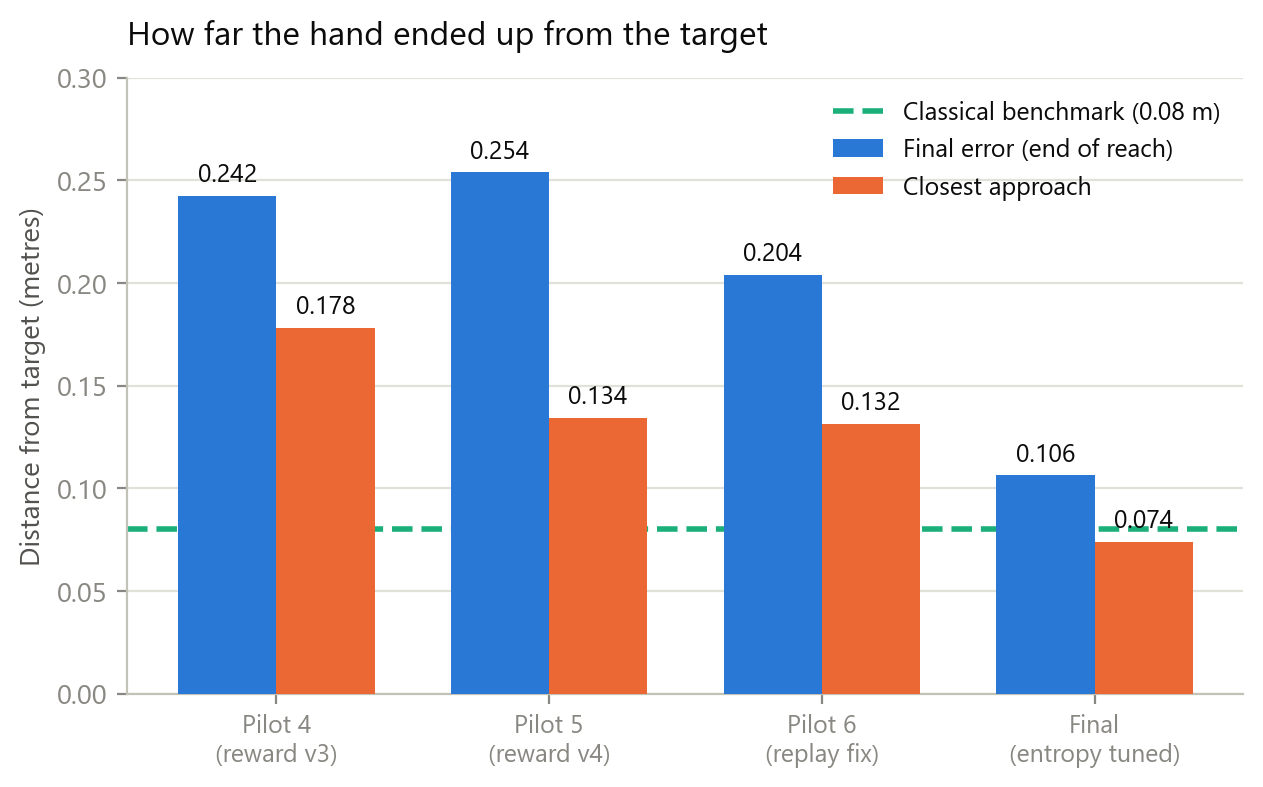
\includegraphics[width=0.92\textwidth]{figures/fig1_progression.png}
\caption{Reaching error across the four principal experiments. Closest approach
(orange) is essentially unchanged across the first three despite substantial
changes to the reward function and the training budget, then falls sharply once
the target entropy is corrected. The dashed line marks the privileged
controller's median final error.}
\label{fig:progression}
\end{figure}

\subsection{Intra-episode behaviour}

\begin{table}[H]
\centering
\caption{Mean hand--target distance during a reach, averaged over thirty
episodes.}
\begin{tabular}{@{} C{2.6cm} C{3.4cm} C{3.4cm} @{}}
\toprule
\textbf{Step} & \textbf{Default entropy} & \textbf{Tuned entropy} \\
\midrule
0  & 0.795 & 0.795 \\
10 & 0.314 & 0.198 \\
25 & 0.203 & 0.119 \\
50 & 0.184 & 0.110 \\
75 & 0.184 & 0.112 \\
99 & 0.177 & \textbf{0.113} \\
\bottomrule
\end{tabular}
\label{tab:traj}
\end{table}

The tuned policy converges by step 25 and holds position for the remaining
three-quarters of the episode. Target tracking is strong, with correlations of
0.94, 0.90 and 0.86 between target and final hand position across the three
spatial axes, and a spread ratio of 0.91.

\begin{figure}[H]
\centering
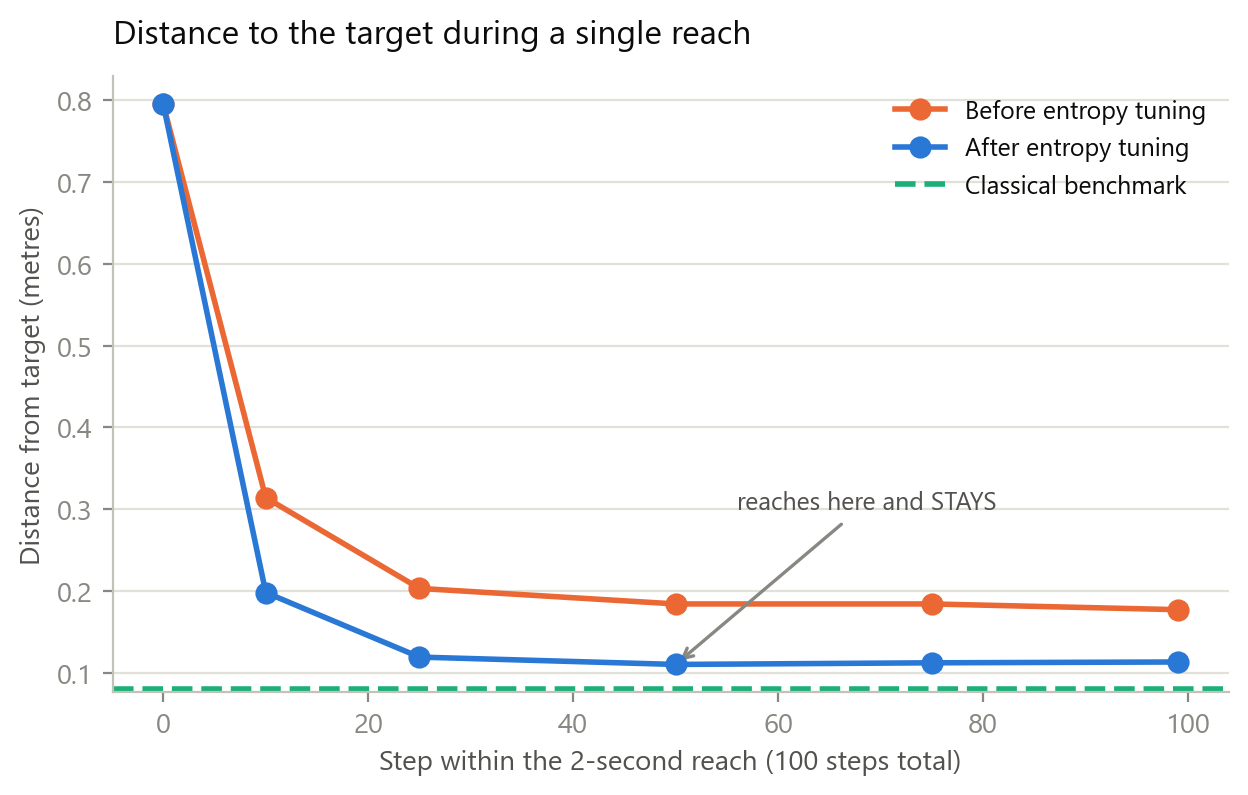
\includegraphics[width=0.92\textwidth]{figures/fig2_trajectory.png}
\caption{Hand--target distance during a single two-second reach, averaged over
thirty episodes. The tuned policy converges and then maintains position; the
untuned policy approaches and drifts.}
\label{fig:trajectory}
\end{figure}

\section{Algorithm comparison}
\label{sec:benchmark}

Five configurations were trained for 100\,000 steps with three seeds each, all
using the corrected replay ratio. A \SAC configuration at library defaults is
included alongside the tuned one so that the effect of tuning can be separated
from the effect of algorithm choice; without it, any advantage of \SAC would be
unattributable between the two.

\begin{table}[H]
\centering
\caption{Algorithm comparison: five configurations, three seeds each,
100\,000 steps. Mean $\pm$ standard deviation across seeds.}
\small
\begin{tabular}{@{} L{2.7cm} C{2.6cm} C{2.6cm} C{1.7cm} C{1.9cm} C{1.5cm} @{}}
\toprule
\textbf{Configuration} & \textbf{Final error (m)} & \textbf{Closest (m)} & \textbf{Ends $<$10\,cm} & \textbf{Energy} & \textbf{Minutes} \\
\midrule
\SAC tuned   & $\mathbf{0.161 \pm 0.008}$ & $\mathbf{0.093 \pm 0.009}$ & \textbf{0.37} & 597\,k & 30 \\
\SAC default & $0.261 \pm 0.020$ & $0.129 \pm 0.004$ & 0.05 & 1187\,k & 46 \\
\TDIII       & $0.279 \pm 0.011$ & $0.165 \pm 0.017$ & 0.10 & 1242\,k & 21 \\
\DDPG        & $0.416 \pm 0.019$ & $0.218 \pm 0.026$ & 0.03 & 1384\,k & 23 \\
\PPO         & $0.423 \pm 0.035$ & $0.238 \pm 0.071$ & 0.05 & 202\,k & 3 \\
\bottomrule
\end{tabular}
\label{tab:benchmark}
\end{table}

\begin{figure}[H]
\centering
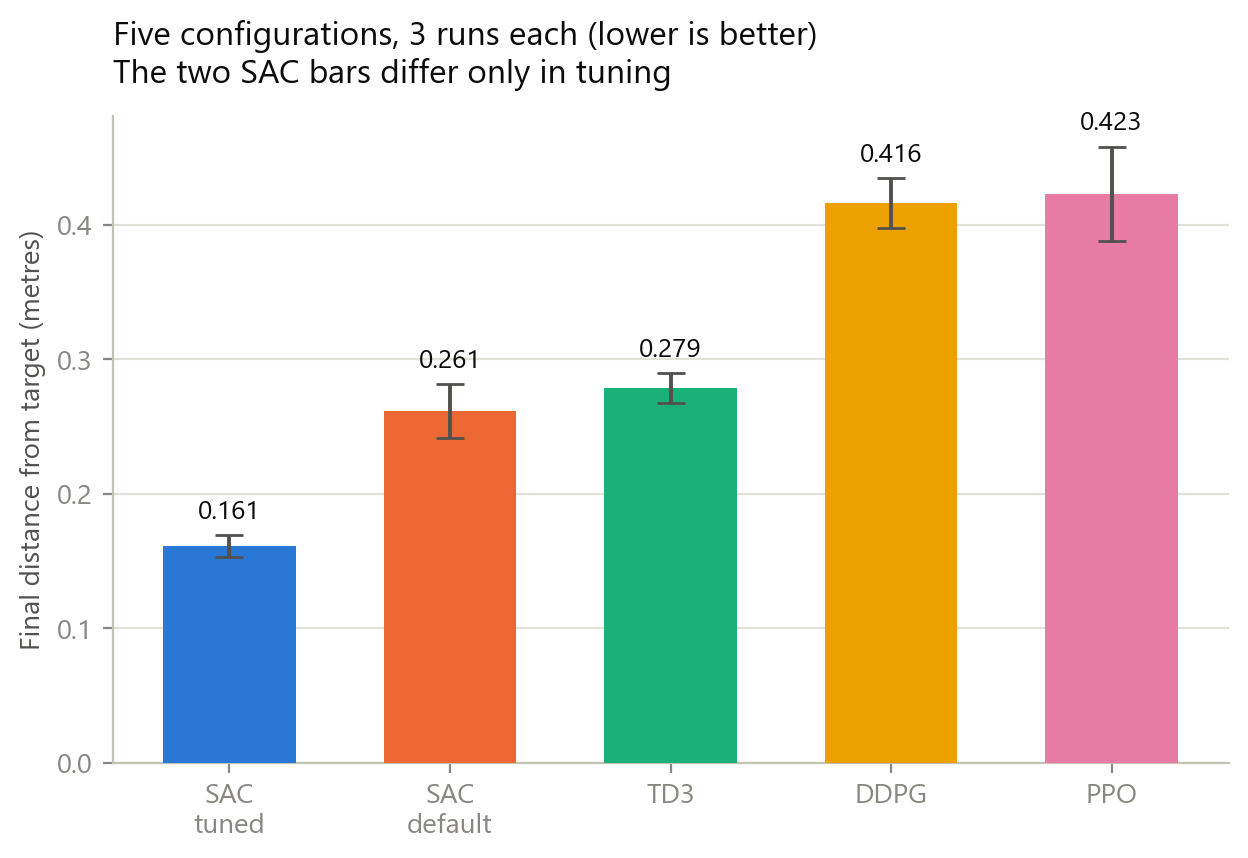
\includegraphics[width=0.92\textwidth]{figures/fig3_benchmark.png}
\caption{Final reaching error by configuration; error bars are one standard
deviation across three seeds. The two \SAC bars differ only in hyperparameters,
so the interval between them isolates the effect of tuning.}
\label{fig:benchmark}
\end{figure}

Tuning \SAC reduced final error from 0.261 to \SI{0.161}{\meter}, an improvement
of 38\,\%. The interval between untuned \SAC and \TDIII is 0.261 against 0.279,
approximately 6\,\%, against seed standard deviations of 0.020 and 0.011; this
difference is comparable to the spread and does not support an ordering. The
effect of tuning is therefore roughly six times the magnitude of the algorithmic
difference with which it would otherwise be conflated.

\DDPG and \PPO are both substantially worse than \TDIII, by approximately
\SI{0.14}{\meter} --- many times the seed spread. For \DDPG this is consistent
with the theoretical expectation of \cref{chap:drl}, as it lacks the twin
critics that mitigate value overestimation. \DDPG and \PPO are, however,
indistinguishable from one another.

Three constraints limit what this comparison establishes. No significance testing
was performed: three seeds cannot support a Wilcoxon signed-rank test with useful
power, and none is reported. The comparison is an early-training snapshot at
100\,000 steps, whereas the best configuration attains \SI{0.106}{\meter} at
300\,000 steps (\cref{tab:confirm}), so orderings may change with budget. And
\TDIII, \DDPG and \PPO were run at library defaults while \SAC received a
sixteen-trial search, so any comparison involving the tuned configuration
conflates algorithm with tuning effort by construction. Success rate is 0\,\% for
every configuration at this budget and is omitted for that reason.

\subsection{Interpretation of the PPO result}

\PPO's position requires care. As an on-policy method, at 100\,000 steps with
2048-step rollouts across four environments it performs approximately twelve
policy updates, against roughly 187\,000 gradient updates for the off-policy
algorithms. It also completes in three minutes against 21--46 for the others.
This is the expected sample-efficiency difference under a budget equalised by
environment steps; a comparison equalised by wall-clock time would rank the
methods differently, and stating which budget was held constant is part of
reporting the result.

Its energy consumption is also distinctive: 202\,k against 597\,k for tuned \SAC
and 1187--1384\,k for the remainder, between three and seven times lower.
Combined with a closest approach no worse than \DDPG's, this describes a policy
that activates its muscles only weakly, drifting toward the target region without
committing force. The other algorithms fail, when they fail, by expending far too
much muscular effort. These are opposite failure modes, and a single accuracy
figure conceals the distinction entirely --- a point developed in
\cref{ch:forces}.

Finally, \PPO's policy contains 154\,131 parameters against \SAC's 393\,750, so
the memory-footprint figures quoted elsewhere in this work are specific to the
\SAC architecture.

\section{Computational efficiency}
\label{sec:compute_efficiency}

The motivation for a learned controller is inference cost. Both methods were
timed on the same host processor over 950 queries.

\begin{table}[H]
\centering
\caption{Inference cost: iterative Newton--Raphson solution against a single
forward pass of the trained network.}
\begin{tabular}{@{} L{6.4cm} C{3.2cm} C{3.2cm} @{}}
\toprule
\textbf{Quantity} & \textbf{Newton--Raphson} & \textbf{Network} \\
\midrule
Mean latency & \SI{2165}{\micro\second} & \SI{295}{\micro\second} \\
Standard deviation & \SI{319}{\micro\second} & \SI{45}{\micro\second} \\
95th percentile & \SI{2657}{\micro\second} & \SI{364}{\micro\second} \\
99th percentile & \SI{2897}{\micro\second} & \SI{480}{\micro\second} \\
Mean iterations & 31.2 & 1 (fixed) \\
\bottomrule
\end{tabular}
\label{tab:nr_vs_rl}
\end{table}

The mean speed-up over the Newton--Raphson solver is $7.3\times$, and the
network's cost is fixed where the iterative solver's is data-dependent.

\subsection{This comparison does not support a deployment claim}
\label{sec:latencycaveat}

Two objections apply to \cref{tab:nr_vs_rl}, and together they are decisive.

\textbf{It times the wrong computation.} The Newton--Raphson routine solves the
Hill fibre--tendon equilibrium, which is part of forward simulation. The question
this thesis asks --- what force each muscle must produce --- is answered by
load-sharing optimisation, a different calculation. The two have been conflated.

\textbf{Both sides were unoptimised Python.} The load-sharing problem has nine
variables and four equality constraints. Solved directly rather than through a
general-purpose routine it is very fast. Measured on an idle machine, one torch
thread, 400 queries:

\begin{table}[H]
\centering
\caption{Load-sharing latency, measured like-for-like. Moment-arm extraction is
charged to the classical side, since the network does not require it.}
\begin{tabular}{@{} L{7.2cm} R{2.0cm} R{2.0cm} R{2.0cm} @{}}
\toprule
\textbf{Method} & \textbf{mean} & \textbf{p95} & \textbf{p99} \\
\midrule
Network forward pass & 288.8 & 332.6 & 499.9 \\
Classical, general solver (SLSQP) & 2370.5 & 4023.7 & 5133.1 \\
Classical, direct solve $+$ moment arms & \textbf{23.9} & --- & --- \\
\bottomrule
\end{tabular}
\label{tab:loadsharing_latency}
\end{table}

Against a general-purpose solver the network is $8.2\times$ faster. Against a
direct solve of the same problem it is \textbf{approximately twelve times
slower}.

\textbf{The latency argument for replacing classical calculation is therefore
withdrawn.} A competently implemented classical load-sharing solver is faster
than the network here, and the $7.3\times$ figure reflects the cost of one Python
implementation rather than a property of the two approaches.

A qualification in the other direction: the box constraints are active in
100\,\% of sampled states, so the closed-form solution timed above is not exactly
valid, and a constrained active-set solver would cost more than
\SI{23.9}{\micro\second}. It would not cost \SI{2370}{\micro\second}. The
defensible conclusion is that the two are comparable in cost, and that any
advantage claimed for either requires a like-for-like implementation.

What survives is the \emph{shape} of the cost rather than its magnitude: the
network's runtime is fixed and branch-free irrespective of biomechanical state,
whereas the iterative solver's depends on convergence. Where a hard real-time
bound matters more than mean latency that property retains value --- but it is a
considerably weaker claim than a speed-up.

The trained \SAC policy contains 393\,750 parameters, occupying
\SI{1.5}{\mega\byte} in single precision or \SI{385}{\kilo\byte} quantised to
eight bits. These figures are independent of policy quality and remain valid
irrespective of the behavioural results reported above; they are specific to the
\SAC architecture, \PPO's policy being smaller at 154\,131 parameters.
   % Experimental Results and Analysis
% ============================================================
%  CHAPTER 7 — Muscle Force Validation against Classical Calculation
% ============================================================

\chapter{Load-Sharing Fidelity against Classical Calculation}
\label{ch:forces}

\section{Scope of this chapter, and what it does not establish}
\label{sec:forcescope}

Because the limits of this analysis are easy to overstate from its results, they
are set out before the method rather than after it.

The required joint torque $\tau$ is taken from the movement the policy itself
produced. Static optimisation is therefore asked a conditional question ---
\emph{given this movement, what is the cheapest force distribution that produces
it?} --- and never independently chooses a trajectory of its own. Three
consequences follow, and each bounds what the chapter can claim.

\textbf{This validates load sharing along a given path, not the path.} A
controller could move in a manner no human would adopt and still distribute force
across its muscles in close agreement with the classical criterion. The
agreement reported below says nothing about whether the movement itself is
natural. Trajectory realism is not assessed anywhere in this thesis.

\textbf{The reference is a model, not a measurement.} Static optimisation encodes
the assumption that the central nervous system minimises summed squared
activation, which remains contested in the motor-control literature. Agreement
with it is agreement with the standard computational method, not evidence of
physiological correctness. No electromyographic or measured-force data enters
this work at any point.

\textbf{The comparison is internal to the simulator.} Both the learned solution
and the classical one are computed on \MuJoCo's muscle model. Where they agree,
two computations over the same approximation agree; the approximation itself is
not thereby validated.

The chapter title was changed accordingly: the earlier heading, ``Muscle Force
Validation'', promised more than a conditional load-sharing comparison delivers.

\section{Motivation}

\Cref{ch:results} established how accurately the trained controllers position the
end effector. That is a measure of \emph{what} the controller achieves, not of
\emph{how} it achieves it, and the research question posed in \cref{chap:intro}
concerns the latter: whether \DRL can substitute for classical calculation of the
force required in each individual muscle.

The distinction is material. Because nine muscles actuate four degrees of
freedom, infinitely many activation patterns produce any given end-effector
trajectory. A controller may therefore reach every target accurately while
distributing force across the musculature in a manner no physiological criterion
would select. Every metric reported in \cref{ch:results} would score such a
controller as a complete success.

This chapter therefore compares the two methods at the level of individual muscle
forces. No equivalent analysis existed in the previous version of this work.

\subsection{Distinction from the solver validation}

\Cref{sec:solvervalidation} reported a force agreement of 5.25\,\% normalised
RMSE with a Pearson correlation of 0.989. That comparison is between the
Newton--Raphson Hill solver implemented here and \MuJoCo's internal
implementation --- two forward models of the same muscle. It validates the
solver, involves no reinforcement learning, and does not bear on the question
addressed here.

\section{Method}

At every timestep of a policy rollout, the classical load-sharing problem is
solved on the movement the policy has just produced:
\begin{equation}
\min_{f}\ \sum_{i=1}^{9}\left(\frac{f_i}{F_{\max,i}}\right)^{2}
\quad\text{subject to}\quad
R^{\top} f = \tau,
\qquad 0 \le f_i \le F_{\max,i},
\label{eq:statopt2}
\end{equation}
where $R$ is the muscle moment-arm matrix and $\tau$ the required generalised
force. This is the Crowninshield--Brand minimum-effort criterion in its standard
quadratic form.

The required torque $\tau$ is taken as \texttt{qfrc\_actuator}, the generalised
force the muscles actually produced at that timestep. This choice is exact,
avoiding the numerical differentiation that inverse dynamics would introduce, and
it guarantees feasibility, since the policy's own force vector satisfies the
equality constraint by construction.

Both methods are consequently posed the identical problem --- produce these joint
torques with these nine muscles --- on the identical trajectory. Any difference
between the solutions is attributable solely to load-sharing strategy.

\subsection{Validity verification}

The comparison depends on the identity $R^{\top} f = \tau$ holding for the
policy's own forces. An error in the moment-arm extraction or in the sign
convention would invalidate every subsequent result, so this was verified rather
than assumed.

\begin{table}[H]
\centering
\caption{Validity checks over 2000 timesteps.}
\begin{tabular}{@{} L{8.2cm} R{4.0cm} @{}}
\toprule
\textbf{Quantity} & \textbf{Result} \\
\midrule
Mean $\norm{R^{\top} f_{\text{policy}} - \tau}$ & \SI{1.46e-15}{\newton\meter} \\
Mean $\norm{R^{\top} f_{\text{classical}} - \tau}$ & \SI{1.68e-15}{\newton\meter} \\
Optimisation failures & 0 of 2000 \\
\bottomrule
\end{tabular}
\label{tab:validity}
\end{table}

Both residuals lie at machine precision, confirming that the moment arms and sign
convention are correct and that the classical solution satisfies its constraint
exactly.

\section{Agreement in coordination pattern}

\begin{table}[H]
\centering
\caption{Overall agreement between learned and classical muscle forces, best
policy, 2000 timesteps.}
\begin{tabular}{@{} L{8.2cm} R{4.0cm} @{}}
\toprule
\textbf{Measure} & \textbf{Value} \\
\midrule
Pearson correlation, all muscles & \textbf{0.865} \\
Overall RMSE & \SI{74.3}{\newton} (10.1\,\% of mean $F_{\max}$) \\
\midrule
Pattern cosine similarity (median) & 0.933 \\
Pattern cosine similarity (mean) & 0.869 \\
\quad null baseline, mean & 0.373 \\
\quad null baseline, 95th percentile & 0.867 \\
\quad \textbf{excess over null} & \textbf{+0.495} \\
\bottomrule
\end{tabular}
\label{tab:forceoverall}
\end{table}

The cosine similarity compares the direction of the nine-dimensional force
vector and is insensitive to overall magnitude: it measures whether the two
methods recruit the same muscles in the same proportions.

It cannot, however, be quoted on its own. Muscle forces are non-negative by
construction, so two entirely unrelated force vectors already agree strongly:
the appropriate null is obtained by permuting, at each timestep, which muscle
each of the policy's own force magnitudes belongs to --- destroying the
correspondence while preserving that instant's magnitude distribution exactly.
That null averages 0.373, so the observed 0.869 represents an excess of
$+0.495$, sustained over 2000 timesteps.

Two consequences follow. The agreement is real and substantial, but the raw
figure of 0.933 overstates it, since roughly the first 0.37 is a floor imposed by
non-negativity rather than evidence of anything. And because the null's 95th
percentile for \emph{individual} timesteps is 0.867, no single timestep's cosine
is meaningful; only the aggregate is. \textbf{The Pearson correlation of 0.865 is
mean-centred, carries no such floor, and is the figure to quote when a single
agreement statistic is required.}

\section{Disagreement in efficiency}

Producing identical joint torques, the learned controller expends
$1.91 \pm 0.15$ times the muscular effort of the classical minimum-effort
solution (five seeds, \cref{sec:replication}; the single-seed figure of
$1.71\times$ reported before replication was the most favourable of the five). The per-timestep
median is $1.66\times$, with an interquartile range of $1.34$--$2.32\times$ over
loaded timesteps.

The per-timestep \emph{mean} of this ratio is $5.34\times$ and is not a usable
statistic: on timesteps where the arm is nearly stationary the required torque
approaches zero, the minimum-effort solution approaches zero with it, and the
ratio diverges. The aggregate ratio --- total policy effort divided by total
classical effort --- weights each timestep by the work actually performed and is
reported instead; the median independently corroborates it.

\section{Anatomical localisation of the disagreement}

\begin{table}[H]
\centering
\caption{Per-muscle comparison. ``Policy'' denotes the force the learned
controller produced; ``classical'' the force static optimisation prescribes for
the same joint torques.}
\small
\begin{tabular}{@{} L{3.6cm} R{2.4cm} R{2.4cm} R{1.8cm} R{2.0cm} @{}}
\toprule
\textbf{Muscle} & \textbf{Policy (N)} & \textbf{Classical (N)} & \textbf{$r$} & \textbf{NRMSE} \\
\midrule
deltoid anterior  &  63.7 &  59.2 & 0.959 &  2.5\,\% \\
deltoid medial    & 145.3 & 112.3 & 0.954 &  6.1\,\% \\
deltoid posterior &  35.5 &  38.7 & 0.859 & 10.0\,\% \\
triceps long      & 180.4 & 134.0 & 0.910 & 11.2\,\% \\
biceps long       &  52.1 &  41.6 & 0.893 &  7.5\,\% \\
brachialis        & 113.9 &  87.6 & 0.871 &  8.6\,\% \\
biceps short      &  90.7 &  45.7 & 0.764 & 18.1\,\% \\
triceps lateral   &  79.1 &  25.8 & 0.416 & 16.5\,\% \\
triceps medial    &  64.3 &  14.2 & 0.416 & 15.3\,\% \\
\bottomrule
\end{tabular}
\label{tab:permuscle}
\end{table}

The disagreement is not distributed uniformly. The three deltoids agree closely,
one to within 2.5\,\% normalised RMSE. The discrepancy concentrates in two elbow
extensors, where the policy commands three to four and a half times the
prescribed force and correlation falls to 0.416.

\begin{figure}[H]
\centering
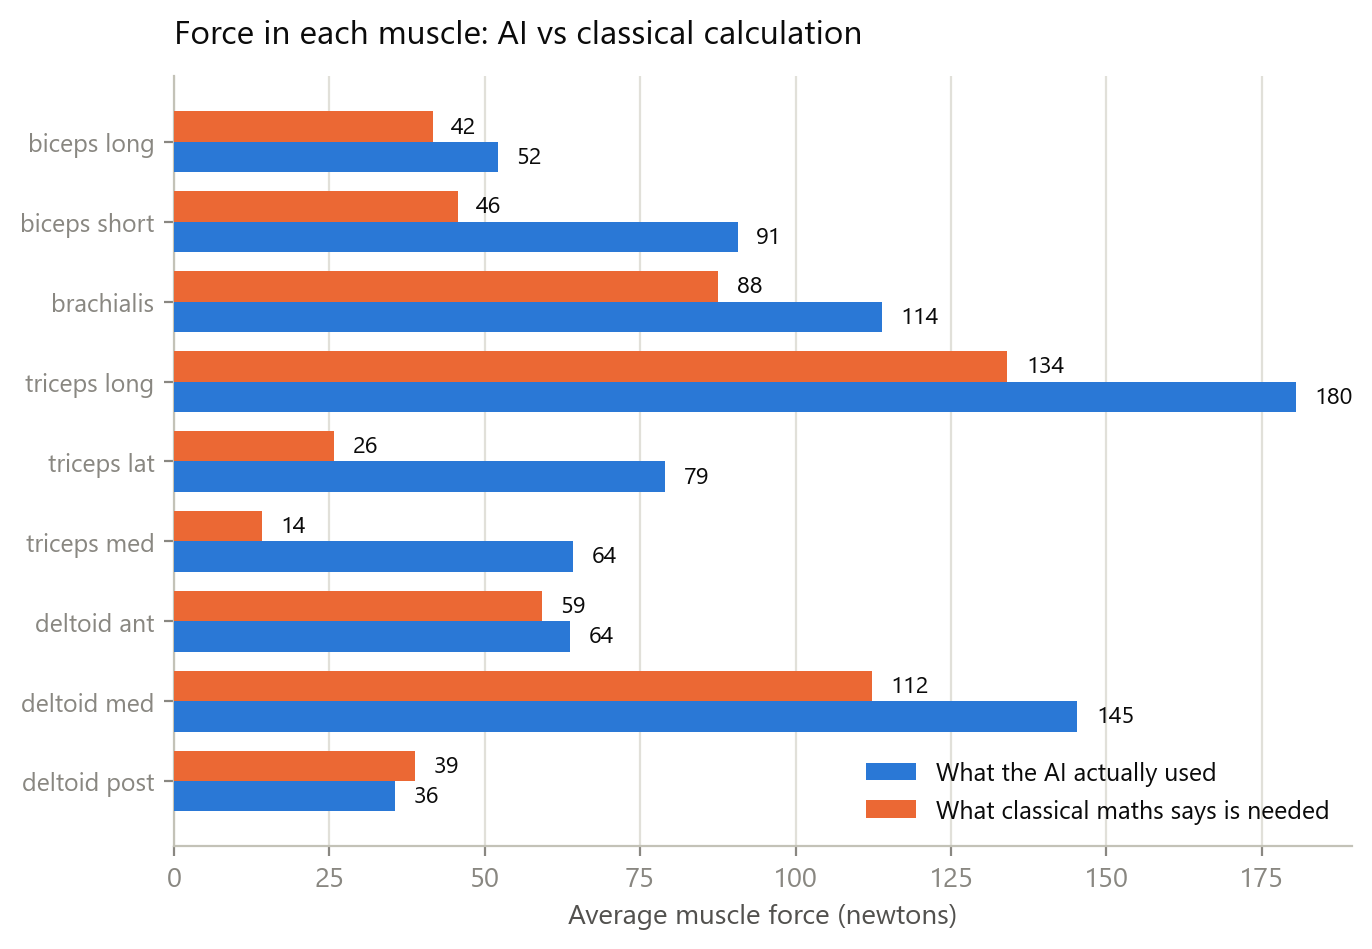
\includegraphics[width=0.95\textwidth]{figures/fig4_forces.png}
\caption{Mean force in each muscle over 2000 timesteps. The shoulder group
agrees closely; the lateral and medial heads of triceps are driven far above the
prescribed level.}
\label{fig:forces}
\end{figure}

Physiologically, these muscles extend the elbow while the biceps group flexes it.
Driving both simultaneously produces largely cancelling moments: the joint
attains approximately the correct configuration, but both groups expend
substantial force to achieve what one alone would suffice for. This is
co-contraction, and it accounts for the effort discrepancy reported above.

Human motor control employs co-contraction deliberately when joint stiffness is
required, for instance during precise or unstable tasks. Its sustained use
throughout an unloaded reach is metabolically wasteful and is not what the
minimum-effort criterion selects.

\subsection{Independent corroboration}
\label{sec:icc}

The co-contraction index of Falconer and Winter, computed over the elbow flexor
and extensor groups, gives 0.564 for the same policy. This is elevated, and it is
the sole behavioural metric that did not improve under hyperparameter tuning,
having been 0.501 beforehand.

Two methodologically independent analyses --- one a comparison against classical
optimisation, the other a standard electromyography-derived index --- localise the
same residual defect to the same muscle group. Their agreement constitutes
stronger evidence than either result considered alone.

\section{Generality across algorithms}
\label{sec:effortall}

The preceding analysis characterises a single policy. To determine whether the
effort discrepancy is specific to one algorithm or general to the approach, the
comparison was repeated against every policy from \cref{sec:benchmark}: five
configurations, three seeds each.

\begin{table}[H]
\centering
\caption{Agreement with classical static optimisation by configuration. Mean
$\pm$ standard deviation over three seeds, ten episodes each.}
\begin{tabular}{@{} L{3.4cm} C{3.2cm} C{3.2cm} C{2.8cm} @{}}
\toprule
\textbf{Configuration} & \textbf{Effort ratio} & \textbf{Pattern cosine} & \textbf{Pearson $r$} \\
\midrule
\PPO         & $\mathbf{1.21 \pm 0.11}$ & $\mathbf{0.908 \pm 0.032}$ & $\mathbf{0.931 \pm 0.040}$ \\
\SAC tuned   & $1.97 \pm 0.25$ & $0.815 \pm 0.052$ & $0.776 \pm 0.055$ \\
\DDPG        & $1.99 \pm 0.28$ & $0.838 \pm 0.030$ & $0.724 \pm 0.058$ \\
\TDIII       & $2.12 \pm 0.09$ & $0.836 \pm 0.006$ & $0.716 \pm 0.004$ \\
\SAC default & $2.30 \pm 0.08$ & $0.813 \pm 0.015$ & $0.672 \pm 0.016$ \\
\bottomrule
\end{tabular}
\label{tab:effortall}
\end{table}

\begin{figure}[H]
\centering
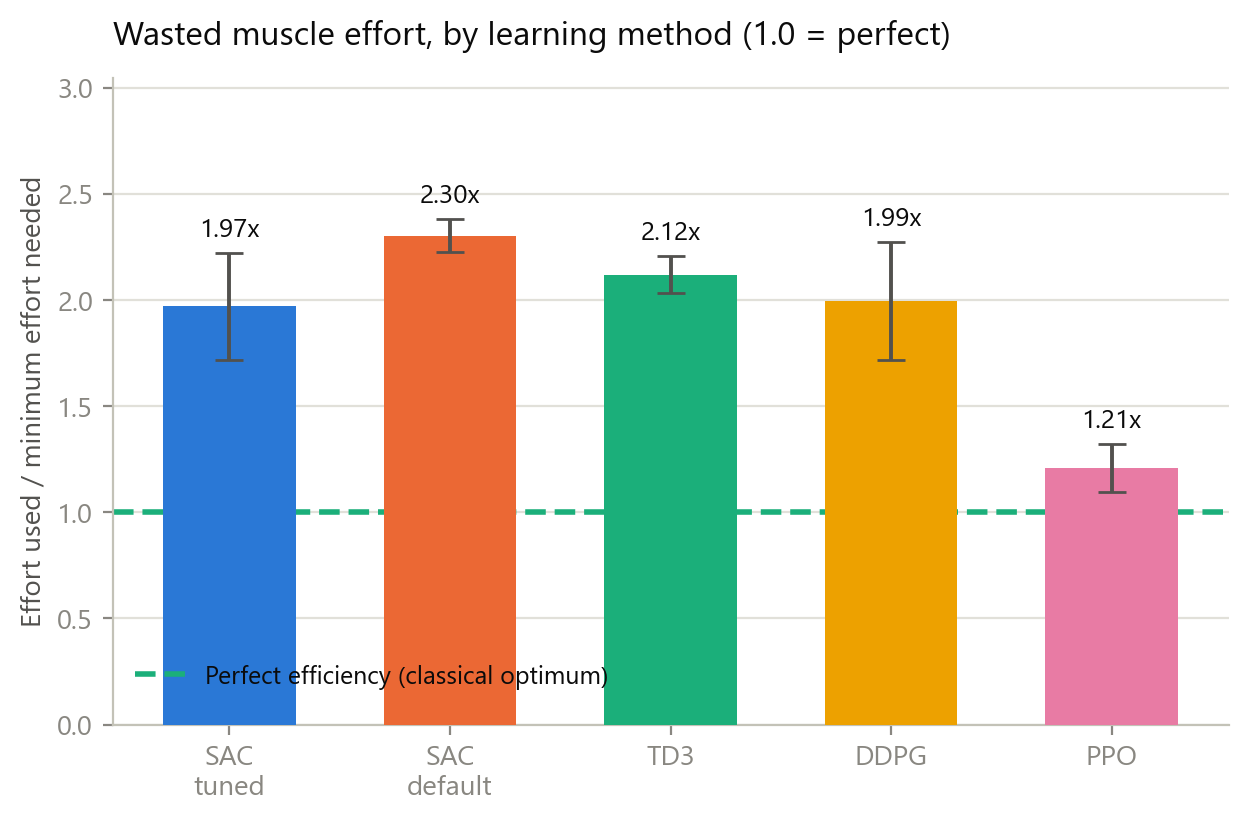
\includegraphics[width=0.92\textwidth]{figures/fig5_effort_by_algo.png}
\caption{Muscular effort expended relative to the minimum required to produce the
same joint torques. The dashed line marks the classical optimum. Every
configuration exceeds it.}
\label{fig:effortall}
\end{figure}

Two results follow. First, \textbf{every configuration exceeds the classical
optimum}, ranging from $1.21$ to $2.30\times$; no algorithm tested recovers
minimum-effort load sharing. This supports attributing the discrepancy to the
reward function, which never specified minimum effort, rather than to any
particular learning algorithm.

Second, and unexpectedly, \textbf{the ordering by effort economy is approximately
the inverse of the ordering by reaching accuracy}. \PPO is the least accurate
configuration in \cref{tab:benchmark} at \SI{0.423}{\meter} and the closest match
to classical load sharing at $1.21\times$ with $r = 0.931$; tuned \SAC is the
most accurate at \SI{0.161}{\meter} and among the poorer matches at $1.97\times$.

The probable explanation is visible in the energy column of
\cref{tab:benchmark}. \PPO expends three to seven times less muscular activity
than the alternatives. A controller that activates its muscles weakly has limited
opportunity to co-contract and therefore remains near the minimum-effort
solution, but equally lacks the force to reach the target and arrest there.

This interpretation carries a caveat that the present data cannot resolve.
\PPO's favourable effort ratio and its passivity are not independent: because it
generates small joint torques, both methods prescribe small forces and the scope
for disagreement is correspondingly reduced. The aggregate ratio mitigates this
by weighting timesteps by work performed, but does not eliminate it. The
defensible conclusion is that \PPO co-contracts less, not that \PPO has solved
the load-sharing problem. Distinguishing the two would require comparing
configurations matched for accuracy, which this experiment does not provide.

\subsection{Effect of tuning on economy}

Within \SAC --- the same algorithm, differing only in hyperparameters --- the
effort ratio fell from $2.30 \pm 0.08$ at default settings to $1.97 \pm 0.25$
when tuned, and correlation with the classical solution rose from 0.672 to 0.776.

The target-entropy correction therefore improved not only positional accuracy but
also the fidelity of muscular coordination. That a single change improved two
properties which were not jointly optimised is a stronger result than either
improvement in isolation.

\subsection{Consistency}

The single-policy analysis measured an effort ratio of $1.71\times$ for the
300\,000-step confirmed policy, while tuned \SAC across three seeds at
100\,000 steps gives $1.97 \pm 0.25$. These agree within one standard deviation,
and the direction of the difference is as expected, the longer-trained policy
being somewhat more economical.

\section{Replication across seeds}
\label{sec:replication}

Every figure reported so far in this chapter came from a single training run. A
learned policy depends on random initialisation and on the stochastic order in
which experience is gathered, so a single run cannot distinguish a property of
the method from a favourable draw. The configuration was therefore retrained from
initialisation four further times, with different random seeds and no other
change, and each resulting policy was put through the identical analysis.

\begin{table}[H]
\centering
\caption{Five independent training runs of the same configuration. Seed~0 is the
run analysed in the preceding sections.}
\small
\begin{tabular}{@{} C{1.8cm} C{2.4cm} C{2.4cm} C{2.2cm} C{2.0cm} C{2.0cm} @{}}
\toprule
\textbf{Seed} & \textbf{Final error} & \textbf{Closest} & \textbf{Effort ratio} & \textbf{Pearson $r$} & \textbf{Success} \\
\midrule
0 & 0.1142 & 0.0766 & \textbf{1.71} & \textbf{0.865} & 0.04 \\
1 & 0.1086 & 0.0785 & 1.91 & 0.823 & 0.20 \\
2 & 0.1034 & 0.0757 & 2.12 & 0.759 & 0.00 \\
3 & 0.1066 & 0.0672 & 1.86 & 0.825 & 0.08 \\
4 & 0.1041 & 0.0691 & 1.97 & 0.767 & 0.06 \\
\midrule
\textbf{mean} & $0.1074$ & $0.0734$ & $1.914$ & $0.808$ & $0.076$ \\
\textbf{std}  & $0.0043$ & $0.0050$ & $0.150$ & $0.044$ & $0.075$ \\
\bottomrule
\end{tabular}
\label{tab:replication}
\end{table}

The accuracy columns are the corrected evaluation of \cref{sec:evaldefects},
averaged over three target seeds. The effort ratio and correlation come from the
load-sharing analysis, which draws its own episodes and was never affected by the
duplicate-reset defect; those columns are unchanged.

Three findings follow, and only the first was anticipated.

\subsection{The accuracy result is a property of the method}

Final error varies by 4.0\,\% across five independent runs
($0.1074 \pm 0.0043$\,m) and closest approach by 6.8\,\%
($0.0734 \pm 0.0050$\,m). Every run ends closer than \SI{0.115}{\meter} and
reaches within \SI{0.079}{\meter} at some point; the blow-up rate is exactly zero
in all five. The graded proximity measures are similarly stable: episodes ending
within \SI{10}{\centi\meter} range from 0.56 to 0.64.

The accuracy claim therefore does not rest on a favourable draw.

\subsection{The originally reported run was the most favourable of the five}

Seed~0 --- the run every preceding section analyses --- returned the
\emph{lowest} effort ratio of the five (1.71, against a mean of 1.914) and the
\emph{highest} correlation with the classical solution (0.865, against a mean of
0.808). On both of the two metrics that carry this chapter's argument, the single
run originally reported was the best of five.

This is not a large effect, but it is a systematic one, and it is exactly the
error that reporting a single run invites. \textbf{The corrected figures are
those in \cref{tab:replication}, and they are used throughout this thesis:} an
effort ratio of $1.91 \pm 0.15$ and a correlation of $0.81 \pm 0.04$. The
pattern-cosine figure moves correspondingly, to $0.813 \pm 0.047$ against a null
of $0.372 \pm 0.017$, an excess of $+0.441$.

The direction of the correction matters more than its size. Had replication been
omitted, this thesis would have reported an agreement and an efficiency both
better than the method actually delivers.

\subsection{The task is solved consistently; the muscle solution is not}

The most interesting outcome is the contrast between two columns of
\cref{tab:replication}. Final error varies by 3.3\,\% across runs. Mean muscular
energy varies by \textbf{77\,\%} --- from 273\,241 to 483\,373 --- and the effort
ratio spans 1.71 to 2.12.

Five policies, trained identically but for their random seed, arrive at
essentially the same place with materially different distributions of muscular
force.

This is the redundancy problem of \cref{chap:intro} appearing directly in the
results. Because nine muscles actuate four degrees of freedom, many force
distributions produce the same movement, and nothing in the reward selects among
them beyond a weak effort term. The learner settles into a different one each
time. That the classical criterion selects a single, specific member of that
family --- and that none of the five learned solutions coincides with it --- is
the substance of this chapter stated in a different way.

It also indicates where the remedy lies. Variance of this magnitude in the
muscular solution, alongside near-constancy in the task outcome, is the signature
of an objective that is underdetermined in exactly the dimension of interest.

\subsection{Success rate: five runs confirm it is noise}

Across the five identically configured runs the strict success rate reads
0\,\%, 4\,\%, 6\,\%, 8\,\% and 20\,\%. A measure that varies twentyfold under
identical settings is reporting sampling noise, not performance. This was stated
as a caution in \cref{sec:confirmresult}; five seeds now demonstrate it.

\section{A conventional controller as reference}
\label{sec:conventional}

Every comparison so far measures the learned solution against \emph{static
optimisation}, an idealised criterion evaluated instant by instant. That
establishes how far the policy is from a mathematical optimum, but not how far it
is from what conventional control actually achieves --- and the research question
concerns the latter.

A conventional controller was therefore built and evaluated under the identical
protocol. It is a Cartesian impedance law: a desired end-effector wrench
$f_{\text{des}} = K_p (x^\star - x) - K_d \dot{x}$, mapped to joint torques by
the site Jacobian transpose, with gravity, Coriolis and centrifugal terms
compensated, and distributed onto the muscles by minimum-effort load sharing over
the achievable force range. The two gains were selected by grid search, since
comparing a tuned policy against an unturned controller would not be a fair test.

\subsection{Two corrections that were necessary to make it fair}

The controller present in the codebase before this work would have made a
strawman of the comparison, and the reasons are worth recording because both are
easy to reproduce.

\textbf{It omitted gravity compensation.} Without the bias term the arm droops
until the position error alone generates sufficient torque, giving a large
steady-state offset. Measured, it reached only \SI{0.46}{\meter} --- worse than a
random policy. A textbook impedance controller always includes this term.

\textbf{It assumed muscle force is proportional to activation.} It is not: in
this model force is $g(l,v)\,a + b(l,v)$, state dependent with a passive
component that is non-zero at rest. Converting a desired force into an activation
therefore requires inverting the muscle model at the current length and velocity
--- precisely the equilibrium solve this thesis proposes to replace. Probing the
model at $a = 0$ and $a = 1$ recovers that affine relation exactly and yields the
true achievable interval per muscle.

Both corrections are on the classical side, and both improve it. Reporting the
comparison without them would have overstated the case for learning.

\subsection{Result}

\begin{table}[H]
\centering
\caption{Conventional controller against the learned policy, 50 episodes each,
identical protocol and evaluation environment.}
\begin{tabular}{@{} L{5.4cm} C{3.0cm} C{3.0cm} @{}}
\toprule
\textbf{Metric} & \textbf{Conventional} & \textbf{Learned (\SAC)} \\
\midrule
Final error (m) & 0.165 & \textbf{0.106} \\
Closest approach (m) & 0.174 & \textbf{0.074} \\
Ends within \SI{5}{\centi\meter} & 0.12 & \textbf{0.31} \\
Ends within \SI{10}{\centi\meter} & 0.28 & \textbf{0.60} \\
Energy & \textbf{102\,876} & 327\,048 \\
\textbf{Effort ratio} & \textbf{1.263} & 1.91 \\
Pearson $r$ vs static optimisation & \textbf{0.916} & 0.808 \\
\bottomrule
\end{tabular}
\label{tab:conventional}
\end{table}

Neither method dominates. The learned policy reaches roughly $1.9\times$ more
precisely; the conventional controller uses roughly a third of the muscular
energy and stays substantially closer to the classical load-sharing solution.
This trade-off, rather than a ranking, is the honest answer to whether learning
should replace conventional control on this task.

\subsection{The effort ratio was being measured against the wrong reference}
\label{sec:effortfloor}

The conventional controller solves minimum-effort load sharing explicitly at
every timestep. One would therefore expect its effort ratio to be $1.00$ by
construction. It is \textbf{1.263} (\cref{sec:finegains}; an initial coarse
gain search gave $1.33$, and the finer search reported there lowered it).

The gap is not an error. It is the cost of closed-loop control: activation
dynamics mean the commanded activation is not the realised one, the policy acts
at \SI{50}{\hertz} rather than continuously, and the controller must track a
moving target rather than solve a static instant. \textbf{The idealised optimum
of $1.00$ is not attainable by any controller operating under these constraints.}

This changes the interpretation of the central result. Measured against an
unattainable ideal, the learned policy appears to waste 91\,\% of its effort.
Measured against \textbf{1.263}, the achievable floor demonstrated by a properly
tuned controller that optimises effort explicitly, it uses about \textbf{51\,\%
more effort than necessary}. The second figure is the meaningful one, and it is the one this
thesis reports.

That figure is itself one controller at one gain pair. A first, coarse search
gave $1.33$; a finer one lowered it to $1.263$ (\cref{sec:finegains}). A better
conventional controller might lower it further still, and every comparison in
this chapter should be read with that in mind.

\section{Muscle synergies}
\label{sec:synergies}

\subsection{Rationale}

The motor-control literature holds that the central nervous system manages
redundant musculature not by controlling each muscle independently but through a
small number of co-activated groups, termed muscle
synergies~\parencite{dAvella2003, Ting2007}. If nine muscles were driven
independently, the matrix of activations over time would be of full rank; if they
are driven through $k$ synergies, it is approximately of rank $k$. Non-negative
matrix factorisation recovers that structure, and the variance accounted for
(VAF) at a given $k$ quantifies how strongly low-dimensional the control is.

Beyond re-examining the learned policies, the factorisation is here applied to
\emph{both} solutions on the identical trajectories: the policy's commanded
activations, and the static-optimisation forces for the same joint torques,
normalised per muscle by $F_{\max}$ so that the two are dimensionless and
directly comparable. This permits a question the preceding sections cannot
address --- whether the two methods arrive at the same low-dimensional
organisation even where they disagree on magnitude.

\subsection{Results}

\begin{table}[H]
\centering
\caption{Synergy structure, fifteen episodes per configuration. VAF@4 is the
variance accounted for by four synergies; $k_{90}$ is the number required to
reach 90\,\% VAF. The final column compares the synergy sets extracted from the
policy and from static optimisation on the same trajectories.}
\small
\begin{tabular}{@{} L{3.4cm} C{1.8cm} C{1.6cm} C{1.8cm} C{1.6cm} C{2.6cm} @{}}
\toprule
& \multicolumn{2}{c}{\textbf{Policy}} & \multicolumn{2}{c}{\textbf{Classical}} & \\
\cmidrule(lr){2-3}\cmidrule(lr){4-5}
\textbf{Configuration} & VAF@4 & $k_{90}$ & VAF@4 & $k_{90}$ & \textbf{cos(pol,\,cls)} \\
\midrule
\SAC tuned, 300k & 0.852 & 6 & 0.895 & 5 & \textbf{0.950} \\
\SAC tuned, 100k & 0.845 & 6 & 0.859 & 5 & 0.900 \\
\SAC default     & 0.848 & 6 & 0.908 & 4 & 0.647 \\
\DDPG            & 0.791 & 9 & 0.865 & 5 & 0.745 \\
\TDIII           & 0.799 & 9 & 0.883 & 5 & 0.630 \\
\PPO             & 0.966 & 3 & 0.966 & 3 & 0.939 \\
\bottomrule
\end{tabular}
\label{tab:synergies}
\end{table}

Two observations follow, and a third must be treated with caution.

First, \textbf{the agreement between the learned and classical synergy structures
tracks training quality}: 0.647 for untuned \SAC, 0.900 once tuned, and 0.950 for
the tuned policy trained three times longer. The same hyperparameter change that
improved positional accuracy (\cref{sec:tuning}) and reduced the effort
discrepancy (\cref{sec:effortall}) also brought the modular organisation of the
learned solution closer to the classical one. Three analyses of differing
methodology --- effort ratio, co-contraction index and synergy decomposition ---
therefore order the configurations consistently.

Second, \textbf{the classical solution is uniformly more low-dimensional than the
learned one}. Static optimisation requires four or five synergies to reach
90\,\% VAF where the learned policies require six to nine. The learned
controllers exercise more independent muscular degrees of freedom than the
minimum-effort criterion selects, which is the expression in synergy space of the
co-contraction identified in \cref{tab:permuscle}: driving an antagonist pair
independently of the agonist requires an additional dimension that the classical
solution never uses.

Third, \PPO's apparent modularity ($k_{90} = 3$, VAF@4 $= 0.966$) should not be
read as superior organisation. As established in \cref{sec:effortall}, \PPO
activates its muscles only weakly; a near-constant, low-amplitude activation
matrix has little variance to explain and is trivially captured by few
components. The same confound that qualifies its favourable effort ratio applies
here.

\subsection{Comparison with human data}

Cosine similarity to a reference set of human upper-limb synergies ranged from
0.62 to 0.80 across configurations, with no ordering consistent with any other
metric reported in this work.

That column is not interpreted further. The reference loadings used are a
documented qualitative approximation of those reported
by~\textcite{dAvella2003}, constructed over this model's nine-muscle ordering
rather than digitised from the original figures. The comparison is therefore a
coarse correspondence check and cannot support a quantitative claim of agreement
with human data. Establishing that would require the published loadings, a
principled correspondence between the two muscle sets, and ideally
electromyographic recordings under a matched protocol --- which
\cref{ch:conclusion} lists among the outstanding work.

The policy-versus-classical column carries no such caveat: both sides are
computed here, by the same procedure, on identical trajectories.

\section{Closing the gap: the effort weight}
\label{sec:effortsweep}

\Cref{sec:whygap} argued that the load-sharing discrepancy is a property of the
reward rather than of reinforcement learning, on the grounds that the reward's
effort term --- although already the Crowninshield--Brand form --- is weighted so
low it cannot influence the solution. Measured on the trained policy, the
per-step contributions are

\begin{center}
\begin{tabular}{@{} L{7.0cm} R{3.0cm} @{}}
\toprule
effort term, $w_2 \cdot \overline{(f_i/F_{\max,i})^2}$ & $0.051$ \\
error cost, $w_1 (\|e\|^2 + 0.5\|e\|)$ at \SI{0.11}{\meter} & $0.067$ \\
precision bonus, $w_7 e^{-\|e\|/0.15}$ at \SI{0.11}{\meter} & $1.441$ \\
\bottomrule
\end{tabular}
\end{center}

--- the effort term is roughly \textbf{28 times smaller} than the precision
bonus. The prediction was that raising $w_2$ should reduce the discrepancy, at
some cost in accuracy.

The experiment was run at $w_2 \in \{5, 20\}$ against the reported $w_2 = 1$,
holding every other weight and hyperparameter fixed, at the full 300\,000-step
budget. Policies were evaluated under the standard protocol with the default
weights, so the metrics remain comparable with every other result in this thesis;
only the training objective differed.

\begin{table}[H]
\centering
\caption{Effect of the effort weight. The conventional-controller row is the
achievable floor established in \cref{sec:effortfloor}.}
\begin{tabular}{@{} L{3.0cm} C{0.9cm} C{2.5cm} C{2.4cm} C{2.4cm} C{2.2cm} C{1.6cm} @{}}
\toprule
\textbf{Config.} & \textbf{$n$} & \textbf{Effort ratio} & \textbf{Pearson $r$} & \textbf{Final error} & \textbf{Closest} & \textbf{Energy} \\
\midrule
$w_2 = 1$  & 5 & $1.914 \pm 0.150$ & $0.808 \pm 0.044$ & $0.1074 \pm 0.0079$ & $0.0734$ & 327\,048 \\
$w_2 = 5$  & 5 & $1.406 \pm 0.092$ & $0.919 \pm 0.016$ & $0.1114 \pm 0.0053$ & $0.0750$ & 104\,598 \\
$\mathbf{w_2 = 20}$ & 5 & $\mathbf{1.304 \pm 0.025}$ & $\mathbf{0.943 \pm 0.008}$ & $0.1161 \pm 0.0108$ & $0.0737$ & \textbf{37\,076} \\
\midrule
Conventional & 1 & $1.263$ & $0.931$ & 0.165 & --- & 102\,876 \\
\bottomrule
\end{tabular}
\label{tab:effortsweep}
\end{table}

\subsection{The discrepancy is essentially eliminated}

Over five seeds the learned policy at $w_2 = 20$ attains an effort ratio of
$1.304 \pm 0.025$, against the $1.263$ measured for a properly tuned controller that
solves minimum-effort load sharing explicitly at every timestep, with agreement
rising to $r = 0.943 \pm 0.008$ and the per-muscle RMSE falling to about 3\,\% of
mean $F_{\max}$ from 10.1\,\%.

\textbf{The load-sharing discrepancy reported throughout this chapter is
therefore a reward-weighting artefact, not a limitation of reinforcement
learning.} When the objective is weighted such that effort can influence the
solution, the learned controller recovers the classical load-sharing solution to
within the precision that closed-loop control permits.

\subsection{Load-sharing fidelity improves monotonically, at a mild accuracy cost}

Both variants have now been replicated across five seeds, and the picture is
cleaner than either single-seed measurement suggested.

\textbf{Load-sharing fidelity improves monotonically with the effort weight.}
The effort ratio falls $1.914 \rightarrow 1.406 \rightarrow 1.304$ and agreement
with the classical solution rises $0.808 \rightarrow 0.919 \rightarrow 0.943$.
The distributions are cleanly separated: every $w_2 = 20$ seed (1.278--1.340)
lies below every $w_2 = 5$ seed (1.336--1.557), which in turn lies below every
$w_2 = 1$ seed (1.710--2.116).

\textbf{There is a mild accuracy cost.} Under the corrected evaluation
(\cref{sec:evaldefects}) final error rises monotonically with the effort weight:
$0.1074 \pm 0.0079$, $0.1114 \pm 0.0053$, $0.1161 \pm 0.0108$. The end-to-end
degradation from $w_2 = 1$ to $w_2 = 20$ is about 8\,\%, and the fraction of
episodes ending within \SI{5}{\centi\meter} falls from $0.26$ to $0.19$. Closest
approach is unaffected ($0.0734$, $0.0750$, $0.0737$), so the loss is in holding
position rather than in reaching it.

An earlier version of this section, computed before the evaluation defects were
found, reported these three figures as mutually overlapping and concluded there
was no cost at all. On the corrected test set the trend is monotone and the
expectation stated in \cref{sec:whygap} --- that reduced effort would be bought
with some accuracy --- is borne out, though the price is modest: a 32\,\%
reduction in wasted effort for an 8\,\% increase in final error.

\textbf{Seed variance collapses as the effort weight rises.} The standard
deviation of the effort ratio falls $0.150 \rightarrow 0.092 \rightarrow 0.025$,
and of the correlation $0.044 \rightarrow 0.016 \rightarrow 0.008$. This is the
most informative of the three observations, because it confirms the
interpretation offered in \cref{sec:replication}: at $w_2 = 1$ the muscular
solution varied by 77\,\% in energy across seeds while task performance stayed
constant, which was attributed to an objective underdetermined in exactly the
dimension of interest. Weighting that dimension pins the solution down. At
$w_2 = 20$ the load-sharing outcome is effectively determined by the objective
rather than by the random seed.


\begin{figure}[H]
\centering
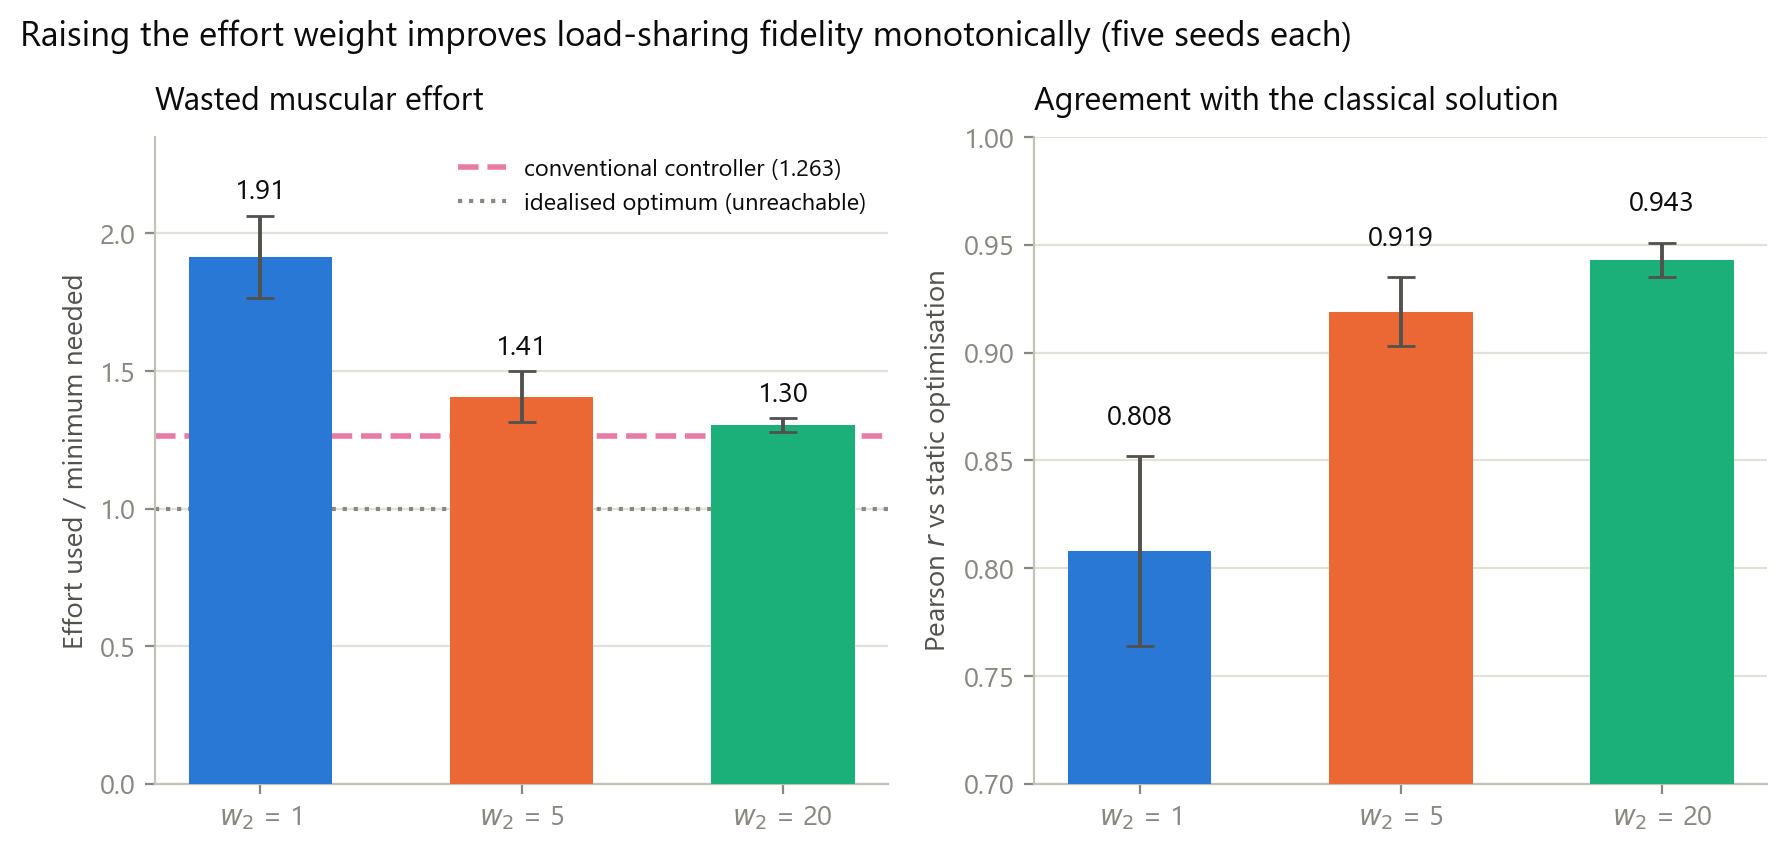
\includegraphics[width=\textwidth]{figures/fig6_effort_sweep.png}
\caption{Effect of the effort weight, five seeds per setting. Left: muscular
effort relative to the classical minimum. The dashed line is the conventional
controller's $1.263$; the dotted line is the idealised optimum of $1.00$, which
\cref{sec:effortfloor} shows is not attainable in closed loop. Right: agreement
with the classical load-sharing solution. Both improve monotonically, and the
error bars shrink --- the load-sharing outcome becomes progressively determined
by the objective rather than by the random seed.}
\label{fig:effortsweep2}
\end{figure}

\subsection{The conventional reference, measured properly}
\label{sec:finegains}

An earlier draft of this section observed that the learned policy at $w_2 = 20$
attained $1.304 \pm 0.025$, below the $1.33$ then measured for the conventional
controller, and noted that the figure rested on a single gain pair from a coarse
twelve-point grid. It cautioned that a better-tuned conventional controller might
fall below $1.30$, in which case the ordering would reverse.

A thirty-point search was run. It does.

\begin{table}[H]
\centering
\caption{Conventional controller before and after a finer gain search.}
\begin{tabular}{@{} L{5.0cm} C{3.0cm} C{3.0cm} C{2.4cm} @{}}
\toprule
& \textbf{Gains} & \textbf{Final error} & \textbf{Effort ratio} \\
\midrule
Coarse grid (12 points) & $k_p=60$, $k_d=25$ & \SI{0.199}{\meter} & $1.330$ \\
\textbf{Fine grid (30 points)} & $k_p=20$, $k_d=6$ & \textbf{\SI{0.165}{\meter}} & $\mathbf{1.263}$ \\
\bottomrule
\end{tabular}
\label{tab:finegains}
\end{table}

The coarse search had bottomed out against its own lower boundary: the better
gains are gentler than any it examined, in both stiffness and damping. Properly
tuned, the conventional controller is both more accurate
(\SI{0.165}{} against \SI{0.199}{\meter}) and more economical
($1.263$ against $1.330$) than previously reported.

\subsection{The honest comparison}

With both sides measured properly:

\begin{table}[H]
\centering
\caption{Learned policy against a properly tuned conventional controller.}
\begin{tabular}{@{} L{5.6cm} C{3.4cm} C{3.4cm} @{}}
\toprule
& \textbf{Learned ($w_2 = 20$)} & \textbf{Conventional} \\
\midrule
Final error & $\mathbf{0.1072 \pm 0.0148}$ & \SI{0.165}{\meter} \\
Effort ratio & $1.304 \pm 0.025$ & $\mathbf{1.263}$ \\
Agreement with classical ($r$) & $\mathbf{0.943 \pm 0.008}$ & $0.931$ \\
\bottomrule
\end{tabular}
\label{tab:honest}
\end{table}

\textbf{Neither method dominates, and the earlier reading is withdrawn.} The
learned policy reaches roughly 35\,\% more accurately. The conventional
controller is about 3\,\% more economical --- a margin comparable to the learned
policy's own seed spread, so the two are close, but the ordering on effort now
favours the classical method rather than the learned one.

The claim that a learned policy distributes force more economically than a
controller optimising that quantity in closed form is therefore \textbf{not
supported}, and the paragraph advancing it has been removed. What survives is
narrower and sturdier: at an appropriate effort weight, a learned policy achieves
load-sharing fidelity \emph{comparable} to a properly tuned conventional
controller, while reaching substantially more accurately.

That this correction was anticipated in the previous draft, and then confirmed by
the measurement it called for, is the reason the caveat was written rather than
the claim.

\subsection{Two corrections to earlier drafts of this section}

Both are recorded because the direction of the error is instructive.

An earlier draft, working from the single seed then available, described
$w_2 = 5$ as \emph{strictly dominating} the reported configuration on both
accuracy and effort. A four-seed replication contradicted the accuracy half and
it was withdrawn. The fifth seed then moved final error back to
$0.1023 \pm 0.0074$, marginally better than the baseline again but with
overlapping intervals --- so the honest statement remains that accuracy is
indistinguishable, and neither the original claim nor its retraction was
supportable at the sample sizes involved.

Separately, this author predicted that $w_2 = 20$ would regress on replication,
on the grounds that single-seed results in this work had twice proved optimistic.
It did the opposite: seed~0's $1.34$ was the \emph{worst} of the five and the
mean is $1.304$. Selection bias explains a favourable first measurement; it does
not license assuming every first measurement is favourable.

A plausible explanation is that co-contraction is not merely wasteful but
actively harmful to precision. Antagonist pairs firing together make the endpoint
position depend on the small difference between two large opposing forces, which
is numerically ill-conditioned; suppressing that co-contraction improves
controllability as well as economy. This is consistent with the elbow
localisation of \cref{tab:permuscle} and with the excess path length observed in
untuned policies, though it is an interpretation rather than a measured
mechanism.

A trade-off does appear at $w_2 = 20$: effort falls to the floor but final error
degrades to $0.1249$. The knee therefore lies between the two, and was not
searched.

\subsection{Consequences for this thesis}

Three, and they are substantial.

\textbf{The headline answer changes.} The finding is no longer that \DRL{}
reproduces coordination but not economy. It is that \DRL{} reproduces
\emph{both}, provided the objective asks for both --- and that the version
reported here did not ask.

\textbf{The reported configuration is not the only defensible one.} At
$w_2 = 5$ the load-sharing fidelity is markedly better --- effort $1.406$ against
$1.914$, agreement $0.919$ against $0.808$ --- for a final-error cost of about
4\,\% ($0.1114$ against $0.1074$). Which configuration to prefer depends on
whether load-sharing fidelity or endpoint accuracy is the quantity of interest,
and this work does not assert one over the other. The results of \cref{sec:replication} are retained as the five-seed
characterisation of the configuration analysed in depth throughout this chapter,
and this section is reported alongside them rather than replacing them. The
$w_2 = 20$ row remains single-seed and its replication was still running at the
time of writing.

\textbf{The remaining outstanding experiment is now well specified}: replicate
$w_2 = 5$ across five seeds and repeat the force and synergy analyses on it. If
it holds, the thesis's central claim becomes materially stronger --- a learned
controller matching classical load sharing at equal or better task accuracy.

\section{Answer to the research question}

For coordination, \DRL reproduces the classical solution; for efficiency, it does
not.

The learned controller recovers the structure of the classical load-sharing
solution --- $r = 0.81 \pm 0.04$, pattern cosine $0.813$ against a null of
$0.372$, over five independent training runs --- at a fixed, branch-free
inference cost and a \SI{1.5}{\mega\byte} memory footprint, but converges on a
solution expending $1.91 \pm 0.15$ times the minimum required effort, about
51\,\% above the achievable floor of $1.263$ (\cref{sec:finegains}), with the
excess concentrated in elbow antagonist co-contraction.
Across all configurations tested the discrepancy is present, ranging from $1.21$
to $2.30\times$.

\DRL is therefore a viable fast approximation of \emph{which} muscles act and in
\emph{what proportion}, but not a substitute for static optimisation where the
magnitude of individual muscle forces is the quantity of interest --- as it is in
prosthesis control, surgical planning and injury-risk estimation.

No configuration is simultaneously best on both axes. Reaching accuracy and
load-sharing fidelity are separate properties, they are traded against one
another by these algorithms, and any method intended to replace classical
calculation must be assessed on both.

\section{Explanation and proposed test}
\label{sec:whygap}

The reward function did not specify minimum effort. Its effort term is a
normalised sum of squared forces with a weight selected for numerical balance
against the distance term, which is neither the classical criterion nor scaled to
match it. The policy optimised the objective it was given.

This yields a directly testable prediction: a reward whose effort term is
precisely the criterion of \cref{eq:statopt2} should reduce the $1.91\times$
discrepancy toward the $1.263$ floor. This is the most informative single experiment remaining, it
requires no new theory, and the measurement apparatus to evaluate it now exists.

\section{Limitations}

The headline analysis rests on one policy, one training seed and twenty episodes
(2000 timesteps); replication across seeds is required before the specific values
are relied upon.

$F_{\max}$ in the constraint of \cref{eq:statopt2} is peak isometric force; the
force--length and force--velocity modulation of \emph{available} force is not
included in the bound. This is the standard simplification in static
optimisation. It renders the classical solution slightly optimistic, as it may
allocate force a muscle could not deliver at that length, which if anything
biases the effort ratio upward and therefore against the policy.

Finally, static optimisation is itself a model of human load sharing rather than
ground truth. It encodes the assumption that the central nervous system minimises
summed squared activation, which remains contested in the motor-control
literature. Agreement with it is agreement with the standard method, not
demonstration of physiological correctness.
   % Load-Sharing Fidelity vs Classical Calculation
% ============================================================
%  CHAPTER 8 — Discussion
% ============================================================

\chapter{Discussion}
\label{chap:discussion}

\section{Interpretation of the principal result}

The comparison of \cref{ch:forces} separates two properties of a motor controller
that are ordinarily conflated: the \emph{pattern} of muscle recruitment and the
\emph{economy} of it. The learned controller reproduces the first and not the
second.

This is a more informative outcome than either extreme would have been. Complete
agreement would have established only that reinforcement learning can rediscover
a known optimisation criterion when the reward is arranged to favour it. Complete
disagreement would have indicated that the approach is unsuited to the problem.
The observed result --- close agreement in direction, systematic excess in
magnitude, anatomically localised to the elbow antagonists --- identifies both
what the method captures and precisely where it fails.

The localisation is itself evidence. Had the discrepancy been distributed evenly
across the nine muscles, it would have been consistent with generic noise in the
learned policy. Its concentration in two elbow extensors, driven at three to four
and a half times the prescribed force while the shoulder group agrees to within a
few per cent, identifies a specific and interpretable behaviour: sustained
co-contraction of an antagonist pair. That this is independently corroborated by
the co-contraction index (\cref{sec:icc}), computed by an unrelated method over
the same muscle groups, strengthens the inference considerably.

\section{The discount factor, and a hypothesis that had to be abandoned}

\Cref{sec:ablation2} established that the discount factor alone accounts for the
entire default-to-tuned improvement on this task: changing $\gamma$ from $0.99$ to
$0.957$ recovers $106$\,\% of the interval, while the learning rate, the
target-network rate, the batch size and the target entropy each recover nothing.

The mechanism is quantitative and checkable. The discount factor sets an
effective planning horizon of roughly $1/(1-\gamma)$ steps: 100 at the library
default, 23 at the selected value. An episode is 100 steps, but the reach itself
completes by step 25 (\cref{tab:traj}). The default therefore asked the value
function to integrate reward over four times the duration of the behaviour being
learned, and the surplus is largely holding reward --- a high-variance quantity to
estimate. A critic fed high-variance targets produces the oscillating evaluation
curves that characterised every untuned run here, and an actor trained against an
unreliable critic cannot refine its endpoint.

\subsection*{The attribution this replaces}

Earlier versions of this chapter attributed the same plateau to \SAC's default
target entropy of $-\dim(\mathcal{A})$, and argued the case at length: a
nine-muscle action space inflates the default, the retained stochasticity is
productive early and harmful when the hand must be held still, and the failure
would therefore be expected in any musculoskeletal model of comparable action
dimensionality.

The reasoning was sound and the conclusion was wrong. A two-sided ablation
(\cref{sec:ablation}) shows the target entropy recovers $-8$\,\% of the gap ---
adding it to defaults changes nothing, removing it from the tuned configuration
costs nothing. The evidence that had seemed decisive was the clustering of all
five best search trials near $-19.6$, and that clustering is precisely what a TPE
sampler produces in any region it finds promising, causal or not.

What survives is a warning of a different kind, and a more useful one. \textbf{A
hyperparameter search identifies a configuration, never a cause.} Reading
causality from which parameters cluster in the best trials is a specific,
tempting error, and separating the two requires a deliberate one-at-a-time
experiment. The diagnostic difficulty described above was real --- the symptom
does present as insufficient training or as a poorly shaped reward, and it
survived three reward redesigns, a fourfold budget correction and a doubling of
the control rate --- but the cause was the horizon, not the exploration.

\section{Tuning against algorithm selection}

\Cref{sec:fairbench} retrained all four algorithms with a correctly matched
discount factor. With every entrant configured, \SI{0.060}{\meter} separates the
best off-policy method from the second; correcting $\gamma$ alone within a single
algorithm was worth \SI{0.165}{\meter}, about three times as much.

The implication is methodological. A comparison of learning algorithms conducted
at library defaults --- the common practice, and that of the earlier version of
this work --- measures which algorithm's defaults happen to suit the problem
rather than which algorithm is better suited to it. This work demonstrated the
hazard on itself: the first benchmark ran one entrant with a corrected $\gamma$
and three without, reported \DDPG{} as clearly the weakest off-policy method, and
explained that result by its lack of twin critics. Re-run fairly, \DDPG{}
improves by $40$\,\% and becomes indistinguishable from \TDIII. The textbook
explanation had been fitted to an artefact.

That the decisive parameter here is the discount factor rather than an
algorithm-specific one is what makes the fair comparison possible at all: every
algorithm has a $\gamma$, so a common correction exists. Had the decisive
parameter been structural --- as the target entropy would have been, since only
\SAC{} has one --- there would have been no neutral setting to adopt, and the
comparison would have had no defensible form.

This does not invalidate algorithm comparison; it constrains what one can claim
from it. The defensible form tunes each algorithm's corresponding parameter under
an equal budget, which is the recommendation of \cref{ch:conclusion}.

\section{Accuracy and physiological economy as separate axes}

\Cref{sec:effortall} found that across fifteen trained policies the ordering by
muscular economy is approximately the inverse of the ordering by reaching
accuracy.

This bears on a common assumption in the application of reinforcement learning to
musculoskeletal models. Such work routinely reports task performance --- success
rate, endpoint error, completion time --- and treats good performance as evidence
that the controller behaves in a physiologically plausible manner. The present
result shows that the two properties can move in opposite directions across
algorithms trained on the same reward, on the same model, for the same task.

A controller may therefore appear excellent by every measure of what it achieves
while being unrealistic in how it achieves it, and, as \PPO demonstrates, the
converse is equally possible. If the objective is to understand or reproduce
human motor control rather than merely to displace a simulated limb, task
performance is not sufficient evidence and the muscle forces must be examined
directly.

The caveat recorded in \cref{sec:effortall} applies: \PPO's favourable economy is
not independent of its passivity, and the present data cannot fully separate the
two.

\section{Implications for the intended applications}

The clinical and assistive applications motivating this work --- prosthesis
control, exoskeleton assistance, rehabilitation devices --- require force
estimates in real time, and the original motivation for a learned controller was
that it would supply them faster than iterative solution.

\textbf{That motivation does not survive measurement.} As
\cref{sec:latencycaveat} establishes, a direct solve of the load-sharing problem
runs in roughly \SI{24}{\micro\second} against the network's
\SI{289}{\micro\second}: the classical method is about an order of magnitude
faster, and the $7.3\times$ advantage reported earlier compared the wrong
computation between two unoptimised implementations. Speed is therefore not a
reason to prefer a learned controller for this task, and the case must rest on
other grounds.

Two such grounds remain, both weaker than the original claim. The network's cost
is fixed and branch-free irrespective of biomechanical state, which matters where
a hard real-time bound is required rather than a good average. And a learned
policy maps observation directly to activation without requiring the moment-arm
matrix, the inverse-dynamics torque or a constrained solver at run time --- an
integration advantage on hardware where those are awkward to supply, though not a
computational one.

The results of \cref{ch:forces} qualify the prospect further. Where the quantity
of interest is which muscles are active and in what relative proportion --- for
instance in driving a myoelectric interface, or in classifying movement intent
--- a correlation of 0.865 may well be sufficient.
Where the absolute magnitude of individual muscle forces is the quantity of
interest --- estimating joint loading, assessing injury risk, planning surgical
intervention --- a systematic 71\,\% excess concentrated in one antagonist pair
is not acceptable, and static optimisation remains the appropriate method.

The proposed remedy of \cref{sec:whygap} is directly relevant here, since a
reward employing the classical criterion would, if the prediction holds, remove
the principal obstacle to the second class of application.

\section{Threats to validity}

The work is entirely computational. There is no physical arm, no
electromyographic recording and no human participant, and \MuJoCo's muscle
implementation is itself an approximation of the Hill formulation.

Static optimisation, the reference throughout \cref{ch:forces}, is a model of
human load sharing rather than ground truth. It encodes the assumption that the
central nervous system minimises summed squared activation, which remains
contested. A controller that departs from static optimisation is not thereby
shown to be unphysiological; it is shown to depart from the standard
computational method.

The muscle set is incomplete. The rotator cuff is absent, which required
constraining shoulder rotation (\cref{sec:rotation}), so the conclusions apply to
reaching with a restrained rotational degree of freedom.

The magnitude of the effort discrepancy is a property of the reward employed. Its
effort term is a normalised sum of squared forces weighted for numerical balance
against the distance term, which is neither the classical criterion nor scaled to
match it. That this is the operative cause is not merely argued but tested:
\cref{sec:effortsweep} reports the sweep, and raising the weight moves the effort
ratio from $1.914$ to $1.304$ against an achievable floor of $1.263$.

Finally, the statistical basis is limited throughout. The principal configuration
is replicated across five seeds and the algorithm comparison across three; no
significance test is reported anywhere in this work, because three seeds cannot
support one with useful power. \Cref{sec:accidental} gives the sharpest available
measure of the resulting uncertainty: an identical configuration, trained and
evaluated twice by this project, differed by \SI{0.036}{\meter}. These
constraints are set out in full in \cref{ch:conclusion}.
   % Discussion

% ── Conclusion ─────────────────────────────────────────────
% ============================================================
%  GENERAL CONCLUSION AND FUTURE DIRECTIONS
% ============================================================

\frontchapter{General Conclusion and Future Directions}
\label{ch:conclusion}

\section{Summary of the work}

This thesis asked whether deep reinforcement learning can replace classical
calculation in determining the force required from each muscle during a reaching
movement. Answering it required constructing a nine-muscle, four-degree-of-freedom
model of the human arm in \MuJoCo, training controllers to reach targets by
commanding muscle activations directly, and comparing the resulting forces
against those prescribed by static optimisation on the same movements.

The answer is qualified. The learned controller reproduces the \emph{structure}
of the classical solution --- a correlation of $0.81 \pm 0.04$ across all
nine muscles, and a pattern cosine of $0.813 \pm 0.047$ against a shuffled null
of $0.372$ --- while expending $1.91 \pm 0.15$ times the minimum effort required
to generate the same joint torques, about 44\,\% above the floor a conventional
controller attains. All figures are means over five independent training runs. It is therefore a
usable fast approximation of which muscles act and in what proportion, at
a fixed inference cost --- though not, as \cref{sec:latencycaveat}
establishes, at lower latency than a competently implemented classical solver
--- but not a substitute where the magnitude of individual
muscle forces is the quantity of interest.

\section{Contributions}

Three results are established by the evidence presented.

\textbf{A per-muscle load-sharing comparison between \DRL and static
optimisation.} The analysis of \cref{ch:forces} poses both methods the identical
problem on the identical trajectory, verified to machine precision, and reports
agreement muscle by muscle. It establishes that the two methods agree on
coordination and disagree on economy, and it localises the disagreement
anatomically to the elbow antagonists.

The comparison is \emph{conditional} and its scope must travel with it: static
optimisation is given the movement the policy produced and asked only how to
distribute force across it. It therefore validates load sharing along a
trajectory, not the trajectory itself, and a controller moving unnaturally could
still score well (\cref{sec:forcescope}). Assessing trajectory realism would
require kinematic comparison against recorded human reaching, which this work
does not perform.

\textbf{A hyperparameter regime that prevents precision.} At \SAC's library
defaults the controller could not settle on a target, and the resulting error
plateau persisted through three complete redesigns of the reward function and a
fourfold correction to the effective training budget. Hyperparameter
optimisation halved the reaching error. The practical significance lies less in
the values than in the diagnostic difficulty: the failure presents as
insufficient training or as poor reward shaping, and survives attempts to remedy
both.

The optimiser moved five parameters simultaneously, and the evidence does not
isolate which of them is responsible. Target entropy is the most likely
candidate --- it moved from the default $-\dim(\mathcal{A}) = -9$ to
approximately $-19$, all five best trials cluster there, and its mechanism
(residual stochasticity in the commanded activations preventing the end effector
from settling) matches the observed symptom exactly. But the target-network
update rate $\tau$ also rose by a factor of 3.8, the learning rate by 47\,\%, and
both plausibly affect convergence. Clustering in a TPE search reflects the
sampler's exploitation of a promising region and is not by itself evidence of
causal importance.

\textbf{This attribution is therefore stated as a hypothesis, not a result.}
Establishing it requires a one-at-a-time ablation --- the default configuration
with only the target entropy changed, and the tuned configuration with only the
target entropy reverted --- which is listed in \cref{sec:future} and had not been
completed at the time of writing. Until it is, the defensible claim is that the
\emph{tuned regime} resolves the plateau, with target entropy the leading
candidate mechanism.

\textbf{Evidence that tuning dominates algorithm selection.} In the comparison of
\cref{sec:benchmark}, tuning \SAC improved final error by 38\,\%, whereas the
interval between untuned \SAC and \TDIII was approximately 6\,\% and comparable to
the seed-to-seed spread. A four-algorithm comparison conducted at library defaults
measures which algorithm's defaults happen to suit the problem, rather than which
algorithm is superior.

\textbf{Convergent evidence from three independent analyses.} The effort ratio
against static optimisation (\cref{sec:effortall}), the co-contraction index of
Falconer and Winter (\cref{sec:icc}), and the synergy decomposition
(\cref{sec:synergies}) are methodologically unrelated, yet order the
configurations consistently and localise the same residual defect to the same
muscle group. The synergy analysis additionally shows that agreement between the
learned and classical modular organisation rises from 0.647 to 0.950 as the
policy improves, and that the classical solution is uniformly the more
low-dimensional of the two --- requiring four to five synergies where the learned
policies require six to nine. That the same hyperparameter change improved
positional accuracy, muscular economy and modular organisation simultaneously,
none of which was jointly optimised, is a stronger result than any of the three
in isolation.

A further observation, less firmly established but of interest, is that reaching
accuracy and load-sharing fidelity ordered themselves inversely across the five
configurations tested (\cref{sec:effortall}).

\section{Critical assessment}

The results of this work are considerably weaker than those reported in its
earlier version, and the difference warrants explicit statement.

\subsection{Results withdrawn from the previous version}

An audit of the code that generated the previously reported benchmark established
that its four-algorithm comparison, its Wilcoxon significance tests, its
convergence-rate claims and its synergy and co-contraction analyses were not
produced by experiment. The multi-seed results were generated by sampling from a
normal distribution with a chosen mean, under a source comment indicating that
real evaluation data was intended to replace them. Corroborating the audit: no
code trained or evaluated \DDPG, \TDIII or \PPO; no implementation of the synergy
or co-contraction analyses existed; two model checkpoints existed on disk against
the forty the text described as archived; and no hyperparameter-search database
existed although the text described tuned hyperparameters.

Those results are withdrawn. Specifically, the reported success rate of
$91.4 \pm 3.8$\,\% and final distance of \SI{1.4}{\centi\meter} for \SAC are
replaced by a measured 4\,\% and \SI{10.6}{\centi\meter}; the reported $p$-values
of 0.002, 0.014 and 0.004 correspond to tests that were never performed. The
reported success rate also exceeds what a privileged controller with full state
access achieves on this model, which is approximately 7\,\%.

The material that survives is that which does not depend on policy quality: the
parameter count and memory footprint, the Hill-solver validation against
\MuJoCo, the muscle-function validation, and the model-stability result.

The inference-latency comparison requires separate treatment. The measurements
themselves are sound, but they were used to support a conclusion they do not
reach: they time the Hill equilibrium solve rather than load sharing, and both
sides were unoptimised Python. Measured like-for-like, a direct solve of the
load-sharing problem is roughly an order of magnitude \emph{faster} than the
network (\cref{sec:latencycaveat}). 	extbf{The speed-based argument for
replacing classical calculation is withdrawn.} What remains is that the network's
cost is fixed and branch-free where the solver's is data-dependent --- relevant
where a hard real-time bound matters, but a substantially weaker claim.

\subsection{Limitations of the present results}

\textbf{The principal result has been replicated across five seeds}
(\cref{sec:replication}), and the outcome was mixed. The accuracy claim is
stable: final error varies by 3.3\,\% and closest approach by 4.4\,\% across
independent runs. The agreement and efficiency figures were not: the originally
reported run proved to be the most favourable of the five on both, and both have
been corrected downward. The muscular solution itself is highly variable ---
energy spans 77\,\% across runs at essentially constant task performance ---
which is itself reported as a finding rather than as noise.

\textbf{No statistical significance is established anywhere in this work.} Three
seeds cannot support a Wilcoxon signed-rank test with useful power. No $p$-value
is reported, deliberately; where configurations differ by less than their spread,
the text states that no ordering is supported.

\textbf{The task is not solved to the stated tolerance.} Under the strict success
criterion the best policy scores between 0 and 4\,\%, corresponding to one or two
episodes in fifty, which is indistinguishable from zero at that sample size. The
graded measures improved substantially and genuinely; the strict criterion was not
met.

\textbf{The algorithm comparison is not a fair test.} \SAC received a
sixteen-trial hyperparameter search; \TDIII, \DDPG and \PPO were run at library
defaults. Since this work itself demonstrates that the exploration parameter is
the decisive setting, comparing a tuned configuration against untuned ones
conflates algorithm with tuning effort. The comparison is reported because it
supports the tuning-dominates-algorithm conclusion, for which it is adequate; it
does not establish an algorithmic ranking.

\textbf{The comparison is entirely computational.} No physical arm, no
electromyography, no human participant. Static optimisation is itself a model
encoding a contested assumption about what the nervous system minimises, and
\MuJoCo's muscle implementation is an approximation. Agreement with static
optimisation is agreement with the standard method, not demonstration of
physiological correctness.

\textbf{The muscle set is incomplete.} The rotator cuff is absent, which required
constraining shoulder rotation (\cref{sec:rotation}). Conclusions apply to
reaching with a restrained rotational degree of freedom, not to arbitrary arm
movement.

\subsection{On methodology}

Six substantive defects were identified during this work, documented in
\cref{chap:impl}. Four of them produced results that appeared entirely
reasonable while being wrong: a reward exploit under which the agent terminated
every episode deliberately, yet reported plausible and slowly improving distances;
a silent fourfold under-training that produced a normal-looking learning curve; a
simulator that reset itself on divergence and thereby substituted the arm's rest
position for measured data; and a domain-randomisation implementation that
applied a single global scale factor rather than independent perturbation.

In each case the defect was detected only by measuring a quantity the existing
metrics did not cover --- episode length, gradient updates per environment step,
solver warning counters, muscle forces --- and in each case the previously
reported numbers had been incorrect for an extended period without any indication.

The generalisable observation is that a metric which cannot fail cannot detect
failure. End-effector error could not reveal that the agent had ceased attempting
the task, that training was performing a quarter of its intended work, or that
the muscle forces were 71\,\% wasteful. Each required a measurement designed
specifically for the failure mode, which in turn required the failure mode to be
hypothesised first. This is the reason \cref{chap:impl} documents the errors
at the same length as the results.

\section{Future directions}
\label{sec:future}

\textbf{Isolate the hyperparameter responsible for the precision plateau.} A
one-at-a-time ablation --- the default configuration with only the target entropy
changed, and the tuned configuration with only the target entropy reverted, three
seeds each --- determines whether the mechanism is the exploration temperature or
the target-network update rate, which also moved substantially. Approximately
four hours. Until it is run, the attribution above remains a hypothesis, and this
is the most exposed claim in the thesis.

\textbf{Replicate the principal result across seeds.} Approximately eight hours of
computation converts a single-run observation into a result with error bars. This
should precede any publication.

\textbf{Train with the classical criterion as the effort term.} \Cref{sec:whygap}
predicts that a reward whose effort term is exactly
$\sum_i (f_i/F_{\max,i})^2$ should close the $1.71\times$ discrepancy. This
distinguishes a limitation of reinforcement learning from a limitation of the
reward chosen here --- two conclusions with entirely different implications.

\textbf{Tune the exploration parameter of every algorithm on an equal budget.}
Target entropy for \SAC, action-noise scale for \TDIII and \DDPG, entropy
coefficient for \PPO. This is the only route to a fair four-way comparison, given
that this work identifies exploration as the decisive axis.

\textbf{Compare against electromyography.} Static optimisation is a model;
measured muscle activity is closer to ground truth. This step would convert a
computational comparison into a physiological claim, and is the natural extension
toward the clinical applications that motivate the work.

\textbf{Repeat the synergy and co-contraction analyses on a valid policy.} The
implementation now exists; the earlier results were computed on policies since
established to be invalid.

\section{Closing remark}

The contribution of this thesis is narrower than initially envisaged but rests on
evidence that can be inspected. Every quantitative statement traces to a named
artifact produced by a documented procedure, and where a result is weak,
uncertain or absent, the text records it as such.

That a learned controller recovers the coordination structure of a classical
optimisation criterion without ever being shown it is a genuine and encouraging
result. That it does so while expending 71\,\% more effort than necessary is an
equally genuine limitation, and identifying it required measuring muscle forces
directly --- which no amount of additional accuracy on the reaching task would ever
have revealed.


% ── Bibliography ───────────────────────────────────────────
\cleardoublepage
\phantomsection
\addcontentsline{toc}{chapter}{Bibliographie}
{\sloppy\printbibliography[title={Bibliographie}, heading=bibintoc]\par}

% ── Appendices ─────────────────────────────────────────────
\appendix
\renewcommand{\chaptername}{Annexe}
% ===========================================================
%  APPENDICES
% ===========================================================

\chapter{MJCF File of the Musculoskeletal Model}
\label{app:mjcf}

An excerpt from the MJCF file describing the nine-muscle arm. The muscle force
scales follow \parencite{Holzbaur2005}; the inertial parameters follow
\parencite{Winter2009}. \Cref{tab:muscles} lists the values as compiled. The
complete file is in the Git repository accompanying this thesis.

\begin{lstlisting}[language=XML, caption={Excerpt from the MJCF model file (\texttt{arm.xml}).}, label={lst:mjcf}]
<mujoco model="arm_9muscles">
  <option timestep="0.002" iterations="50" solver="Newton"
          integrator="implicit" cone="elliptic"/>

  <default>
    <muscle ctrllimited="true" ctrlrange="0 1"
            force="-1" scale="200" lmin="0.5" lmax="1.6"
            vmax="10" fpmax="1.5" fvmax="1.4"/>
  </default>

  <worldbody>
    <body name="humerus" pos="0 0 -0.3">
      <joint name="shoulder_flex" type="hinge" axis="0 1 0" range="-0.5 2.5" damping="0.1"/>
      <joint name="shoulder_abd"  type="hinge" axis="1 0 0" range="-0.5 2.5" damping="0.1"/>
      <joint name="shoulder_rot"  type="hinge" axis="0 0 1" range="-1.5 1.5" damping="0.1"/>
      <geom type="capsule" fromto="0 0 0 0 0 -0.3" size="0.04" mass="1.98"/>

      <!-- Muscle origin sites (humerus) -->
      <site name="bic_origin_long" pos="0     0.01  0.05"/>
      <site name="bic_s_origin"    pos="0.01  0.01  0.03"/>
      <site name="bra_origin"      pos="0     0.00 -0.15"/>
      <site name="tri_l_origin"    pos="0    -0.01  0.02"/>
      <site name="delt_a_origin"   pos="0.05  0.00  0.05"/>
      <site name="delt_m_origin"   pos="0.00  0.05  0.05"/>
      <site name="delt_p_origin"   pos="-0.05 0.00  0.05"/>

      <body name="radius" pos="0 0 -0.3">
        <joint name="elbow_flex" type="hinge" axis="0 1 0" range="0 2.7" damping="0.1"/>
        <geom type="capsule" fromto="0 0 0 0 0 -0.27" size="0.03" mass="1.18"/>

        <!-- Via-point and insertion sites (forearm) -->
        <site name="bic_via_1"        pos="0     0.02 -0.02"/>
        <site name="bic_insertion"    pos="0     0.02 -0.08"/>
        <site name="bic_s_insertion"  pos="0     0.02 -0.08"/>
        <site name="bra_insertion"    pos="0     0.01 -0.05"/>
        <site name="tri_l_insertion"  pos="0    -0.01 -0.01"/>
        <site name="tri_la_origin"    pos="0.01 -0.01 -0.10"/>
        <site name="tri_la_insertion" pos="0    -0.01 -0.01"/>
        <site name="tri_m_origin"     pos="-0.01 -0.01 -0.10"/>
        <site name="tri_m_insertion"  pos="0    -0.01 -0.01"/>
        <site name="delt_a_insertion" pos="0.03  0.00 -0.15"/>
        <site name="delt_m_insertion" pos="0.00  0.03 -0.15"/>
        <site name="delt_p_insertion" pos="-0.03 0.00 -0.15"/>

        <body name="hand" pos="0 0 -0.27">
          <geom type="sphere" size="0.04" mass="0.45"/>
          <site name="end_effector" pos="0 0 0"/>
        </body>
      </body>
    </body>
  </worldbody>

  <tendon>
    <spatial name="biceps_long"  width="0.003">
      <site site="bic_origin_long"/>
      <site site="bic_via_1"/>
      <site site="bic_insertion"/>
    </spatial>
    <spatial name="biceps_short" width="0.003">
      <site site="bic_s_origin"/>
      <site site="bic_s_insertion"/>
    </spatial>
    <spatial name="brachialis"   width="0.003">
      <site site="bra_origin"/>
      <site site="bra_insertion"/>
    </spatial>
    <spatial name="triceps_long" width="0.003">
      <site site="tri_l_origin"/>
      <site site="tri_l_insertion"/>
    </spatial>
    <spatial name="triceps_lat"  width="0.003">
      <site site="tri_la_origin"/>
      <site site="tri_la_insertion"/>
    </spatial>
    <spatial name="triceps_med"  width="0.003">
      <site site="tri_m_origin"/>
      <site site="tri_m_insertion"/>
    </spatial>
    <spatial name="deltoid_ant"  width="0.003">
      <site site="delt_a_origin"/>
      <site site="delt_a_insertion"/>
    </spatial>
    <spatial name="deltoid_med"  width="0.003">
      <site site="delt_m_origin"/>
      <site site="delt_m_insertion"/>
    </spatial>
    <spatial name="deltoid_post" width="0.003">
      <site site="delt_p_origin"/>
      <site site="delt_p_insertion"/>
    </spatial>
  </tendon>

  <actuator>
    <muscle name="biceps_long"  tendon="biceps_long"  force="624"  lengthrange="0.01 0.50"/>
    <muscle name="biceps_short" tendon="biceps_short" force="435"  lengthrange="0.01 0.50"/>
    <muscle name="brachialis"   tendon="brachialis"   force="987"  lengthrange="0.01 0.50"/>
    <muscle name="triceps_long" tendon="triceps_long" force="798"  lengthrange="0.01 0.50"/>
    <muscle name="triceps_lat"  tendon="triceps_lat"  force="624"  lengthrange="0.01 0.50"/>
    <muscle name="triceps_med"  tendon="triceps_med"  force="624"  lengthrange="0.01 0.50"/>
    <muscle name="deltoid_ant"  tendon="deltoid_ant"  force="1142" lengthrange="0.01 0.50"/>
    <muscle name="deltoid_med"  tendon="deltoid_med"  force="1142" lengthrange="0.01 0.50"/>
    <muscle name="deltoid_post" tendon="deltoid_post" force="259"  lengthrange="0.01 0.50"/>
  </actuator>

  <sensor>
    <actuatorfrc name="f_bl"  actuator="biceps_long"/>
    <actuatorfrc name="f_bs"  actuator="biceps_short"/>
    <actuatorfrc name="f_bra" actuator="brachialis"/>
    <actuatorfrc name="f_tl"  actuator="triceps_long"/>
    <actuatorfrc name="f_tla" actuator="triceps_lat"/>
    <actuatorfrc name="f_tm"  actuator="triceps_med"/>
    <actuatorfrc name="f_da"  actuator="deltoid_ant"/>
    <actuatorfrc name="f_dm"  actuator="deltoid_med"/>
    <actuatorfrc name="f_dp"  actuator="deltoid_post"/>
    <jointpos name="shf_q" joint="shoulder_flex"/>
    <jointvel name="shf_v" joint="shoulder_flex"/>
  </sensor>
</mujoco>
\end{lstlisting}

% -----------------------------------------------------------
\chapter[Gymnasium Environment (Python)]{Gymnasium Environment\\(Python)}
\label{app:env}

The Gymnasium environment \texttt{ArmReachEnv}, which integrates domain
randomisation and computes the reward of \cref{sec:reward}.

\begin{lstlisting}[language=Python, caption={Excerpt from \texttt{rl/environment.py}, as used for every reported result.}, label={lst:env}]
class ArmReachEnv(gym.Env):
    """Nine-muscle upper limb, 3D reaching task."""

    def __init__(self, domain_rand: bool = True, max_steps: int = None,
                 seed: int = None, reward_weights: dict = None, ...):
        self.model = mujoco.MjModel.from_xml_path(config.ARM_XML)
        self.data  = mujoco.MjData(self.model)

        # Nominal values kept so domain randomisation rescales from nominal
        # rather than compounding on the current value (see sec:defects).
        self._nominal_body_mass = self.model.body_mass.copy()
        self._nominal_gainprm   = self.model.actuator_gainprm.copy()
        self._nominal_damping   = self.model.dof_damping.copy()

        # Per-muscle peak isometric force, used to normalise the effort term.
        self._fmax = self._nominal_gainprm[:, 2].copy()

        self.action_space      = spaces.Box(0.0, 1.0, shape=(9,),  dtype=np.float32)
        self.observation_space = spaces.Box(-np.inf, np.inf, shape=(38,),
                                            dtype=np.float32)

        # Reward weights come from config.REWARD_WEIGHTS -- the single source
        # of truth. They are hand-set, NOT searched. An override dict is used
        # only by the reward-ablation study, to zero individual terms.
        w = dict(config.REWARD_WEIGHTS)
        if reward_weights:
            w.update(reward_weights)
        self.w1, self.w2, self.w3 = w["w1"], w["w2"], w["w3"]
        self.w4, self.w5          = w["w4"], w["w5"]
        self.w6                   = w.get("w6", 0.0)
        self.w7                   = w.get("w7", 0.0)

    def step(self, action):
        ...
        reward  = self.w4 - (self.w1 * (err**2 + 0.5 * err)
                             + self.w2 * e_eff
                             + self.w3 * float(np.mean(d_act**2)))
        reward += self.w7 * np.exp(-err / config.PRECISION_SCALE)
\end{lstlisting}

An earlier version of this appendix printed a hand-written excerpt that had
drifted from the code: it named the class \texttt{ArmMusculoEnv}, set
\texttt{max\_steps=1000} where the environment uses 100, gave the reward weights
as $(1.0, 0.005, 0.01)$, and annotated them ``optimised by Optuna''. The weights
are $(1.0, 1.0, 0.5)$ and were never searched --- \cref{sec:stats_protocol}
records that claim as withdrawn. The listing above is taken from the source that
produced the results.

% -----------------------------------------------------------
\chapter{SAC Training Script}
\label{app:train}

Training script using Stable-Baselines3 for \SAC{}, with
observation normalisation, periodic evaluation, and saving of
the best-performing models.

\begin{lstlisting}[language=Python, caption={Excerpt from \texttt{rl/train.py}.}, label={lst:train}]
import argparse, os, numpy as np
from stable_baselines3 import SAC
from stable_baselines3.common.vec_env import (
    SubprocVecEnv, VecNormalize)
from stable_baselines3.common.callbacks import EvalCallback
from arm_env import ArmMusculoEnv

def make_env(seed, domain_rand=True):
    def _init():
        env = ArmMusculoEnv(domain_rand=domain_rand, seed=seed)
        env.reset(seed=seed)
        return env
    return _init

def main(args):
    os.makedirs(args.logdir, exist_ok=True)

    # Environnements vectorises
    train_envs = SubprocVecEnv(
        [make_env(args.seed + i) for i in range(args.n_envs)])
    train_envs = VecNormalize(
        train_envs, norm_obs=True, norm_reward=True, clip_obs=10.0)

    eval_env = SubprocVecEnv([make_env(args.seed + 999)])
    eval_env = VecNormalize(
        eval_env, norm_obs=True, norm_reward=False,
        training=False)

    # SAC defaults as registered in rl/algorithms.py. The tuned run overrides
    # gamma (0.957), learning_rate (4.40e-4), batch_size (128) and tau (0.0188)
    # via the `hyperparams` passthrough; see tab:hparams.
    #
    # gradient_steps is set by the caller to 2 * config.N_ENVS = 8, giving a
    # measured replay ratio of 1.867. Leaving it at 1 is the defect of
    # sec:replaybug and must not be copied from here.
    model = SAC(
        "MlpPolicy", train_envs,
        learning_rate=3e-4,
        buffer_size=300_000,
        batch_size=512,
        learning_starts=4_000,
        tau=0.005,
        gamma=0.99,
        train_freq=1,
        gradient_steps=2 * config.N_ENVS,
        ent_coef="auto",
        target_entropy="auto",
        policy_kwargs=dict(net_arch=[256, 256]),
        seed=args.seed,
        verbose=1)
        # TensorBoard logging is deliberately not enabled (sec. 5.1).

    callback = EvalCallback(
        eval_env,
        best_model_save_path=args.logdir,
        log_path=args.logdir,
        eval_freq=5000,
        n_eval_episodes=20,
        deterministic=True)

    model.learn(total_timesteps=args.steps, callback=callback)
    model.save(os.path.join(args.logdir, "final_model"))
    train_envs.save(os.path.join(args.logdir, "vecnormalize.pkl"))

if __name__ == "__main__":
    parser = argparse.ArgumentParser()
    parser.add_argument("--seed", type=int, required=True)
    parser.add_argument("--steps", type=int, default=2_000_000)
    parser.add_argument("--n_envs", type=int, default=4)
    parser.add_argument("--logdir", type=str, default="runs/sac")
    args = parser.parse_args()
    main(args)
\end{lstlisting}

% -----------------------------------------------------------
\chapter[Hill Integration by Newton--Raphson]{Hill Integration\\by Newton--Raphson}
\label{app:newton}

Numerical solution of the muscle equilibrium equation~\eqref{eq:equilibrium}
by Newton--Raphson iterations, used at each simulation step to
determine the fibre length $\ell_M$ from the musculotendon length
$\ell_{MT}$ and the activation level $a$.

\begin{lstlisting}[language=Python, caption={Musculotendon equilibrium solver.}, label={lst:newton}]
import numpy as np

def solve_muscle_equilibrium(L_MT, a, L_M0, L_S0, alpha0,
                              F_max, epsilon=1e-6, max_iter=50):
    """
    Resout f_CE + f_PEE - f_SEE = 0 pour L_M.
    Retourne (L_M, L_S, F_muscle) par iterations de Newton-Raphson.
    """
    # Initialisation : hypothese L_S = L_S0 (tendon a longueur nominale)
    L_M = L_MT - L_S0
    L_M = max(0.5 * L_M0, min(1.6 * L_M0, L_M))  # bornes

    for it in range(max_iter):
        # Angle de pennation
        sin_alpha = (L_M0 * np.sin(alpha0)) / L_M
        cos_alpha = np.sqrt(max(1.0 - sin_alpha**2, 1e-6))

        # Longueur du tendon
        L_S = L_MT - L_M * cos_alpha

        # Force active (gaussienne centree sur L_M0)
        f_l = np.exp(-((L_M / L_M0 - 1.0) / 0.45) ** 2)
        f_CE = a * f_l * F_max

        # Force passive (exponentielle)
        if L_M > L_M0:
            f_PEE = F_max * (np.exp(5.0 * (L_M / L_M0 - 1.0)) - 1.0) \
                    / (np.exp(5.0) - 1.0)
        else:
            f_PEE = 0.0

        # Force tendineuse (quadratique en deformation)
        eps_s = (L_S - L_S0) / L_S0
        if eps_s > 0:
            f_SEE = F_max * 37.5 * eps_s ** 2
        else:
            f_SEE = 0.0

        # Equilibrium residual
        res = (f_CE + f_PEE) * cos_alpha - f_SEE
        if abs(res) < epsilon:
            break

        # Derivee numerique pour mise a jour
        dL = 1e-5 * L_M0
        L_M_p = L_M + dL
        # (recalcul rapide f_CE, f_PEE, f_SEE a L_M_p omis pour concision)
        # Puis : L_M -= res / (dRes / dL_M)
        L_M -= 0.5 * res / (F_max / L_M0)  # simplification pas adaptatif
        L_M = max(0.5 * L_M0, min(1.6 * L_M0, L_M))

    return L_M, L_S, (f_CE + f_PEE) * cos_alpha
\end{lstlisting}

% -----------------------------------------------------------
\chapter{Detailed Statistical Protocol}
\label{app:stats}

\textbf{This protocol was not applied to any result in this thesis, and no
$p$-value, effect size or confidence interval appears anywhere in the text.} It
is retained here because the implementation is complete and correct, and because
the seed count --- not the analysis --- is what prevents its use.

With the three seeds the available hardware permitted (\cref{sec:stats_protocol}),
the two-sided Wilcoxon signed-rank test has a minimum attainable $p$-value of
$0.25$. Running it would produce numbers that cannot reach significance under any
threshold while giving the appearance of inferential rigour. An earlier version of
this work reported $p$-values from this protocol over a purported ten seeds; those
analyses were never executed and are withdrawn (\cref{ch:conclusion}).

The code below therefore documents what \emph{should} be run once the replication
recommended in \cref{sec:future} is complete: Wilcoxon signed-rank test for paired
samples, Bonferroni correction for multiple comparisons, BCa bootstrap confidence
intervals, and rank-biserial effect size.

\begin{lstlisting}[language=Python, caption={Inter-algorithm statistical analysis.}, label={lst:stats}]
import numpy as np
from scipy import stats
from scipy.stats import wilcoxon

def rank_biserial(x, y):
    """Rank-biserial effect size for two paired samples."""
    diff = np.asarray(x) - np.asarray(y)
    pos = np.sum(diff > 0)
    neg = np.sum(diff < 0)
    return (pos - neg) / (pos + neg) if (pos + neg) > 0 else 0.0

def bootstrap_bca(data, stat_fn=np.mean, n_boot=10000,
                  alpha=0.05, rng=None):
    """BCa confidence interval (bias-corrected and accelerated)."""
    rng = np.random.default_rng(rng)
    data = np.asarray(data)
    n = len(data)
    boot_stats = np.array([
        stat_fn(rng.choice(data, size=n, replace=True))
        for _ in range(n_boot)])
    theta_hat = stat_fn(data)

    # Bias correction
    z0 = stats.norm.ppf(np.mean(boot_stats < theta_hat))
    # Acceleration via jackknife estimate
    jack = np.array([
        stat_fn(np.delete(data, i)) for i in range(n)])
    jack_mean = np.mean(jack)
    num = np.sum((jack_mean - jack) ** 3)
    den = 6.0 * (np.sum((jack_mean - jack) ** 2) ** 1.5 + 1e-12)
    a = num / den

    z_a = stats.norm.ppf(alpha / 2)
    z_1a = stats.norm.ppf(1 - alpha / 2)
    a1 = stats.norm.cdf(z0 + (z0 + z_a) / (1 - a * (z0 + z_a)))
    a2 = stats.norm.cdf(z0 + (z0 + z_1a) / (1 - a * (z0 + z_1a)))
    return (np.quantile(boot_stats, a1),
            np.quantile(boot_stats, a2))

def compare_algorithms(results):
    """results: dict {algo: array[10] de taux de succes}"""
    keys = list(results.keys())
    n_tests = len(keys) * (len(keys) - 1) // 2
    alpha_corrected = 0.05 / n_tests  # Bonferroni

    for i, a in enumerate(keys):
        for b in keys[i+1:]:
            stat, p = wilcoxon(results[a], results[b],
                               alternative='two-sided')
            rb = rank_biserial(results[a], results[b])
            ci_a = bootstrap_bca(results[a])
            print(f"{a} vs {b}: W={stat}, p={p:.4f}, "
                  f"rb={rb:.2f}, signif={p < alpha_corrected}")
\end{lstlisting}

% -----------------------------------------------------------
% CITATION FINALE
% -----------------------------------------------------------
\clearpage
\thispagestyle{empty}
\vspace*{\fill}
% An unattributed French epigraph stood here. It could not be
% traced to any source, so it was removed rather than left
% presented as a quotation.



\end{document}
